\documentclass[conference]{IEEEtran}
\IEEEoverridecommandlockouts
%Template version as of 6/27/2024

% Should probably be removed at some point!
\usepackage{silence}
\WarningsOff*

% From paper template
\def\BibTeX{{\rm B\kern-.05em{\sc i\kern-.025em b}\kern-.08em
T\kern-.1667em\lower.7ex\hbox{E}\kern-.125emX}}

% \usepackage{xcolor}
\usepackage[table,usenames,dvipsnames]{xcolor}

\usepackage{amsmath,amssymb,amsfonts}
\usepackage{graphicx}
\usepackage{pgf-pie}
\usepackage{subcaption}
\usepackage{textcomp}

% Extra functionality for command parsing
\usepackage{xparse, xstring}

\usepackage{adjustbox}
\usepackage{rotating, makecell, tabularx}
\renewcommand\theadalign{cc}
\renewcommand\theadfont{\bfseries}
\renewcommand\tabularxcolumn[1]{m{#1}}
\renewcommand{\arraystretch}{1.2}
\usepackage{pdflscape}

\usepackage{array,etoolbox}
\usepackage{multirow}
\usepackage{tabularray}
\usepackage{multicol}

\DefTblrTemplate{note-tag}{standard}{\quad \textit{\textrm{\textsuperscript{\InsertTblrNoteTag}}}}
\SetTblrTemplate{note-tag}{standard}
\DefTblrTemplate{note-sep}{standard}{}
\SetTblrTemplate{note-sep}{standard}
\DefTblrTemplate{note-text}{standard}{\quad \footnotesize \InsertTblrNoteText}
\SetTblrTemplate{note-text}{standard}
\SetTblrTemplate{note-border}{normal}

% \renewcommand\TblrNote[1]{\textit{\textrm{\textsuperscript{#1}}}}

% For `TblrNote`s in the middle of a cell (i.e., with following content)
% From https://topanswers.xyz/tex?q=4758
\ExplSyntaxOn
\RenewDocumentCommand \TblrNote { m }
{{
            \cs_if_exist:NT \hypersetup { \ExpTblrTemplate { note-border }{ default } }
            {
                \__tblr_hyper_link:nn {#1}
                { \textit { \textrm { \textsuperscript { \UseTblrFont { note-tag } #1 } } } }
            }
        }}
\ExplSyntaxOff

\usepackage{nameref}
% From https://tex.stackexchange.com/a/161340/192195
\newcommand{\creflastconjunction}{, and\nobreakspace}
\newcommand{\creflastgroupconjunction}{, and\nobreakspace}

% From https://tex.stackexchange.com/a/283202/192195
\usepackage[shortcuts]{extdash}

% Not used in paper (yet), but useful to parse TeX shared with thesis
% Allow labelling enum items: Credits to: https://texblog.org/2012/03/21/cross-referencing-list-items/
\usepackage{enumitem}
\makeatletter
\def\namedlabel#1#2{\begingroup
    \textbf{#2}%
    \def\@currentlabel{#2}%
    \phantomsection\label{#1}\endgroup
}
\makeatother

% Manifest data
\input{manifest}

% McMaster Colours
\input{mcmaster_colours}

% Acronyms
\usepackage{acro}
% Alphabetically sorted list of acronyms
\DeclareAcronym{aop}{short=AOP,long=Aspect-Oriented Programming}
\DeclareAcronym{api}{short=API,long=Application Programming Interface}
\DeclareAcronym{ast}{short=AST,long=Abstract Syntax Tree}
\DeclareAcronym{c-use}{short=c-use,long=Computation data Use,alt=C-use}
\DeclareAcronym{cgi}{short=CGI,long=Common Gateway Interface}
\DeclareAcronym{cli}{short=CLI,long=Command-Line Interface}
\DeclareAcronym{cms}{short=CMS,long=Content Management System}
\DeclareAcronym{cpu}{short=CPU,long=Central Processing Unit}
\DeclareAcronym{cs}{short=CS,long=Constituent System}
\DeclareAcronym{csp}{short=CSP,long=Cross-Stage Persistence}
\DeclareAcronym{csv}{short=CSV,long=Comma-Separated Values}
\DeclareAcronym{ct}{short=CT,long=Continuous Testing}
\DeclareAcronym{ctmp}{short=CTMP,long=Compile-Time MetaProgramming}
\DeclareAcronym{dac}{short=DAC,long=Differential Assertion Checking}
\DeclareAcronym{dom}{short=DOM,long=Document Object Model}
\DeclareAcronym{dsl}{short=DSL,long=Domain-Specific Language}
\DeclareAcronym{du-path}{short=du-path,long=Definition-Use path,alt=DU-path}
\DeclareAcronym{emsec}{short=EMSEC,long=EManations SECurity}
\DeclareAcronym{ffi}{short=FFI,long=Foreign Function Interface}
\DeclareAcronym{fist}{short=FIST,long=Fault Injection Security Tool}
\DeclareAcronym{gool}{short=GOOL,long=Generic Object-Oriented Language}
\DeclareAcronym{gui}{short=GUI,long=Graphical User Interface}
\DeclareAcronym{html}{short=HTML,long=HyperText Markup Language}
\DeclareAcronym{href}{short=HREF,long=Hypertext REFerence}
\DeclareAcronym{ide}{short=IDE,long=Integrated Development Environment}
\DeclareAcronym{iec}{short=IEC,long=International Electrotechnical Commission}
\DeclareAcronym{istqb}{short=ISTQB,long=International Software Testing Qualifications Board}
\DeclareAcronym{json}{short=JSON,long=JavaScript Object Notation}
\DeclareAcronym{jvm}{short=JVM,long=Java Virtual Machine}
\DeclareAcronym{lcsaj}{short=LCSAJ,long=Linear Code Sequence and Jump}
\DeclareAcronym{mbt}{short=MBT,long=Model-Based Testing}
\DeclareAcronym{mdd}{short=MDD,long=Model-Driven Development}
\DeclareAcronym{ml}{short=ML,long=Machine Learning}
\DeclareAcronym{mop}{short=MOP,long=MetaObject Protocol}
\DeclareAcronym{mr}{short=MR,long=Metamorphic Relation}
\DeclareAcronym{msl}{short=MSL,long=MultiStage Language}
\DeclareAcronym{msp}{short=MSP,long=MultiStage Programming}
\DeclareAcronym{mt}{short=MT,long=Metamorphic Testing}
% From https://tex.stackexchange.com/a/583838/192195
\DeclareAcronym{operat}{short=OAT,long=Operational Acceptance Testing,list=Operational Acceptance/Orthogonal Array Testing}
\DeclareAcronym{orthat}{short=OAT,long=Orthogonal Array Testing,tag=dupe}
\DeclareAcronym{ot}{short=OT,long=Operational Testing}
\DeclareAcronym{nasa}{short=NASA,long=National Aeronautics and Space Administration}
\DeclareAcronym{p-use}{short=p-use,long=Predicate data Use,alt=P-use}
\DeclareAcronym{par}{short=PAR,long=Product Anomaly Report}
\DeclareAcronym{pdf}{short=PDF,long=Portable Document Format}
\DeclareAcronym{pir}{short=PIR,long=Product Incident Report}
\DeclareAcronym{pptmp}{short=PPTMP,long=PreProcessing-Time MetaProgramming}
\DeclareAcronym{qai}{short=QAI,long=Quality Assurance Institute}
\DeclareAcronym{rac}{short=RAC,long=Runtime Assertion Checking}
\DeclareAcronym{rq}{short=RQ,long=Research Question}
\DeclareAcronym{rtmp}{short=RTMP,long=RunTime MetaProgramming}
\DeclareAcronym{sos}{short=SoS,long=System of Systems,long-plural-form=Systems of Systems}
\DeclareAcronym{srs}{short=SRS,long=Software Requirements Specification}
\DeclareAcronym{sst}{short=SST,long=Skeleton Syntax Tree}
\DeclareAcronym{sut}{short=SUT,long=System Under Test}
\DeclareAcronym{sv}{short=SV,long=Software Verification}
\DeclareAcronym{swebok}{short=SWEBOK Guide,long=Guide to the SoftWare Engineering Body Of Knowledge,
    long-plural-form=Guides to the SoftWare Engineering Body Of Knowledge}
\DeclareAcronym{toat}{short=TOAT,long=Taguchi's Orthogonal Array Testing}
\DeclareAcronym{uml}{short=UML,long=Unified Modeling Language}
\DeclareAcronym{vnv}{short=V\&V,long=Verification and Validation}
\DeclareAcronym{wysiwyg}{short=WYSIWYG,long=What You See Is What You Get}

% Case Studies 
\DeclareAcronym{glassbr}{short=GlassBR,long=Glass BReaking}
% \DeclareAcronym{projectile}{short=Projectile,long=Projectile}
\DeclareAcronym{sglpend}{short=SglPend,long=Single Pendulum}
\DeclareAcronym{dblpend}{short=DblPend,long=Double Pendulum}
% \DeclareAcronym{gamephysics}{short=GamePhysics,long=Game Physics}
\DeclareAcronym{hghc}{short=HGHC,long=Heat Transfer Coefficients between Fuel and Cladding in Fuel Rods}
\DeclareAcronym{swhs}{short=SWHS,long=Solar Water Heating System}
\DeclareAcronym{swhsnopcm}{short=SWHSNoPCM,long=Solar Water Heating System with No Phase Change Material}
\DeclareAcronym{ssp}{short=SSP,long=Slope Stability analysis Program}


%------------------------------------------------------------------------------
%- Extra commands for more functionality -- in particular, capitalizing the
%- long form of acronyms.
%------------------------------------------------------------------------------

% Defining \ACL - to capitalize all words in an acronym
% Credits to: https://tex.stackexchange.com/a/257896
\NewDocumentCommand\ACF{sm}{%
    \begingroup
    \acsetup{uppercase/cmd=\ecapitalisewords}%
    \IfBooleanTF{#1}{\Acf*{#2}}{\Acf{#2}}%
    \endgroup
}

\NewDocumentCommand\ACFP{sm}{%
    \begingroup
    \acsetup{uppercase/cmd=\ecapitalisewords}%
    \IfBooleanTF{#1}{\Acfp*{#2}}{\Acfp{#2}}%
    \endgroup
}

\NewDocumentCommand\ACL{sm}{%
    \begingroup
    \acsetup{uppercase/cmd=\ecapitalisewords}%
    \IfBooleanTF{#1}{\Acl*{#2}}{\Acl{#2}}%
    \endgroup
}

\NewDocumentCommand\ACLP{sm}{%
    \begingroup
    \acsetup{uppercase/cmd=\ecapitalisewords}%
    \IfBooleanTF{#1}{\Aclp*{#2}}{\Aclp{#2}}%
    \endgroup
}


% General Assets
%------------------------------------------------------------------------------
% Code
%------------------------------------------------------------------------------

\input{assets/code/names}
\input{assets/misc/posterHelpers}

% for assets/code/example.tex...
\newcommand{\exampleCode}{\input{assets/code/example}}
\newcommand{\refExampleCode}{\Cref{lst:exampleCode}}

% for assets/code/examplePseudocode.tex...
\newcommand{\examplePseudocode}{\input{assets/code/examplePseudocode}}
\newcommand{\refExamplePseudocode}{\Cref{lst:examplePseudocode}}

% for assets/code/mainInvalidInputTest.tex...
\newcommand{\mainInvalidInputTest}{\input{assets/code/mainInvalidInputTest}}
\newcommand{\refMainInvalidInputTest}{\Cref{lst:mainInvalidInputTest}}

% for assets/code/projManualViolationReq.tex...
\newcommand{\projManualViolationReq}{\input{assets/code/projManualViolationReq}}
\newcommand{\refProjManualViolationReq}{\Cref{lst:projManualViolationReq}}

% for assets/code/projViolationChoice.tex...
\newcommand{\projViolationChoice}{\input{assets/code/projViolationChoice}}
\newcommand{\refProjViolationChoice}{\Cref{lst:projViolationChoice}}

%------------------------------------------------------------------------------
% Graphs
%------------------------------------------------------------------------------

% Organization of files

\newcommand{\parChdGraphs}{
    % Only top or bottom to comply with IEEE guidelines
    \begin{figure}[b!]
        \centering
        \begin{subfigure}[b]{\linewidth}
            \centering
            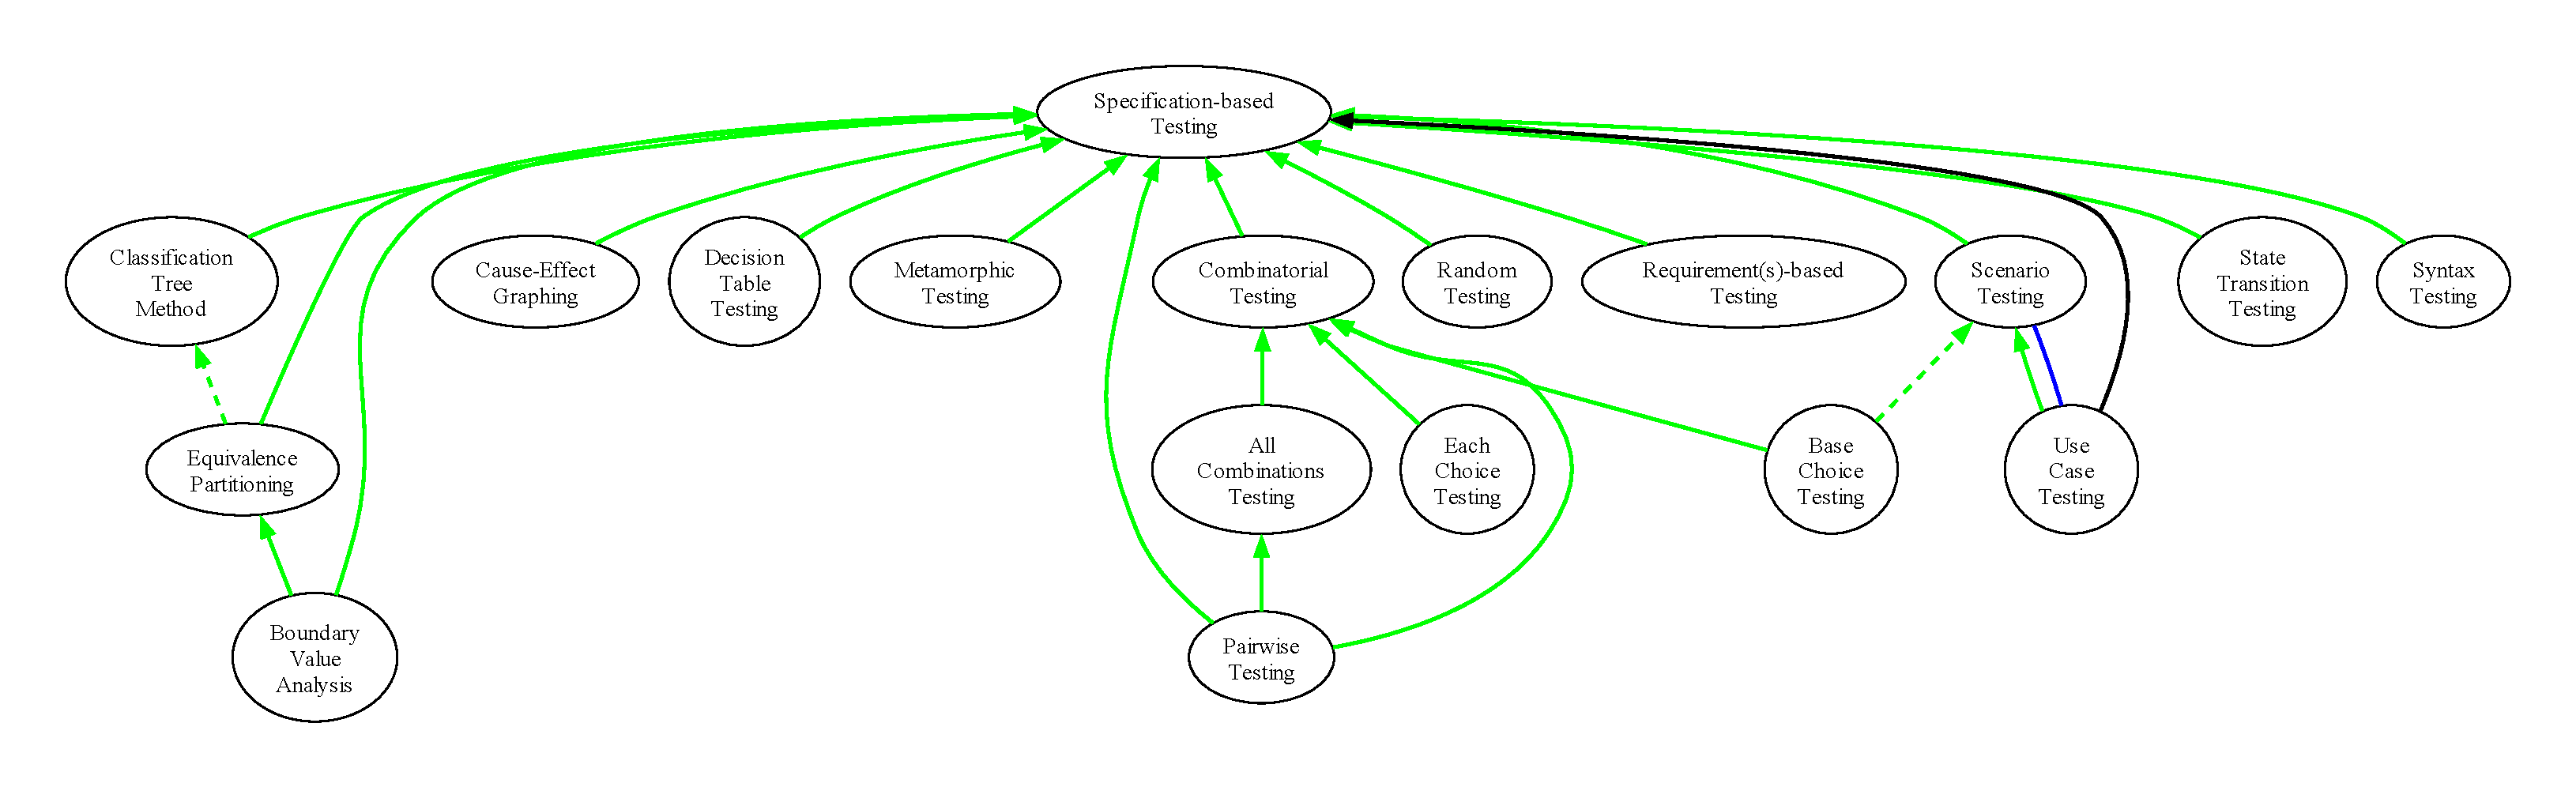
\includegraphics[width=\linewidth]{assets/graphs/specBasedGraph.pdf}
            \caption{``Superset'' relations.}
            \label{fig:specBasedGraph}
        \end{subfigure}
        \begin{subfigure}[t]{.45\linewidth}
            \centering
            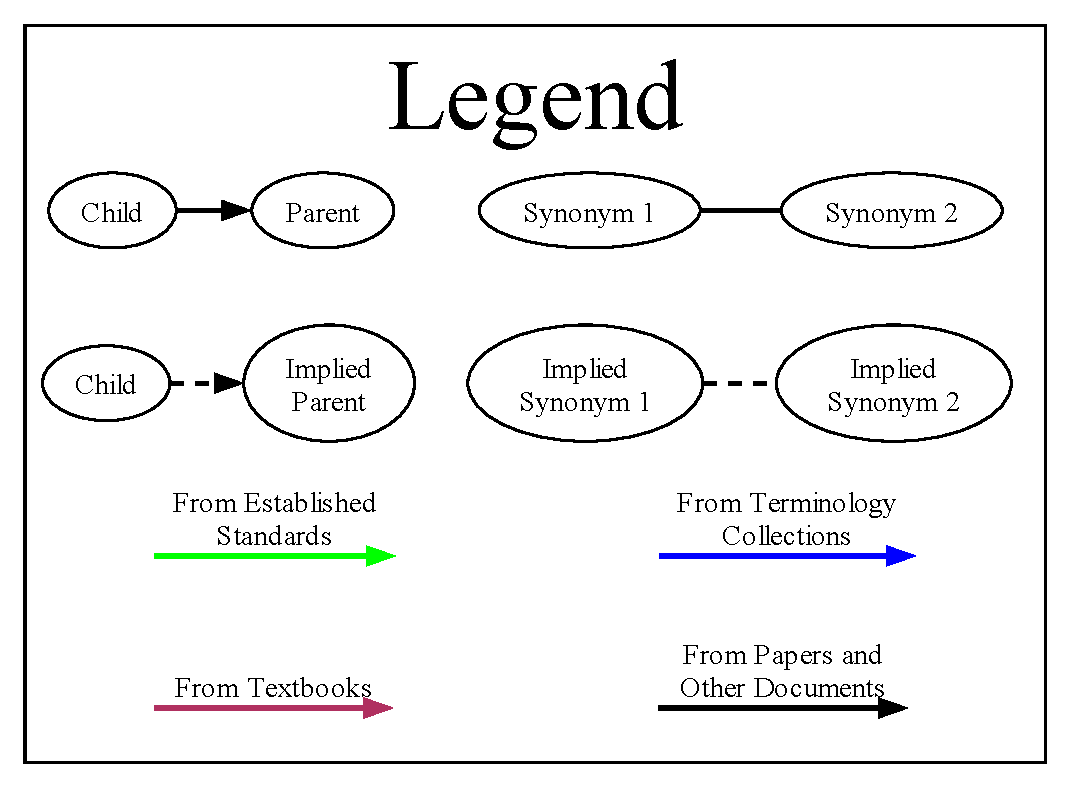
\includegraphics[width=\linewidth]{assets/graphs/parChdLegend.pdf}
        \end{subfigure}
        \begin{subfigure}[t]{.5\linewidth}
            \centering
            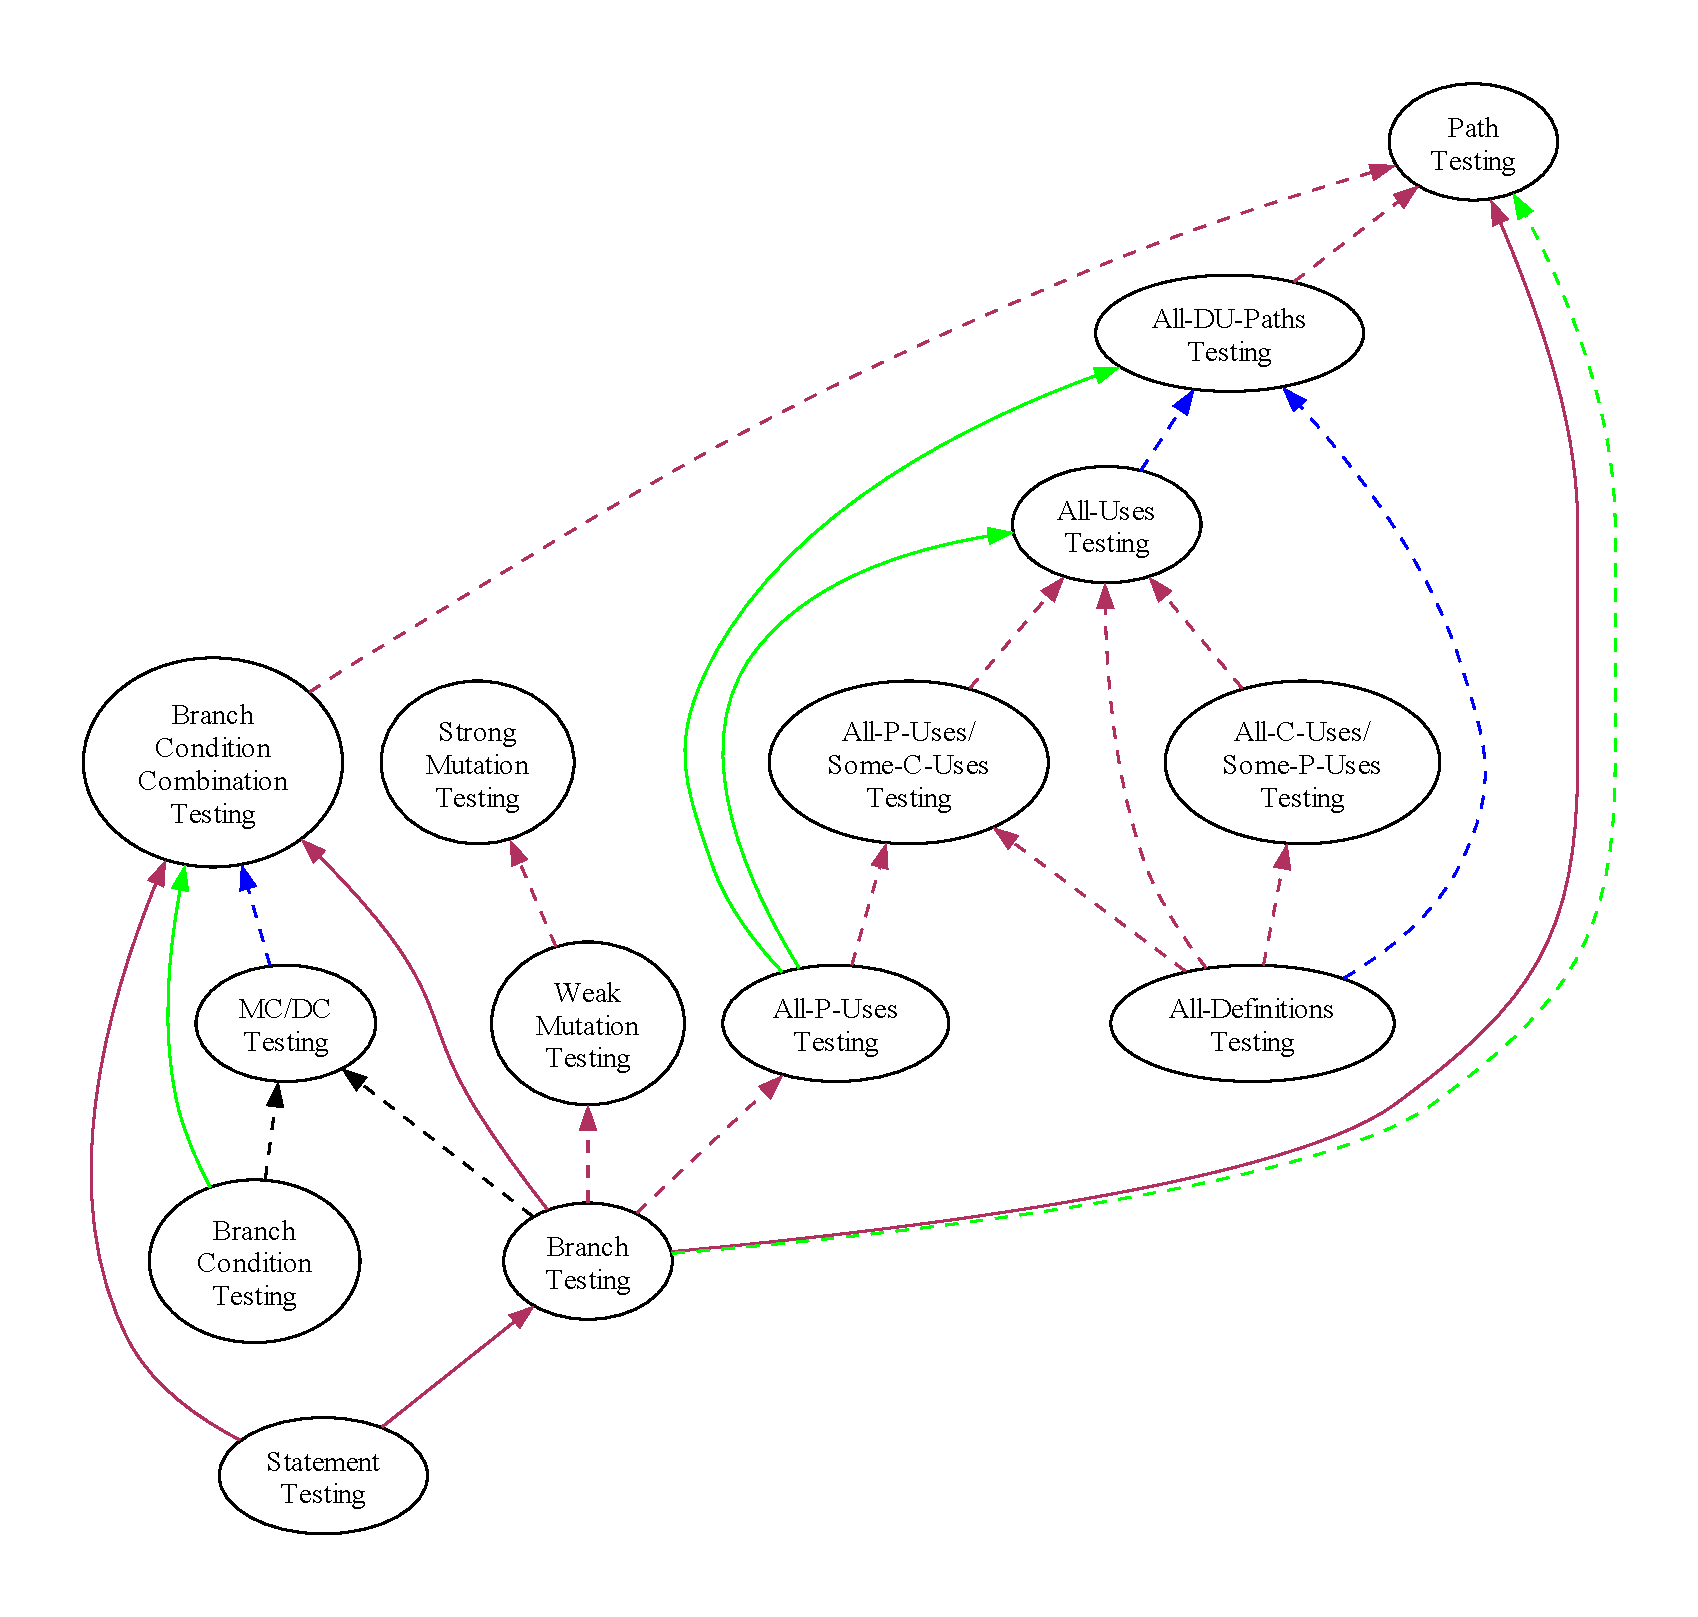
\includegraphics[width=\linewidth]{assets/graphs/subsumesGraph.pdf}
            \caption{``Subsume'' relations.}
            \label{fig:subsumesGraph}
        \end{subfigure}
        \caption{Graphs of different classes of parent-child relations.}
        \label{fig:parChdGraphs}
    \end{figure}
}

\newcommand{\ExampleGraph}{
    \begin{figure*}
        \begin{subfigure}[b]{0.275\linewidth}
            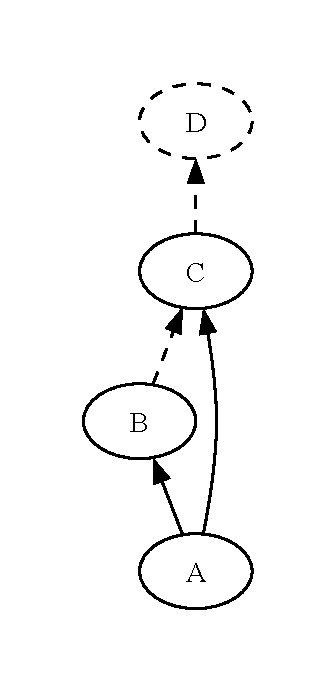
\includegraphics[width=\linewidth]{assets/graphs/ExampleGlossaryGraph.pdf}
            \caption{Graph from \\ \Cref{tab:exampleGlossary}.}
            \label{fig:exampleGraph}
        \end{subfigure}
        \centering
        \begin{subfigure}[b]{0.7\linewidth}
            \centering
            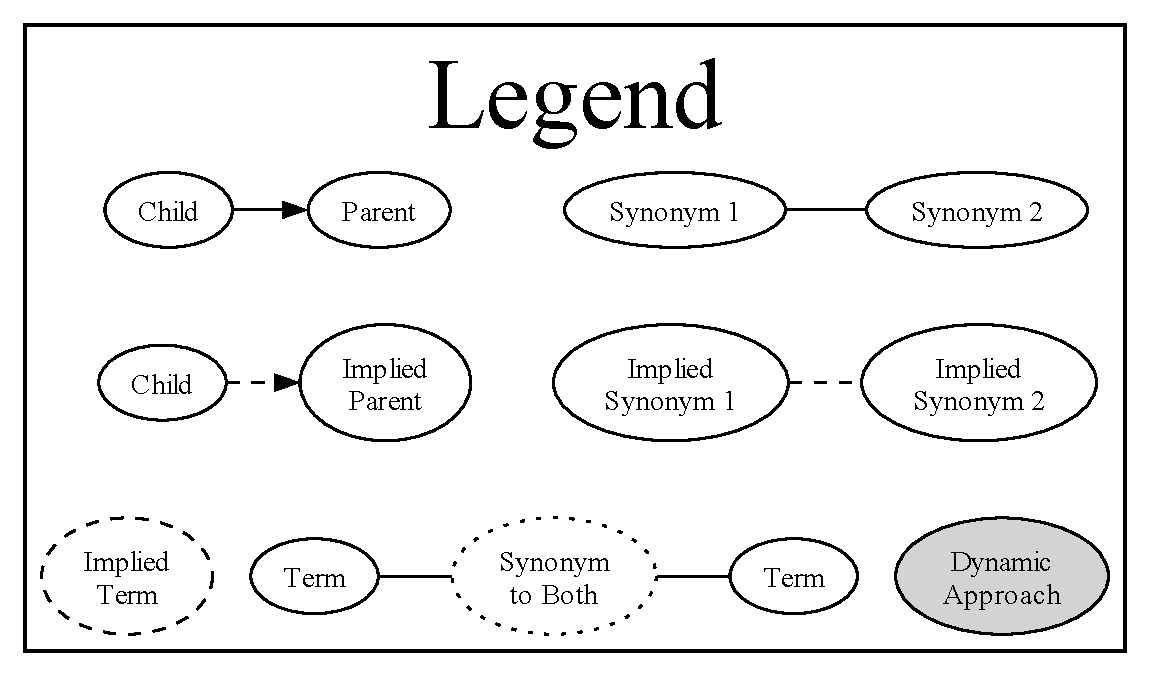
\includegraphics[width=\linewidth]{assets/graphs/manual/manualLegend.pdf}
            \hspace{5cm}\begin{subfigure}[t]{0.475\linewidth}
                \includegraphics[width=1.1\linewidth]{assets/graphs/rigidExampleGlossaryGraph.pdf}
                \caption{Rigid graph from\\\Cref{tab:exampleGlossary}.}
                \label{fig:rigidExampleGraph}
            \end{subfigure}
            \begin{subfigure}[t]{0.475\linewidth}
                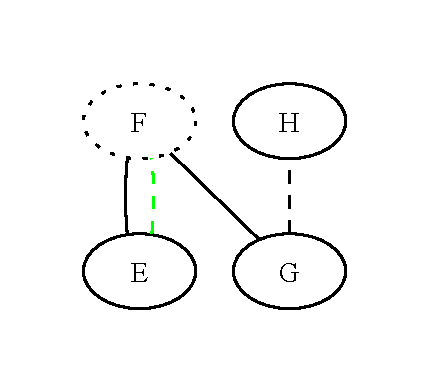
\includegraphics[width=1.1\linewidth]{assets/graphs/SynExampleGlossaryGraph.pdf}
                \caption{Graph from \Cref{tab:synExampleGlossary}.}
                \label{fig:synExampleGraph}
            \end{subfigure}
        \end{subfigure}
        \begin{subfigure}[t]{0.25\linewidth}
            \centering
            \includegraphics[width=1.2\linewidth]{assets/graphs/SelfExampleGlossaryGraph.pdf}
            \caption{Self-loop graph.}
            \label{fig:selfExampleGraph}
        \end{subfigure}
        \hfill
        \begin{subfigure}[t]{0.425\linewidth}
            \centering
            \includegraphics[width=0.6\linewidth]{assets/graphs/ParSynExampleGlossaryGraph.pdf}
            \caption{Graph of a pair of terms with a \hyperref[par-chd-rels]{parent-child} \emph{and} synonym relation.}
            \label{fig:parSynExampleGraph}
        \end{subfigure}
        \hfill
        \begin{subfigure}[t]{0.25\linewidth}
            \centering
            \includegraphics[width=1.4\linewidth]{assets/graphs/StaticExampleGlossaryGraph.pdf}
            \caption{Static graph.}
            \label{fig:staticExampleGraph}
        \end{subfigure}
        \caption{Example generated graphs.}
        \label{fig:exampleGraphs}
    \end{figure*}
}

\newcommand{\recoveryGraphs}{
    % Only top or bottom to comply with IEEE guidelines
    \begin{figure}[bt!]
        \centering
        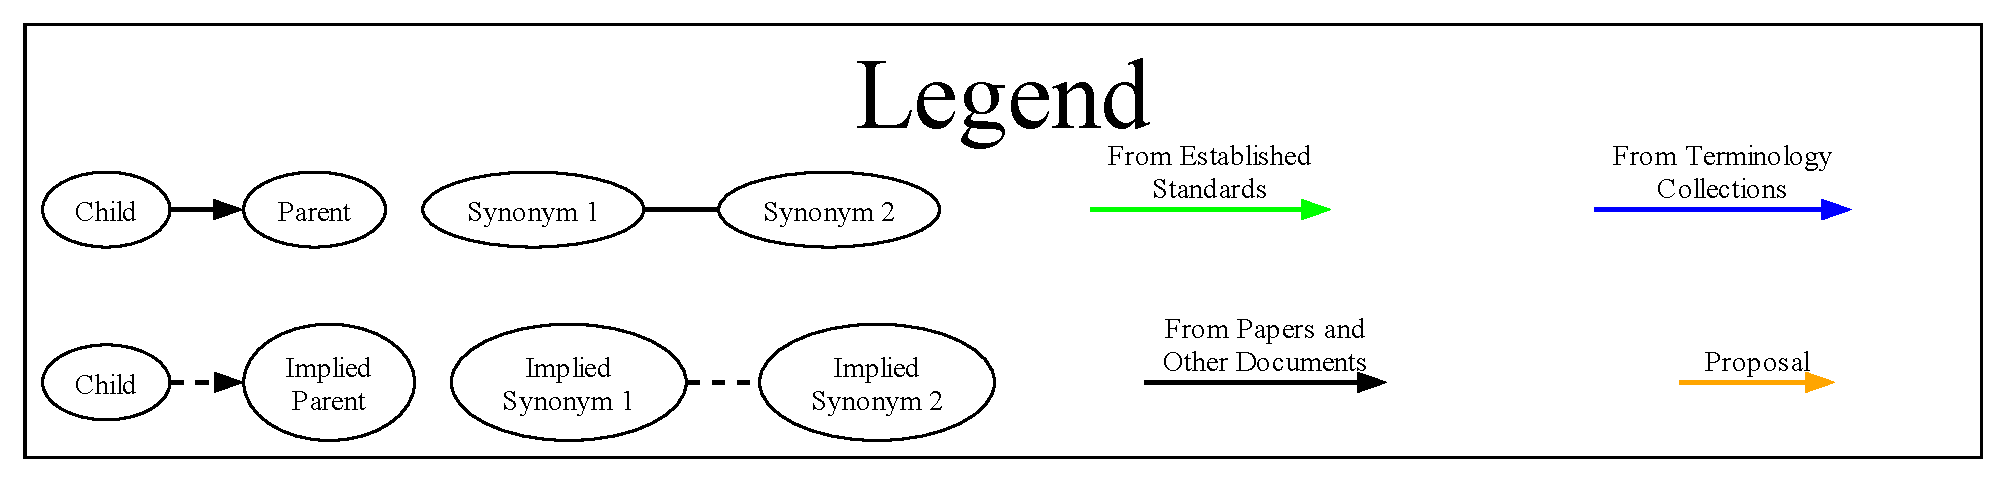
\includegraphics[width=\linewidth]{assets/graphs/recoveryLegend.pdf}
        \begin{subfigure}[b]{.475\linewidth}
            \centering
            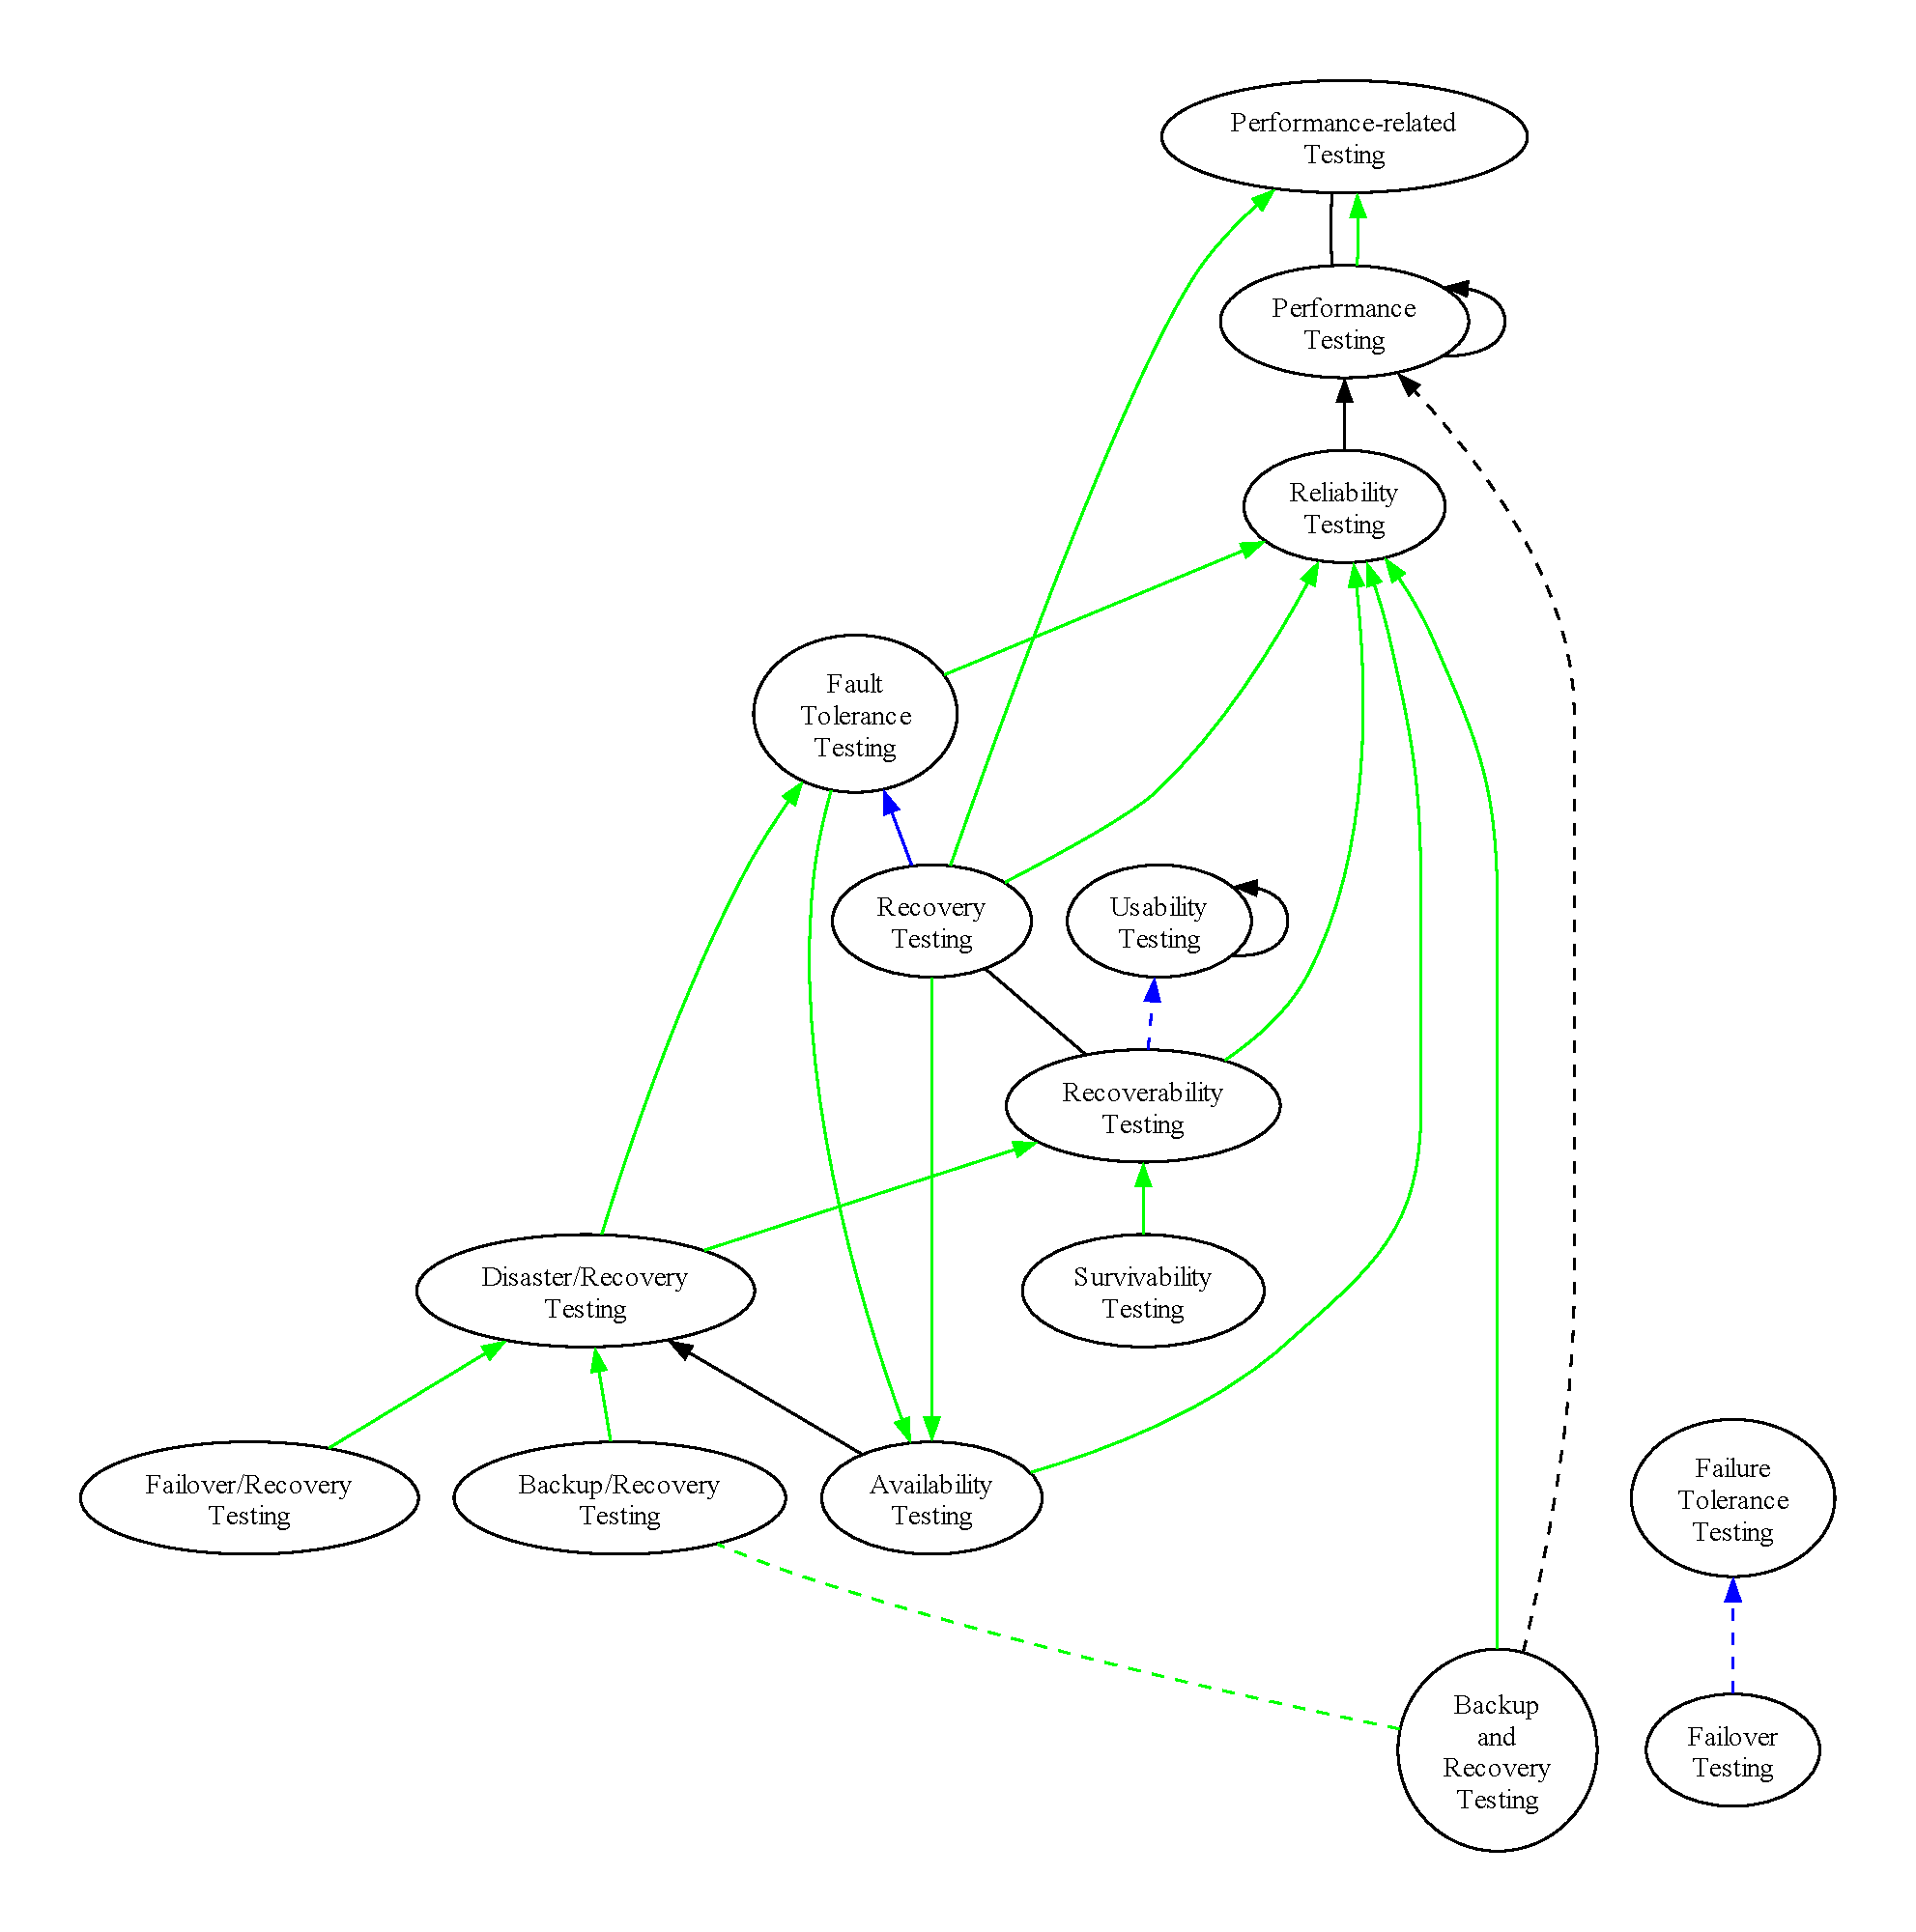
\includegraphics[width=\linewidth]{assets/graphs/recoveryGraph.pdf}
            \caption{Graph of current relations.}
            \label{fig:rec-graph-current}
        \end{subfigure}
        \begin{subfigure}[b]{.475\linewidth}
            \centering
            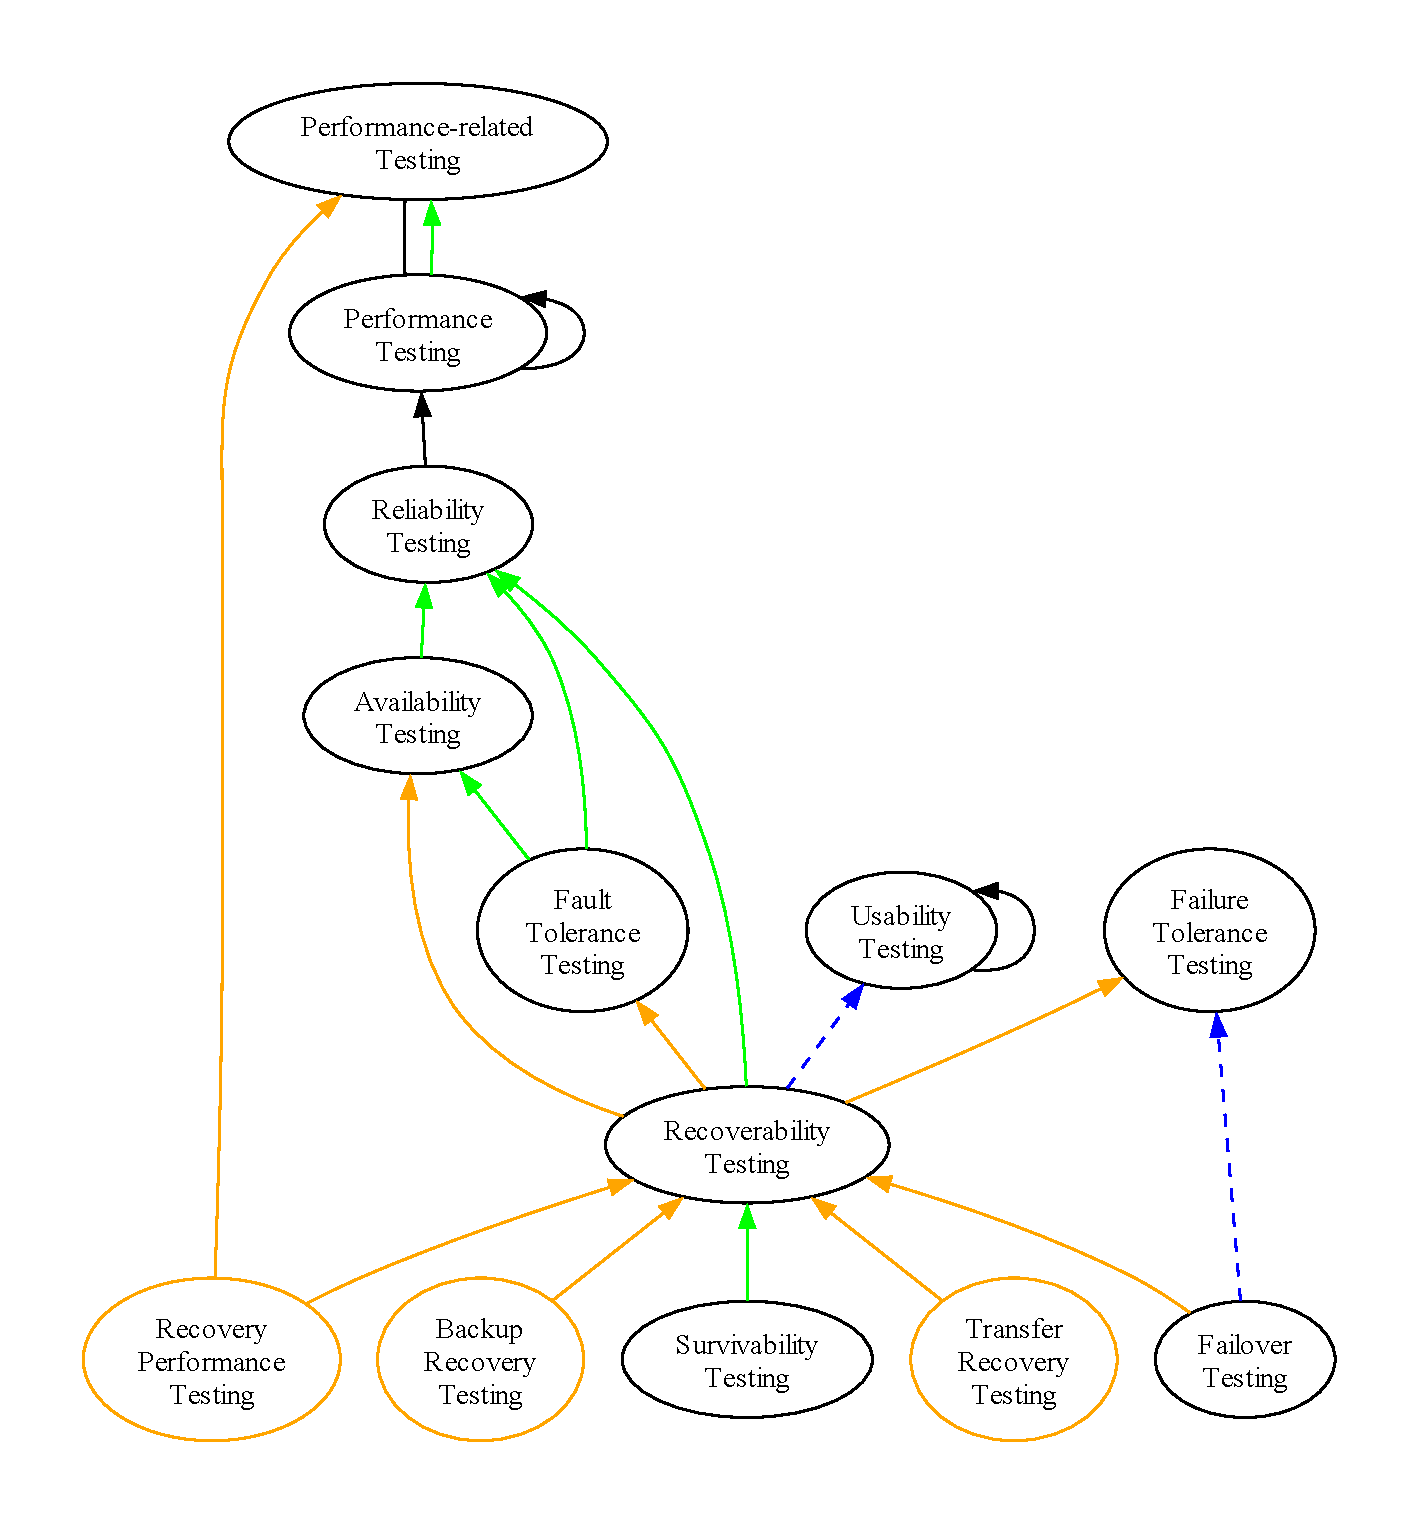
\includegraphics[width=\linewidth]{assets/graphs/recoveryProposedGraph.pdf}
            \caption{Graph of proposed relations.}
            \label{fig:rec-graph-proposed}
        \end{subfigure}
        \caption{Graphs of relations between terms related to recovery testing.}
        \label{fig:recoveryGraphs}
    \end{figure}
}

\newcommand{\scalGraphs}{
    % Only top or bottom to comply with IEEE guidelines
    \begin{figure}[b!]
        \centering
        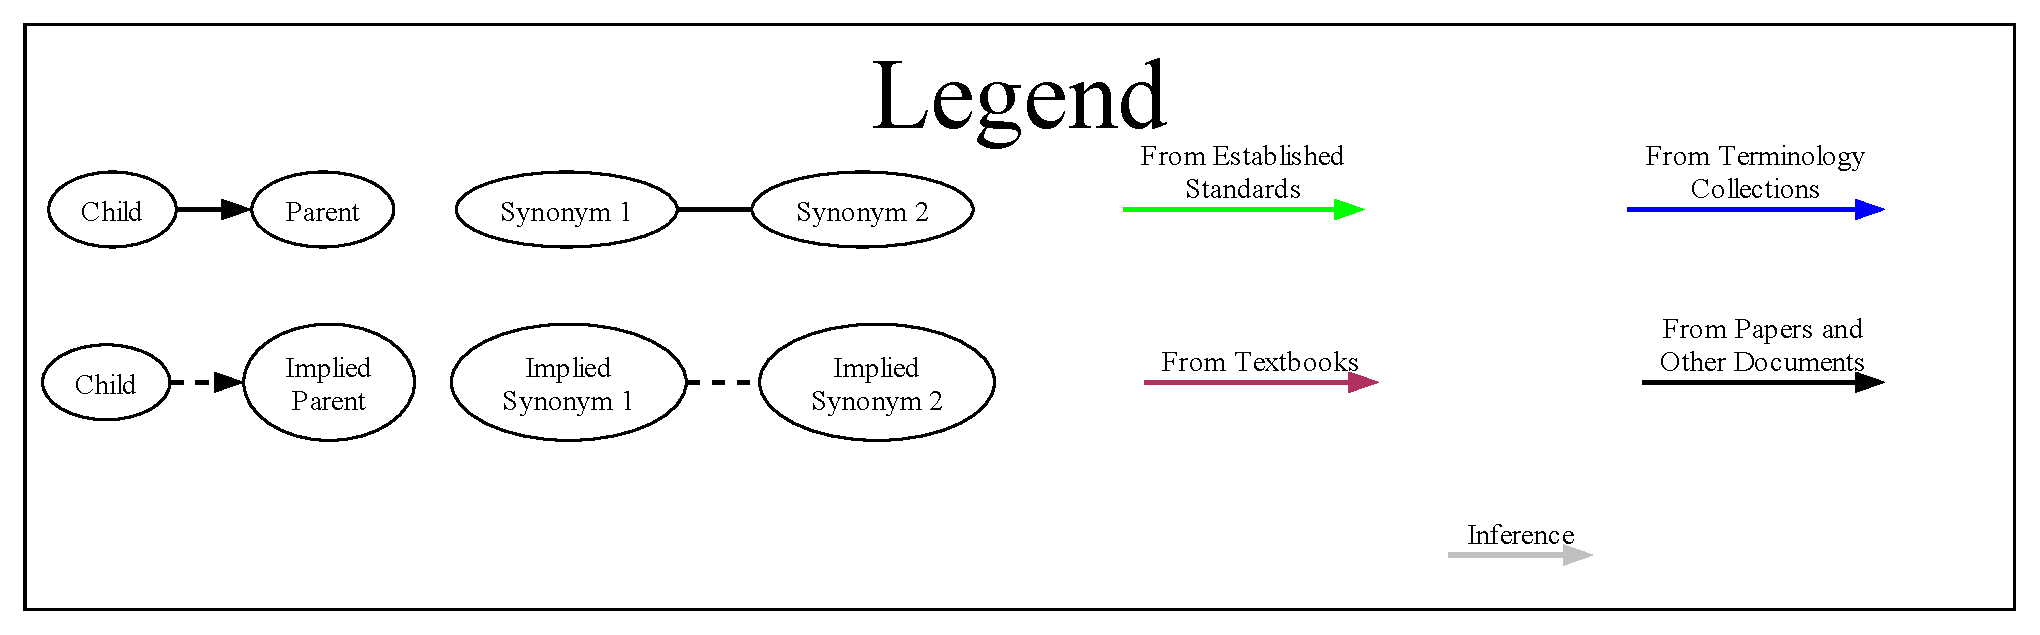
\includegraphics[width=\linewidth]{assets/graphs/scalabilityLegend.pdf}
        \begin{subfigure}[b]{.475\linewidth}
            \centering
            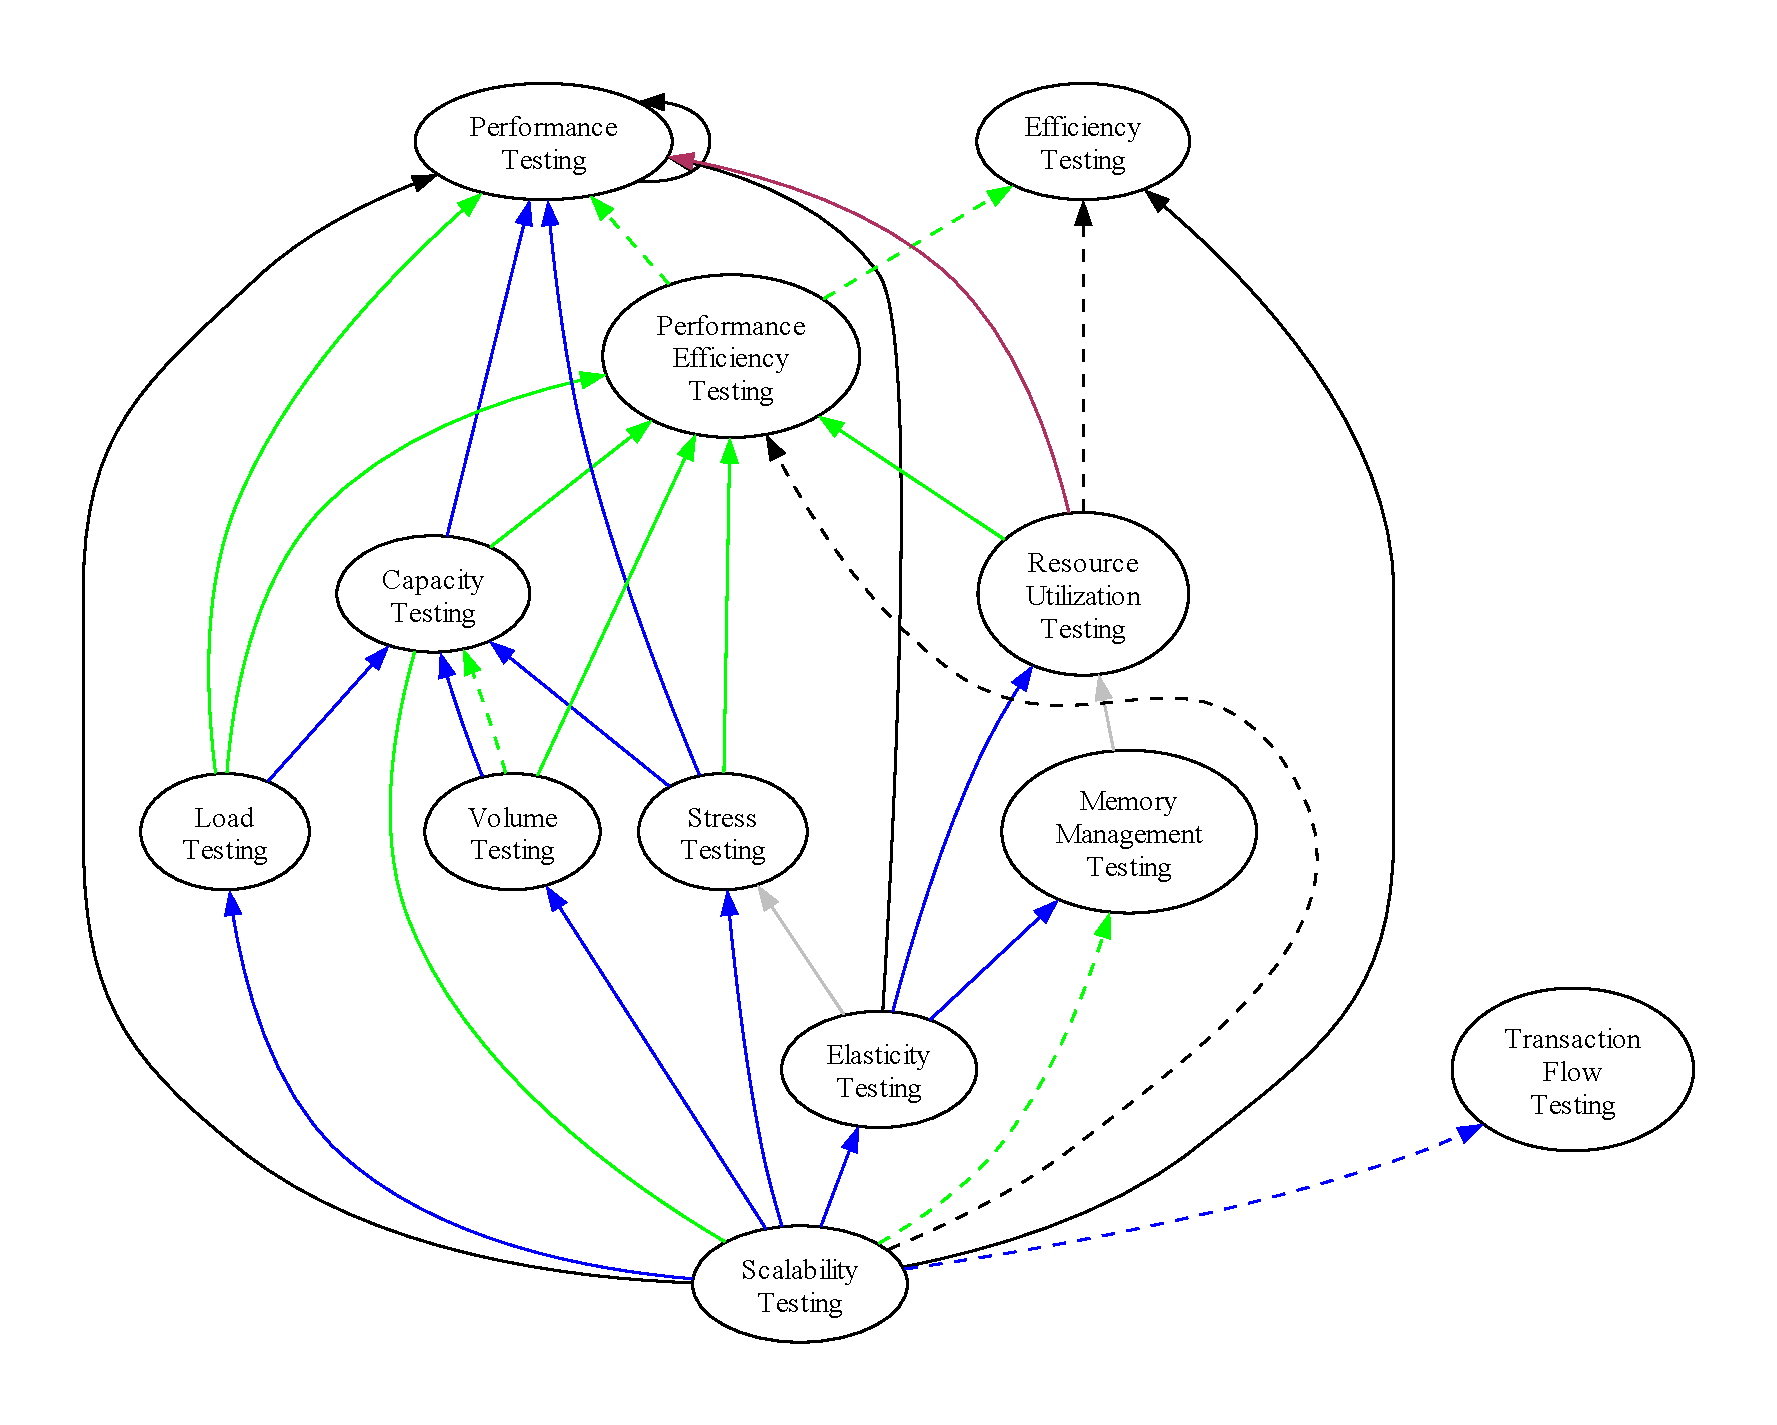
\includegraphics[width=\linewidth]{assets/graphs/scalabilityGraph.pdf}
            \caption{Graph of current relations.}
            \label{fig:scal-graph-current}
        \end{subfigure}
        \begin{subfigure}[b]{.475\linewidth}
            \centering
            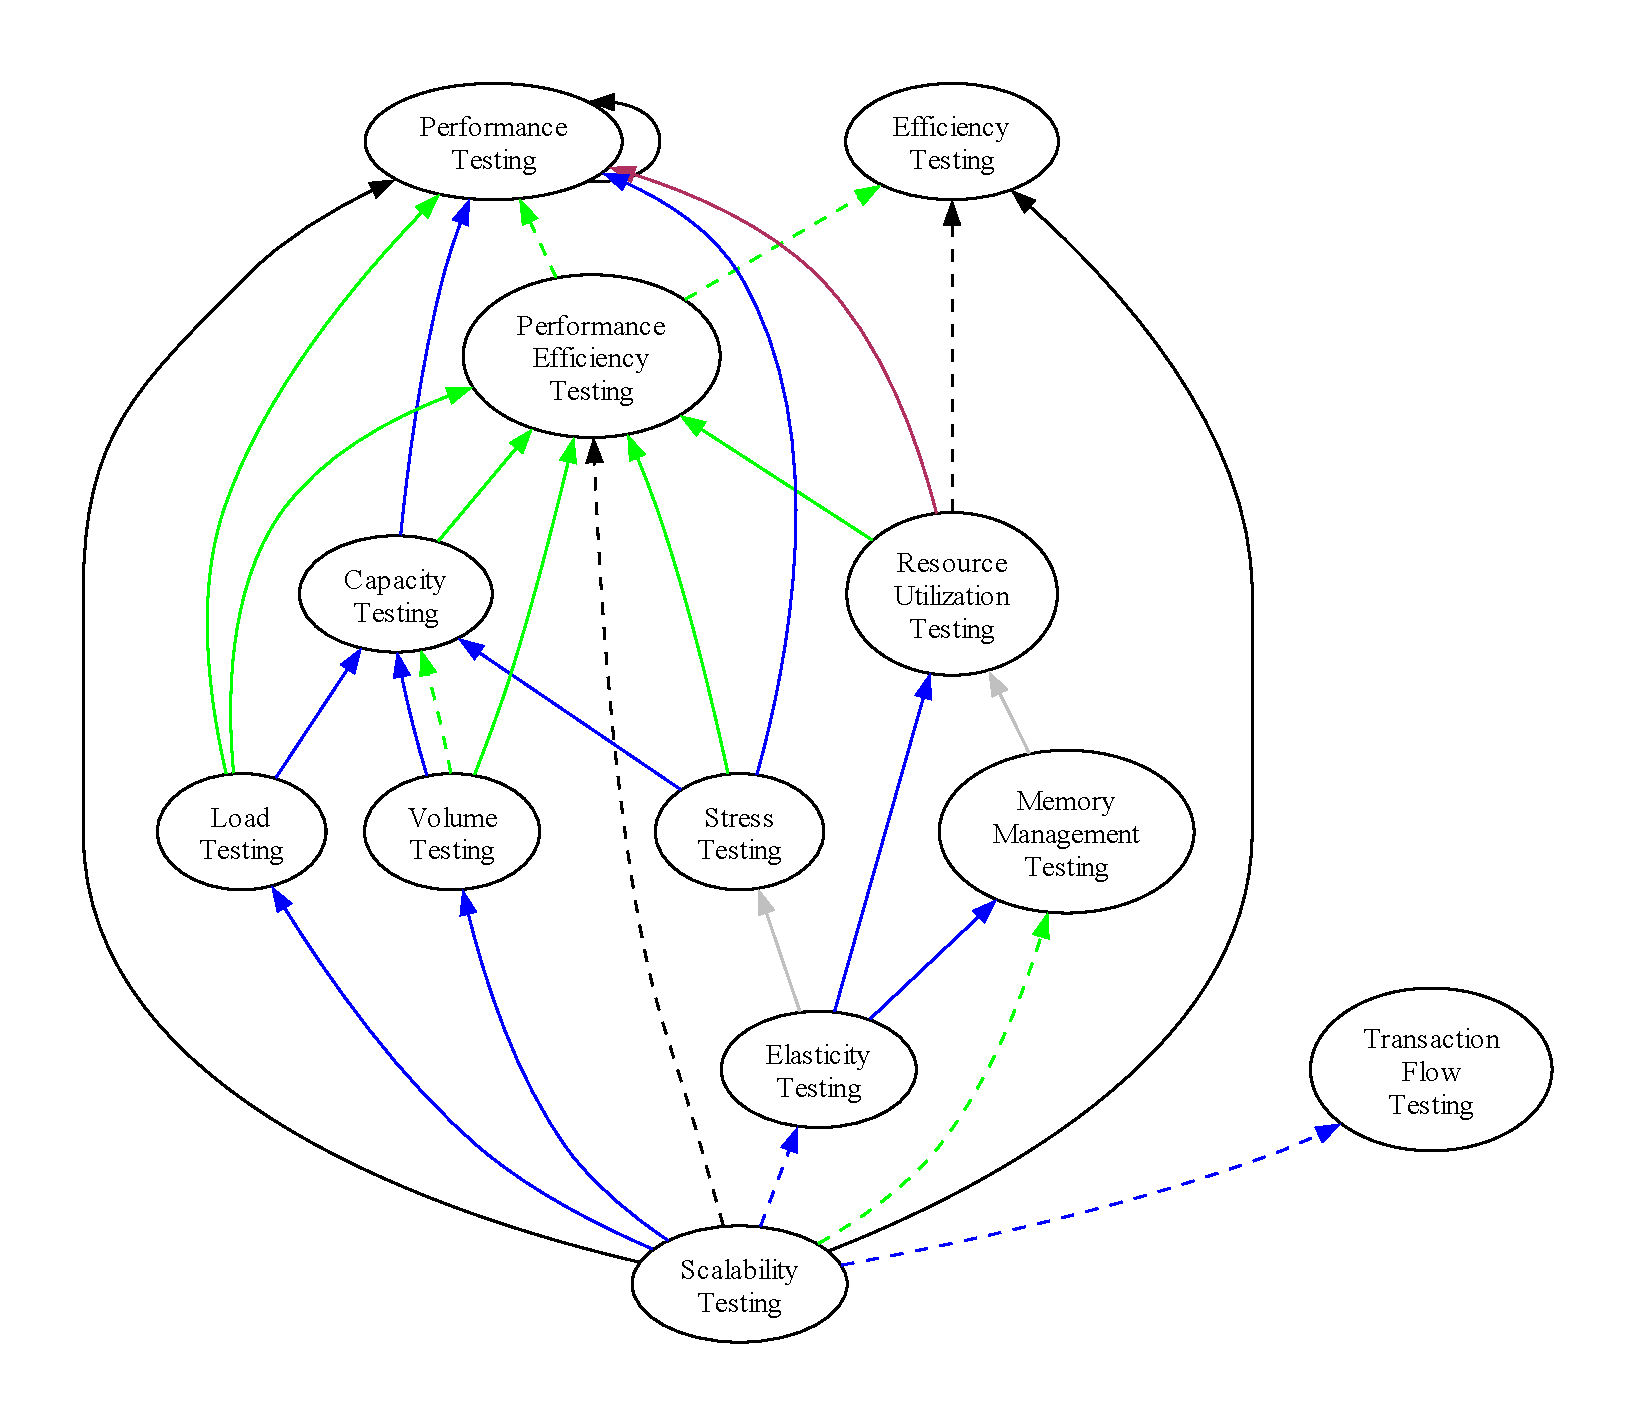
\includegraphics[width=\linewidth]{assets/graphs/scalabilityProposedGraph.pdf}
            \caption{Graph of proposed \ifnotpaper \else \\ \fi relations.}
            \label{fig:scal-graph-proposed}
        \end{subfigure}
        \caption{Graphs of relations between terms related to scalability testing.}
        \label{fig:scalGraphs}
    \end{figure}
}

\newcommand{\performanceGraph}{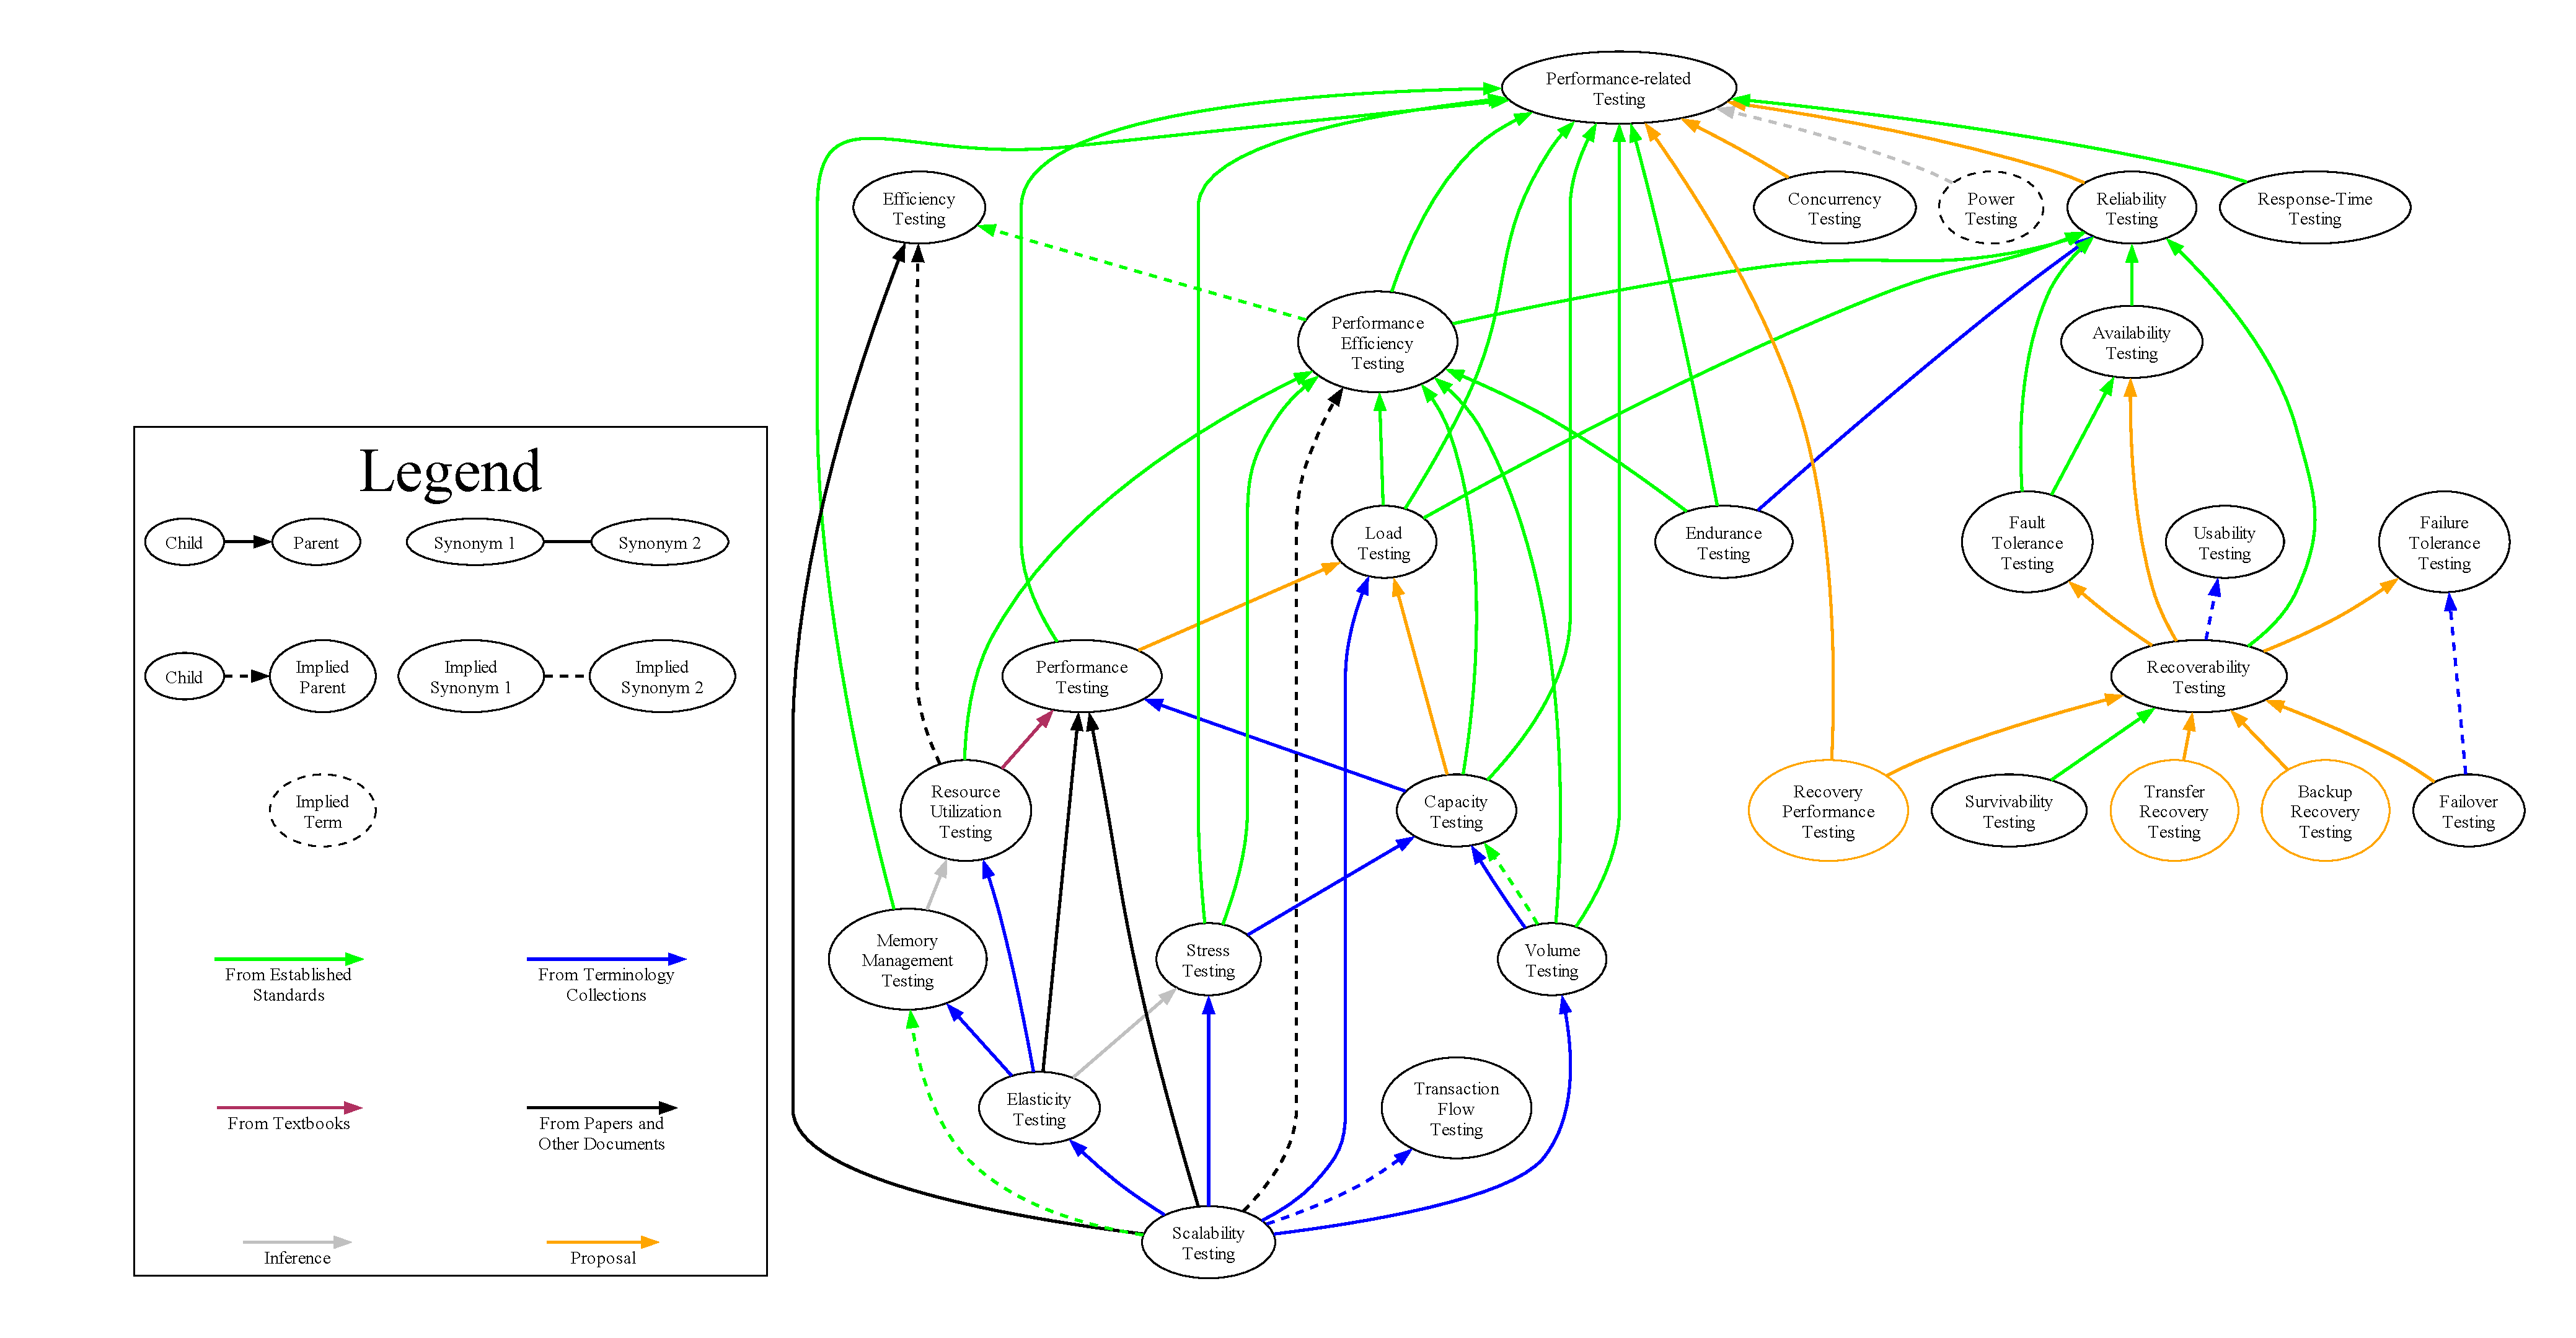
\includegraphics[width=\linewidth]{assets/graphs/performanceProposedGraph.pdf}}

%------------------------------------------------------------------------------
% Images & Figures
%------------------------------------------------------------------------------

\newcommand{\drasilLogo}{assets/images/drasil_logo.png}
\newcommand{\drasilLogoImg}{\input{assets/images/drasil_logo}}
\newcommand{\refDrasilLogoImg}{\Cref{fig:drasilLogo}}

%------------------------------------------------------------------------------
% Tables
%------------------------------------------------------------------------------

% Organization of files
\newcommand{\organizationTable}{\input{assets/tables/organization}}

\newcommand{\ieeeCatsTable}{\input{assets/tables/ieeeCats}}
\newcommand{\otherCatsTable}{\input{assets/tables/otherCats}}
\newcommand{\otherCategorizationsTable}{\input{assets/tables/otherCategorizations}}

\newcommand{\flawMnfstsTable}{\input{assets/tables/flawMnfsts}}
\newcommand{\flawDmnsTable}{\input{assets/tables/flawDmns}}

\newcommand{\testReqsTable}{\input{assets/tables/testReqs}}



% Enable links within the document
\usepackage{hyperref}
\hypersetup{
    linkcolor=red,
    urlcolor=red,
    breaklinks=true,
    pdftitle={\thesisTitle{}},
}
\urlstyle{rm} % Make URL styled fonts match hyperref's hrefs
\usepackage[capitalize]{cleveref} % Fixes capitalization of internal references

% General Utility Functions
\def\sWidth{3.4cm}
\def\tWidth{0.7cm}
\newif\ifnotpaper

%------------------------------------------------------------------------------
% Reused in seminar slides
%------------------------------------------------------------------------------

\def\rqatext{What testing approaches do the literature describe?}
\def\rqbtext{Are these descriptions consistent?}
\def\rqctext{Can we systematically resolve any of these inconsistencies?}

\def\addTextEx{For example, \citetISTQB{} \multiAuthHelper{cite}
    \citet{GerrardAndThompson2002} as the original source
    for \ifnotpaper their \else its \fi definition of ``scalability'' (see
    \Cref{scal-test-rec}) which we verify by looking at this original source.}

\def\supers{Dr.~Spencer Smith and Dr.~Jacques Carette}
\def\supersAck{\supers{} have been great supervisors and valuable sources of
    guidance and feedback}

%------------------------------------------------------------------------------
% Spacing Options
%------------------------------------------------------------------------------

\newcommand{\thesisForceSingleSpacing}{\singlespacing}
\newcommand{\thesisForceDoubleSpacing}{\doublespacing}

%------------------------------------------------------------------------------
% Portable HREFs
%------------------------------------------------------------------------------

% Common variant
\newcommand{\porthref}[2]{\href{#2}{#1}\printOnlyFootnote{\url{#2}}}

% Custom URLs
\newcommand{\porthreft}[3]{\href{#3}{#1}\printOnlyFootnote{\href{#3}{#2}}}
% Inside of some environments, footnote marks aren't registered properly, so we
% need to manually write the "text" part
\newcommand{\porthreftm}[2]{\href{#2}{#1\printOnlyFootnoteMark}}

\newcommand{\formatPaper}[2]{%
    \ifnotpaper #1{#2}%
    \else \underline{#2}%
    \fi
}

\def\refHelper{\ifnotpaper\else Reference \fi}
\newcommand\multiAuthHelper[1]{\ifnotpaper #1\else #1s\fi}
\def\docType{\ifnotpaper thesis%
    \else paper%
    \fi}

\newcommand\flawref[1]{%
    \ifnotpaper \labelcref{#1}%
    \else \Cref{#1}%
    \fi}

\newcommand\ifblind[2]{\IfEndWith*{\jobname}{_blind}{#1}{#2}}

%------------------------------------------------------------------------------
% Generic "chunks" that get reused
%------------------------------------------------------------------------------

\def\oneSrcDistinct{we make a distinction between ``self-contained'' flaws and
    ``internal'' flaws\thesisissueref{137,138}.}

\def\highLvlScope{a high-level overview of what is in scope\ifnotpaper; see
    \Cref{app-scope} for more detailed discussion on what we include and
    exclude\fi}

\def\listAllSrcs{\ifnotpaper\ and list all sources in each tier
        in \Cref{app-src-tiers}\fi}

\newcommand\defRel[3]{We can formally define the #1 relation $#2$ on the set
    $T$ of terms used by the literature to describe test approaches based on #3.}

\NewDocumentCommand{\approachFields}{s}{%
    definitions, categories\IfBooleanTF{#1}{}{\ (see \Cref{cats-def})},
    synonyms\IfBooleanTF{#1}{}{\ (see \Cref{syn-rels})}, and
    parents\IfBooleanTF{#1}{}{\ (see \Cref{par-chd-rels})}%
}

\def\displayNL{\\
    $\,\hookrightarrow\,$\quad }

\DeclareDocumentCommand\seeSrcCode{ m m m g }{%
    (see the \href{
        https://github.com/samm82/TestingTesting/blob/#1/#2\#L#3%
        \IfNoValueF{#4}{-L#4}}
    {relevant source code})%
}

\def\ourApproachGlossary{\ifblind{our test approach glossary}{\href{
            https://github.com/samm82/TestingTesting/blob/main/ApproachGlossary.csv
        }{our test approach glossary}}}

\def\accelTolTest{astronauts \citep[p.~11]{MorgunEtAl1999}, aviators
    \citep[pp.~27, 42]{HoweAndJohnson1995}, or catalysts
    \citep[p.~1463]{LiuEtAl2023}}
\NewDocumentCommand{\orthTestIntro}{s}{%
    \IfBooleanTF{#1}{s}{S}ome test approaches appear to be combinations of
    other (seemingly orthogonal) approaches}
\def\impKeywords{``implied'', ``can be'', ``sometimes'', ``should be'',
    ``ideally'', ``usually'', ``most'', ``likely'', ``often'', ``if'', and
    ``although''\utd{}}

\def\recFigs{\Cref{fig:recoveryGraphs,fig:perf-graph}} % fig:scalGraphs

% Define common footnotes about IEEE testing terms for reuse
\newcommand{\distinctIEEE}[1]{distinct from the notion of ``test #1'' described
    in \Cref{tab:ieeeCats}.}
\newcommand{\notDefDistinctIEEE}[1]{\footnote{Not formally defined, but
        \distinctIEEE{#1}}}
% % Defined with help from GitHub Copilot
% \NewDocumentCommand{\gerrardDistinctIEEE}{s m}{%
%     \IfBooleanTF{#1}{}{\footnote}%
%     {``Each type of test addresses a different risk area''
%         \citep[p.~12]{Gerrard2000a}, which is \distinctIEEE{#2}}%
% }

\NewDocumentCommand{\multiCatIntro}{s}{%
    \IfBooleanTF{#1}{T}{we automatically detect t}est approaches with more
    than one category that violate our assumption of orthogonality
    (see \Cref{orth-approach})}

\NewDocumentCommand{\parSynFlaw}{s}{%
    \IfBooleanTF#1{P}{p}airs of synonyms where one is a subapproach of the
    other; these relations cannot coexist since synonym relations are symmetric
    while parent-child relations are asymmetric (as outlined in
    \Cref{syn-rels,par-chd-rels}, respectively).}
\NewDocumentCommand\parSynIntro{s}{%
    \IfBooleanTF#1{t}{T}here are also \parSynFlaw{}
    \IfBooleanTF#1{Below are all}{We identify} \parSynCount{}
    of these pairs\IfBooleanTF#1{\ that we identify}{} through automatic
    analysis of our generated visualizations\ifnotpaper\ as described in
        \Cref{auto-flaw-detect}\fi}

% Examples of flaws
\def\bugPattonFlaw{\citet[pp.~13\==14]{Patton2006} ``just call[s] it what it
    is and get[s] on with it'', abandoning these four terms, ``problem'',
    ``incident'', ``anomaly'', ``variance'', ``inconsistency'', ``feature'' (!),
    and ``a list of unmentionable terms'' in favour of ``bug''; after all,
    ``there's no reason to dice words''!}
\NewDocumentCommand\tourFlaw{s}{%
    \IfBooleanTF#1{t}{T}he structure of tours can be defined as either quite
    general \citep[p.~34]{IEEE2022} or ``organized around a special focus''
    \citepISTQB{}\IfBooleanTF#1{}{.}}
\def\alphaFlaw{Alpha testing is performed by ``users within the organization
    developing the software'' \citep[p.~17]{IEEE2017}, ``a small, selected
    group of potential users'' \citep[p.~5\=/8]{SWEBOK2025}, or ``roles outside
    the development organization'' conducted ``in the developer's test
    environment'' \citepISTQB{}.}
\def\loadFlaw{Load testing is performed with loads ``between anticipated
    conditions of low, typical, and peak usage'' \citep[p.~5]{IEEE2022} or
    loads that are as large as possible \citep[p.~86]{Patton2006}.}
\NewDocumentCommand{\seeRefMissing}{s}{%
    \IfBooleanTF#1{}{\refHelper} \citet[p.~42]{Kam2008} says ``See
    \emph{boundary value analysis},'' for the glossary entry of ``boundary
    value testing'' but does not include ``boundary value analysis'' in the
    glossary.}
\def\qualImprovFlaw{\citet[p.~5\=/4]{SWEBOK2025} says that quality improvement,
    along with quality assurance, is an aspect of testing that involves
    ``defining methods, tools, skills, and practices to achieve the specific
    quality level and objectives''; while testing that a system possesses
    certain qualities is in scope, actively improving the system in response is
    \emph{not} part of testing.}
\NewDocumentCommand{\tolTestFlaw}{s}{%
    \IfBooleanTF#1{t}{T}he terms ``acceleration tolerance testing'' and
    ``acoustic tolerance testing'' do not seem to refer to software testing,
    but \citet[p.~56]{Firesmith2015} includes them regardless. Elsewhere,
    they seem to refer to testing the acoustic tolerance of rats
    \citep{HolleyEtAl1996} or the acceleration tolerance of \accelTolTest{},
    which which are not relevant to software testing.}
\def\errorGuessFlaw{Since the differences between the terms ``error'',
    ``failure'', ``fault'', and ``defect'' are significant and meaningful
    \ifnotpaper (\citealp[pp.~124, 165\todo{OG 2009}, 178\==179]{IEEE2017};
        \citeyear[pp.~96, 128, 139\==140]{IEEE2010};
        \citealp[pp.~5\=/3, 12\=/3]{SWEBOK2025}\footnote{
            \citet[p.~12\=/3]{SWEBOK2025} references the definitions given in
            \citep[pp.~124, 165, 178\==179]{IEEE2017}; while we would usually
            omit the former in favour of the original source, we include it
            here as an example of a flaw within a document.};
        \citealp[pp.~399\==400]{vanVliet2000})\else TODO: make macro\fi,
    error guessing should either be called:
    \begin{itemize}
        \item ``defect guessing'' if it is based on a ``checklist of potential
              defects'' \citep[p.~29]{IEEE2021c},
        \item ``failure guessing'' if it is based on ``the tester's knowledge
              of past failures'' \citeyearpar[p.~165]{IEEE2017}, or
        \item ``fault guessing'' if it is a ``fault-based technique''
              \citep[p.~4\=/9]{SWEBOK2014} that ``anticipate[s] the most
              plausible faults in each \acs{sut}'' \citep[p.~5\=/13]{SWEBOK2025}.
    \end{itemize}
    One (or multiple) of these proposed terms may be useful in tandem with
    ``error guessing'', which would focus on errors as traditionally defined
    and be a subapproach of error-based testing (implied by
    \citealp[p.~399]{vanVliet2000}).}
\NewDocumentCommand{\perfSecParFlaw}{s}{%
    \IfBooleanTF#1{p}{P}erformance testing and security testing are given as subtypes of
    reliability testing by \citet{ISO_IEC2023a}, but these are all listed
    separately by \citet[p.~53]{Firesmith2015}.}
\def\parSheetTestFlaw{``Par sheet testing'' from \citepISTQB{} seems to refer
    to \ifnotpaper the specific example mentioned in \flawref{specific-istqb}
    \else some specific example it does not cite \fi and does not seem more
    widely applicable, since a ``PAR sheet'' is ``a list of all the symbols on
    each reel of a slot machine'' \citep{Bluejay2024}.}
\NewDocumentCommand{\redBoxFlaw}{s}{%
    \IfBooleanTF#1{t}{T}he incorrect claim that ``white-box
    testing'', ``grey-box testing'', and ``black-box testing'' are
    synonyms for ``module testing'', ``integration testing'', and
    ``system testing'', respectively, \ifnotpaper (see
        \flawref{dubious-syns}) \fi casts doubt on the claim that
    ``red-box testing'' is a synonym for ``acceptance testing''
    \citep[p.~18]{SneedAndGöschl2000}\todo{OG Hetzel88}\ifnotpaper\
        (see \flawref{dubious-red-box-syn})\fi.}

\NewDocumentCommand{\defLabelDistinct}{s}{%
    \IfBooleanTF#1{t}{T}erms can be thought of as definition-label pairs,
    but there is a meaningful distinction between definition flaws and label
    flaws}

% Used in parSyns tables
\def\ftrnote{Fault tolerance testing may also be a subapproach of
    reliability testing \ifnotpaper
        \citetext{\citealp[p.~375]{IEEE2017}; \citealp[p.~7\=/10]{SWEBOK2025}}%
    \else \cite[p.~375]{IEEE2017}, \cite[p.~7\=/10]{SWEBOK2025}%
    \fi, which is distinct from robustness testing \citep[p.~53]{Firesmith2015}.}
\def\specfn{%
    % Flaw count (MISS, SYNS): ISTQB | {IEEE2017}
    \refHelper \citetISTQB{} \multiAuthHelper{cite} \citet[p.~431]{IEEE2017}
    for \ifnotpaper their \else its \fi definition of ``functional testing''
    but \multiAuthHelper{exclude} the transitive synonym relationship
    (see \Cref{syn-rels}) \ifnotpaper they give \else it gives \fi to
    ``specification-based testing''.
    % Flaw count (CONTRA, SYNS): {IEEE2017} implied by {IEEE2021c} {IEEE2017} | {IEEE2022} {IEEE2021c} ISTQB
    % Assertion: {Kam2008} {vanVliet2000}
    These terms are also defined separately elsewhere \ifnotpaper
        (\citeyear[Fig.~2]{IEEE2022}; \citeyear[pp.~8, 49, 125]{IEEE2021c})\else
        \cite{IEEE2022}, \cite{IEEE2021c}\fi, further supporting that they are
    not synonyms.
}
\def\ucstn{%
    % Flaw count (CONTRA, SYNS): ISTQB | {IEEE2022}
    \refHelper \citet[Fig.~2]{IEEE2022} also \multiAuthHelper{list}
    ``use case testing'' and ``scenario testing'' separately, further
    supporting that these terms are not synonyms.}

%------------------------------------------------------------------------------
% For populating values from files
%------------------------------------------------------------------------------

\ExplSyntaxOn
\ior_new:N \g_hringriin_file_stream

\NewDocumentCommand{\ReadFile}{mm}
{
    \hringriin_read_file:nn { #1 } { #2 }
    \cs_new:Npn #1 ##1
    {
        \str_if_eq:nnTF { ##1 } { * }
        { \seq_count:c { g_hringriin_file_ \cs_to_str:N #1 _seq } }
        { \seq_item:cn { g_hringriin_file_ \cs_to_str:N #1 _seq } { ##1 } }
    }
}

\cs_new_protected:Nn \hringriin_read_file:nn
{
    \ior_open:Nn \g_hringriin_file_stream { #2 }
    \seq_gclear_new:c { g_hringriin_file_ \cs_to_str:N #1 _seq }
    \ior_map_inline:Nn \g_hringriin_file_stream
    {
        \seq_gput_right:cx
        { g_hringriin_file_ \cs_to_str:N #1 _seq }
        { \tl_trim_spaces:n { ##1 } }
    }
    \ior_close:N \g_hringriin_file_stream
}

\ExplSyntaxOff

% Define/read values for Undefined Terms methodology for reuse and calculation!
\ReadFile{\undefTermCounts}{assets/misc/undefTermCounts}

\newcount\TotalBefore
\newcount\UndefBefore
\newcount\TotalAfter
\newcount\UndefAfter

\TotalBefore=\undefTermCounts{1}
\UndefBefore=\undefTermCounts{2}
\TotalAfter=\undefTermCounts{3}
\UndefAfter=\undefTermCounts{4}

\def\approachCount{\undefTermCounts{3}}

\ReadFile{\qualityCounts}{build/qualityCount}
\def\qualityCount{\qualityCounts{1}}

\ReadFile{\multiCatCounts}{build/multiCatCounts}
\def\multiCatCount{\multiCatCounts{1}}
\def\multiCatMax{\multiCatCounts{2}}
\def\multiCatMaxCount{\multiCatCounts{3}}

\ReadFile{\multiSynCounts}{build/multiSynCounts}
\def\multiSynCount{\multiSynCounts{1}}

\ReadFile{\parSynCounts}{build/parSynCounts}
\def\parSynCount{\parSynCounts{1}}
\def\selfParCount{\parSynCounts{2}}

\ReadFile{\stdSources}{build/stdSources}
\ReadFile{\metaSources}{build/metaSources}
\ReadFile{\textSources}{build/textSources}
\ReadFile{\paperSources}{build/paperSources}

\def\srcCount{\the\numexpr\stdSources{3} + \metaSources{3} + \textSources{3} + \paperSources{3}}
\def\undefPerc{\the\numexpr 100 * \UndefAfter / \TotalAfter}

\ReadFile{\stdFlawDmnBrkdwn}{build/stdFlawDmnBrkdwn}
\ReadFile{\metaFlawDmnBrkdwn}{build/metaFlawDmnBrkdwn}
\ReadFile{\textFlawDmnBrkdwn}{build/textFlawDmnBrkdwn}
\ReadFile{\paperFlawDmnBrkdwn}{build/paperFlawDmnBrkdwn}
\ReadFile{\totalFlawDmnBrkdwn}{build/totalFlawDmnBrkdwn}

\ReadFile{\stdFlawMnfstBrkdwn}{build/stdFlawMnfstBrkdwn}
\ReadFile{\metaFlawMnfstBrkdwn}{build/metaFlawMnfstBrkdwn}
\ReadFile{\textFlawMnfstBrkdwn}{build/textFlawMnfstBrkdwn}
\ReadFile{\paperFlawMnfstBrkdwn}{build/paperFlawMnfstBrkdwn}
\ReadFile{\totalFlawMnfstBrkdwn}{build/totalFlawMnfstBrkdwn}

\def\flawCount{\totalFlawMnfstBrkdwn{13}}

\def\stds{\nameref{stds}}
\def\metas{\nameref{metas}}
\def\texts{\nameref{texts}}
\NewDocumentCommand{\papers}{s}{%
    \IfBooleanTF{#1}{\hyperref[papers]{Papers and Others}}{\nameref{papers}}%
}

\def\srcTier{\hyperref[source-tiers]{Source Tier}}

\input{build/FlawDmnMacros}
\input{build/FlawMnfstMacros}

% Assisted by GitHub Copilot
\newcommand\macro[2][]{\texttt{\textbackslash#2\{#1\}}}

%------------------------------------------------------------------------------
% TODOs
%------------------------------------------------------------------------------

% Generic Inlined TODOs
\newcommand{\intodo}[1]{\todo[inline]{#1}}

% Unimportant TODOs for "later" (i.e., finishing touches or changes immediately before submission)
\newcommand{\latertodo}[1]{\todo[backgroundcolor=Cyan]{\textit{Later}: #1}}

% "Important" TODOs
\newcommand{\imptodo}[1]{\todo[inline,backgroundcolor=Red]{\textbf{Important}: #1}}

% "Easy" TODOs
\newcommand{\easytodo}[1]{\todo[inline,backgroundcolor=SeaGreen]{\textit{Easy}: #1}}
\newcommand{\eztodo}[1]{\easytodo{#1}}

% "Tedious" TODOs
\newcommand{\tedioustodo}[1]{\todo[inline,backgroundcolor=PineGreen]{\textit{Needs time}: #1}}

% "Question" TODO Notes
\newcounter{todonoteQuestionsCtr}
\newcommand{\questiontodo}[1]{\stepcounter{todonoteQuestionsCtr}\todo[backgroundcolor=Lavender]{\textbf{Q \#\thetodonoteQuestionsCtr{}}: #1}}
\newcommand{\qtodo}[1]{\questiontodo{#1}}

% Specific categories of TODOs
\def\utd{\latertodo{Ensure this is up to date}}

%------------------------------------------------------------------------------
% Link to Drasil issue
%------------------------------------------------------------------------------

\newcommand{\issueref}[1]{\href{https://github.com/JacquesCarette/Drasil/issues/#1}{\##1}}
\newcommand{\pullref}[1]{\href{https://github.com/JacquesCarette/Drasil/pull/#1}{\##1}}
\newcommand{\thesisissuerefhelper}[1]{\href{https://github.com/samm82/TestingTesting/issues/#1}{\##1}}

\ExplSyntaxOn

% Based on output from ChatGPT
\NewDocumentCommand{\mapthesisissueref}{m}
{
    % Clear temporary sequences to store transformed items
    \seq_clear:N \l_tmpa_seq
    \seq_clear:N \l_tmpb_seq

    \seq_set_split:Nnn \l_tmpa_seq { , } { #1 } % Split the input by commas
    \seq_map_inline:Nn \l_tmpa_seq
    {
        \seq_put_right:Nn \l_tmpb_seq {\thesisissuerefhelper{##1}}
    }
    \seq_use:Nnnn \l_tmpb_seq { ~and~ } { ,~ } { ,~and~ }
}

\ExplSyntaxOff

\newcommand{\thesisissueref}[1]{\todo[backgroundcolor=lightgray]{See \mapthesisissueref{#1}}}


\usepackage{cite}
\newcommand{\citetISTQB}{\cite{ISTQB}}
\newcommand{\citepISTQB}{\cite{ISTQB}}
\newcommand{\citealpISTQB}{\cite{ISTQB}}

% From ChatGPT
% Define authors for each citation key
\newcommand{\authorfor}[2]{\expandafter\newcommand\csname citeauthor@#1\endcsname{#2}}

% Hardcode author mappings
\authorfor{IEEE2022}{ISO/IEC and IEEE}
\authorfor{IEEE2021}{ISO/IEC and IEEE}
\authorfor{IEEE2017}{ISO/IEC and IEEE}
\authorfor{IEEE2010}{ISO/IEC and IEEE}
\authorfor{ISO_IEC2023a}{ISO/IEC}
\authorfor{ISTQB}{\acs{istqb}'s glossary}
% Capitalization hack; ensure this doesn't affect mid-sentence usage!
\authorfor{SWEBOK2024}{The \acs{swebok} V4}
\authorfor{SWEBOK2014}{The \acs{swebok} V3}
\authorfor{Firesmith2015}{Firesmith}
\authorfor{Patton2006}{Patton}
\authorfor{PetersAndPedrycz2000}{Peters and Pedrycz}
\authorfor{TebesEtAl2020a}{Tebes et al.}
\authorfor{SouzaEtAl2017}{Souza et al.}
\authorfor{UnterkalmsteinerEtAl2014}{Unterkalmsteiner et al.}
\authorfor{Gerrard2000a}{Gerrard}
\authorfor{Gerrard2000b}{Gerrard}
\authorfor{DoğanEtAl2014}{Doğan et al.}

% Define the \citeauthor command
\newcommand{\citeauthor}[1]{%
    \ifcsname citeauthor@#1\endcsname
        \csname citeauthor@#1\endcsname
    \else[Unknown Author: #1]\fi
}

\newcommand{\citeauthorpar}{\cite}
\newcommand{\citeyearpar}{\cite}
\newcommand{\citeyear}{\cite}
\newcommand{\citet}{\cite}
\newcommand{\citep}{\cite}
\newcommand{\citealp}{\cite}
\newcommand{\citetext}[1]{[#1]}

\usepackage{algorithmic}

\usepackage[disable]{todonotes}

\newenvironment{paperTable}{
    \begingroup
    \renewcommand*{\thefootnote}{\alph{footnote}}
    \begin{table*}[t!]
        }{
    \end{table*}
    \endgroup
}

\newenvironment{paperFigure}{
    \begin{figure*}[t!]
        }{
    \end{figure*}
}

\def\BibTeX{{\rm B\kern-.05em{\sc i\kern-.025em b}\kern-.08em
    T\kern-.1667em\lower.7ex\hbox{E}\kern-.125emX}}
\begin{document}

\title{\thesisTitle{}\\
    % Sub-titles should not be used!
    \ifblind{\thanks{Funding information suppressed.\vspace{4mm}}}
    {\thanks{Funding for this work was provided by the Ontario Graduate
            Scholarship and McMaster University.}
    }
}

\author{
    \ifblind{Author details suppressed\vspace{18mm}}
    {\IEEEauthorblockN{Samuel J. Crawford\IEEEauthorrefmark{1},
            Spencer Smith\IEEEauthorrefmark{1}, Jacques Carette\IEEEauthorrefmark{1}}
        \IEEEauthorblockA{\IEEEauthorrefmark{1}Department of Computing and Software \\
            McMaster University\\
            Hamilton, Canada \\
            \{crawfs1, smiths, carette\}@mcmaster.ca}}}

% % Previous version (weird formatting)
% \newcommand{\deptCAS}[1]{
%     \IEEEauthorblockA{\textit{Department of Computing and Software} \\
%         \textit{McMaster University}\\
%         Hamilton, Canada \\
%         #1@mcmaster.ca}}

% \author{\IEEEauthorblockN{Samuel~J.~Crawford}
%     \deptCAS{crawfs1}
%     \and
%     \IEEEauthorblockN{Spencer~Smith}
%     \deptCAS{smiths}
%     \and
%     \IEEEauthorblockN{Jacques~Carette}
%     \deptCAS{carette}
% }

\maketitle

\begin{abstract}%
    \label{abstract}%
Despite the prevalence and importance of software testing, it lacks
a standardized and consistent taxonomy, instead relying on a large body of
literature with many flaws---even within individual documents! This hinders
precise communication, contributing to misunderstandings when planning and
performing testing. In this \docType{}, we %systematically
explore the current state of software testing terminology by:
\begin{enumerate}
    \item identifying established standards and prominent testing resources,
    \item capturing relevant testing terms from these sources, along with their
          definitions and relationships (both explicit and implicit), and
    \item constructing graphs to visualize and analyze these data.
\end{enumerate}
This process uncovers \approachCount{} test approaches and
\ifnotpaper four in-scope methods for deriving test approaches, such as those
    related to \fi \qualityCount{} software qualities\ifnotpaper\else\ that may
    imply additional related test approaches\fi. We also build
a tool for generating graphs that illustrate relations between test
approaches and track flaws captured by this tool and manually through
the research process. This reveals \flawCount{} flaws, including
\multiSynCount{} terms used as synonyms to two (or more) disjoint test approaches
and \parSynCount{} pairs of test approaches that may either be synonyms or have
a parent-child relationship. This also highlights notable confusion surrounding
functional, operational acceptance, recovery, and scalability testing. Our
findings make clear the urgent need for improved testing terminology so that
the discussion, analysis and implementation of various test approaches can be
more coherent. We provide some preliminary advice on how to achieve this
standardization.
\end{abstract}

\begin{IEEEkeywords}
    Software testing, terminology, taxonomy, literature review, test approaches
\end{IEEEkeywords}

\section{Introduction}
\label{intro}

As with all fields of science and technology, software development should
be approached systematically and rigorously. \refHelper \ifnotpaper
    \citeauthor{PetersAndPedrycz2000} \else \cite{PetersAndPedrycz2000} \fi
\multiAuthHelper{claim} that ``to be successful, development of software
systems requires an engineering approach'' that is ``characterized by a
practical, orderly, and measured development of software'' \ifnotpaper
    \citeyearpar[p.~3]{PetersAndPedrycz2000}\else \citetext{p.~3}\fi. When a
NATO study group decided to hold a conference to discuss ``the problems of
software'' in 1968, they chose the
phrase ``software engineering'' to ``imply[] the need for
software manufacture to be based on the types of theoretical foundations and
practical disciplines, [sic] that are traditional in the established branches
of engineering'' \citep[p.~13]{NATO1969}. ``The term was not in general use at
that time'', but conferences such as this ``played a major role in gaining
general acceptance \dots{} for the term'' \citep{McClure2001}. While one of the
goals of the conference was to ``discuss possible techniques, methods and
developments which might lead to the[] solution'' to these problems
\citep[p.~14]{NATO1969}, the format of the conference itself was difficult to
document. Two competing classifications of the report emerged: ``one following
from the normal sequence of steps in the development of a software product''
and ``the other related to aspects like communication, documentation,
management, [etc.]'' \citetext{p.~10}. Perhaps more surprisingly, ``to retain
the spirit and liveliness of the conference, \dots{} points of major
disagreement have been left wide open, and \dots{} no attempt \dots{} [was]
made to arrive at a consensus or majority view'' \citetext{p.~11}!

% Testing software is complicated, expensive, and often overlooked. 

% The productivity of testing and testing research would benefit from a standard
% language for communication. 

% These benefits permeate software testing terminology. 

Perhaps unsurprisingly, there are still concepts in software engineering without
consensus, and many of them can be found in the subdomain of software testing.
\refHelper \ifnotpaper \citeauthor{KanerEtAl2011} \else \cite{KanerEtAl2011}
\fi \multiAuthHelper{give} the example of complete testing, which may require
the tester to discover ``every bug in the product'', exhaust the time allocated
to the testing phase, or simply implement every test previously agreed upon
\ifnotpaper \citeyearpar[p.~7]{KanerEtAl2011}\else \citetext{p.~7}\fi.
% They go on to say that
Having a clear definition of ``complete testing'' would reduce the chance for
miscommunication and, ultimately, the tester getting ``blamed for not
doing \dots{} [their] job'' \citetext{p.~7}. Because software testing uses ``a
subtantial percentage of a software development budget (in the range of 30 to
50\%)'', which is increasingly true ``with the growing complexity of software
systems'' \citep[p.~438]{PetersAndPedrycz2000}, this is crucial to the
efficiency of software development. Even more foundationally, if software
engineering holds code to high standards of clarity, consistency, and
robustness, the same should apply to its supporting literature! \ifnotpaper
    \par We noticed this lack of a standard language for software testing while
    working on our own software framework, Drasil \citep{Drasil}, with the
    goal of ``generating all of the software artifacts for (well understood)
    research software''. Currently, these include \acfp{srs}, READMEs,
    Makefiles, and code in up to six languages, depending on the specific case
    study \citep{HuntEtAl2021}. To improve the quality, functionality, and
    maintainability of Drasil, we want to add test cases to this list
    \citep{PotentialProjects,HuntEtAl2021}. This process would be a part of
    our ``continuous integration system, [sic] so that the generated code for
    the case studies is automatically tested with each build'' and would be a
    big step forward, since we currently only ``test that the generated code
    compiles'' \citep{PotentialProjects}. However, before we can include test
    cases as a generated artifact, the underlying domain---software testing---%
    needs to be ``well understood'', which requires a ``stable knowledge
    base'' \citep{HuntEtAl2021}. \fi

Unfortunately, a search for a systematic,
rigorous, and complete taxonomy for software testing revealed that the existing
ones are inadequate\todo{ProWritingAid suggests that including ``and
    incomplete'' is redundant} and mostly focus on the high-level testing
process rather than the testing approaches themselves: % and incomplete

\begin{itemize}
    \item \citeauthor{TebesEtAl2020a} \citeyearpar{TebesEtAl2020a} focus on
          \emph{parts} of the testing process (e.g., test goal, test plan,
          testing role, testable entity) and how they relate to one another,
    \item \citeauthor{SouzaEtAl2017} \citeyearpar{SouzaEtAl2017} prioritize
          organizing test approaches over defining them,
    \item \citeauthor{Firesmith2015} \citeyearpar{Firesmith2015} similarly
          defines relations between test approaches but not the approaches
          themselves, and
    \item \citeauthor{UnterkalmsteinerEtAl2014}
          \citeyearpar{UnterkalmsteinerEtAl2014}
          focus on the ``information linkage or transfer'' \citetext{p.~A:6}
          between requirements engineering and software testing and ``do[]
          not aim at providing a systematic and exhaustive state-of-the-art
          survey of [either domain]'' \citetext{p.~A:2}.
\end{itemize}
In addition to these taxonomies, many standards documents (see \Cref{stds})
and terminology collections (see \Cref{metas}) define testing terminology,
albeit with their own issues.

% Some existing collections of software testing terminology were found, but
% in addition to being incomplete, they also contained many oversights.

% For example, \citet{IEEE2017} \multiAuthHelper{provide} the following
% term-definition pairs:
% \begin{itemize}
%     \item \textbf{Event Sequence Analysis:} ``per'' \citetext{p.~170}
%     \item \textbf{Operable:} ``state of'' \citetext{p.~301}
%           % This may be a bad example, since the cf. provides some more context
%           % \item \textbf{Software Element:} a ``system element that is software''
%           %       \citetext{p.~421}
% \end{itemize}
% These definitions are nonsensical and do not define the terms they claim
% to! To be sure, they \emph{cannot} correspond to the terms given since the
% parts of speech are mismatched: the first defines a noun phrase as a
% preposition, and the second an adjective as a noun phrase fragment.
% \citet{IEEE2017} also \multiAuthHelper{define} ``device'' as a ``mechanism
% or piece of equipment designed to serve a purpose or perform a function''
% \citetext{p.~136}, but do\ifnotpaper\else{es}\fi\ not define ``equipment''
% and only \multiAuthHelper{define} ``mechanism'' in the software sense as
% ``the means used by a function to transform input into output''
% \citetext{p.~270\todo{OG IEEE 1998}}. This is an example of an incomplete
% definition; while the definition of ``device'' seems logical at first
% glance, it actually leaves much undefined.

For example, a common point of discussion in the field of software is the
distinction between terms for when software does not work correctly. We find
the following four to be most prevalent:
\begin{itemize}
    \item \textbf{Error:} ``a human action that produces an incorrect result''
          \ifnotpaper (\citealp[p.~128]{IEEE2010};
              \citealp[p.~399]{vanVliet2000})\else
              \cite[p.~128]{IEEE2010}, \cite[p.~399]{vanVliet2000}\fi.
          %   ``the difference between a computed, observed, or measured value or
          %   condition and the true, specified, or theoretically correct value or
          %   condition'' (IEEE, 2010, p. 128;
          %   similar in Washizaki, 2024, pp. 17-18 to 17-19, 18-7 to 18-8)
    \item \textbf{Fault:} ``an incorrect step, process, or data definition in a
          computer program'' \citep[p.~140]{IEEE2010} inserted when a developer
          makes an error \ifnotpaper (pp.~128, 140; \citealp[p.~12\=/3]{SWEBOK2024};
              \citealp[pp.~399--400]{vanVliet2000})\else
              \cite[pp.~128, 140]{IEEE2010}, \cite[pp.~399--400]{vanVliet2000},
              \cite[p.~12\=/3]{SWEBOK2024}\fi.
    \item \textbf{Failure:} the inability of a system ``to perform a required
          function or \dots{} within previously specified limits'' \ifnotpaper
              (\citealp[p.~7]{IEEE2019}; \citeyear[p.~139]{IEEE2010}\todo{OG
                  ISO/IEC, 2005}; similar in \citealp[p.~400]{vanVliet2000})
          \else \cite[p.~139]{IEEE2010}, \cite[p.~7]{IEEE2019} \fi that is
          ``externally visible'' \ifnotpaper(\fi\citealp[p.~7]{IEEE2019}%
          \ifnotpaper; similar in \citealp[p.~400]{vanVliet2000})\fi\
          and caused by a fault \ifnotpaper (\citealp[p.~12\=/3]{SWEBOK2024};
              \citealp[p.~400]{vanVliet2000})\else \cite[p.~400]{vanVliet2000},
              \cite[p.~12\=/3]{SWEBOK2024}\fi.
    \item \textbf{Defect:} ``an imperfection or deficiency in a project
          component where that component does not meet its requirements or
          specifications and needs to be either repaired or replaced''
          \citep[p.~96]{IEEE2010}.
\end{itemize}
This distinction is sometimes important, but not always
\citep[p.~4\=/3]{SWEBOK2014}\todo{OG IEEE, 1996}. The term ``fault'' is
``overloaded with too many meanings, as engineers and others use the word to
refer to all different types of anomalies'' \citep[p.~12\=/3]{SWEBOK2024}, and
\genDefectFlaw{}. Software testers may even choose to ignore
these nuances completely! \refHelper \bugPattonFlaw{}

\ifnotpaper
    These decisions are not inherently wrong, since they may be useful in
    certain contexts or for certain teams (cf.~\Cref{syn-rels}). Problems start
    to arise when teams need to make these decisions in the first place.
    \citet[p.~14]{Patton2006} notes that ``a well-known computer company spent
    weeks in discussion with its engineers before deciding to rename \acfp{par}
    to \acfp{pir}'', a process that required ``countless dollars'' and updating
    ``all the paperwork, software, forms, and so on''. While consistency and
    clear terminology may have been valuable to the company, ``it's unknown if
        [this decision] made any difference to the programmer's or tester's
    productivity'' \citetext{p.~14}. A potential way to avoid similar resource
    sinks would be to prescribe a standard terminology. Perhaps multiple sets
    of terms could be designed with varying levels of specificity so a company
    would only have to determine which one best suits their needs.
\fi

But why are minor differences between terms like these even important? The
previously defined terms ``error'', ``fault'', ``failure'', and ``defect''
are used to describe many test approaches, including:
\begin{multicols}{2}
    \begin{enumerate}
        \item Defect-based testing
        \item Error forcing
        \item Error guessing
        \item Error tolerance testing
        \item Error-based testing
        \item Error-oriented testing
        \item Failure tolerance \ifnotpaper\else \\ \fi testing
        \item Fault injection testing
        \item Fault seeding
        \item Fault sensitivity \ifnotpaper\else \\ \fi testing
        \item Fault tolerance testing
        \item Fault tree analysis
        \item Fault-based testing
    \end{enumerate}
\end{multicols}
When considering which approaches to use or when actually using them, the
meanings of these four terms inform what their related approaches accomplish
and how to they are performed. For example, the tester needs to know what a
``fault'' is to perform fault injection testing; otherwise, what would they
inject? Information such as this is critical to the testing team, and should
therefore be standardized.

These kinds of discrepancies can lead to miscommunications---such as that
previously mentioned by \citet[p.~7]{KanerEtAl2011}---and are prominent in the
literature. \expBasedCatMain{} \tourFlaw{} \loadFlaw{} \alphaFlaw{}
It is clear that there is a notable gap in the literature, one which we
attempt to describe and fill. While the creation of a complete taxonomy is
unreasonable, especially considering the pace at which the field of software
changes, we can make progress towards this goal that others can extend and
update as new test approaches emerge.

\phantomsection{}\label{scope}
Based on the observed gap in software testing specifically and our original
motivation for this research, we only consider the component of \acf{vnv} that
tests code itself\thesisissueref{22}. However, some test approaches are only
used to testing \emph{other} artifacts, while others can be used for both! In
these cases, we only consider the subsections that focus on code. For example,
reliability testing and maintainability testing can start \emph{without} code
by ``measur[ing] structural attributes of representations of the software''
\citep[p.~18]{FentonAndPfleeger1997}, but only reliability and
maintainability testing performed on code \emph{itself} is in scope of this
research. \ifnotpaper This is a high-level overview of what is in scope; see
    \Cref{app-scope} for more detailed discussion on what we include and exclude.
    % We provide more detailed discussion on what is and is not in scope later in
    % this document, including practices we exclude in full, such as hardware
    % testing (\Cref{hard-test}), or in part, such as the parts of error seeding,
    % fault injection testing, and mutation testing that do not directly test
    % % ``Fault injection originated out of testing of integrated circuits''
    % % \citep[p.~40]{GhoshAndVoas1999}
    % code (\Cref{other-vnv}). Additionally, static testing is a useful component
    % of software testing and is therefore included at this level of analysis,
    % despite it not being relevant to our original motivation
    % (\Cref{static-test}).
    % % Finally, some
    % % test approaches can be derived from other categories of testing-related
    % % terminology (\Cref{derived-tests}); of these, approaches derived from
    % % programming languages (\Cref{lang-test}) or other orthogonal test
    % % approaches (\Cref{orth-test}) are out of scope.
\fi

This document describes our process, as well as our results, in more detail.
\input{build/methodOverviewIntro}
We follow the procedure laid out in \Cref{procedure} and use these \acfp{rq}
as a guide:
\begin{enumerate}
    \item \rqatext{}
    \item \rqbtext{}
    \item \rqctext{}
\end{enumerate}
\ifnotpaper An excerpt of this recorded information (excluding other notes for
    brevity), is given in \Cref{tab:approachGlossaryExcerpt}. \fi We then
create tools to support our analysis of our findings (\Cref{tools}).
Despite the amount of well understood and organized knowledge, the literature
is still quite flawed (\Cref{flaws}). This reinforces the need for a proper
taxonomy! We then provide some potential solutions covering some of these
flaws (\Cref{recs}).

\ifnotpaper
    \begin{landscape}
        % makecell with new lines so VS Code doesn't freak out
\def\app{\makecell{Approach\\Category}}

\begin{table}[hbtp!]
    \centering
    % Duplication required because '\ourApproachGlossary{}' doesn't work in table of contents
    \caption[Selected entries from our test approach glossary with ``Notes'' column excluded for brevity.]%
    {Selected entries from \ourApproachGlossary{} with ``Notes'' column excluded for brevity.}
    \label{tab:approachGlossaryExcerpt}
    \begin{tabularx}{\linewidth}{|m{1.5cm}|>{\raggedright\arraybackslash}m{4.1cm}|>{\raggedright\arraybackslash}X|>{\raggedright\arraybackslash}m{7cm}|>{\raggedright\arraybackslash}m{3.5cm}|}
        \hline
        \thead{Name}               & \thead{\app}                                                                                                                   & \thead{Definition}                                                                                                                                   & \thead{Parent(s)}                                                                                                                                                                                                                 & \thead{Synonym(s)}                                                                                    \\
        \hline
        A/B Testing                & Practice \citep[p.~22]{IEEE2022}, Type (inferred from usability testing)                                                       & Testing ``that allows testers to determine which of two systems or components performs better'' \citep[pp.~1, 36]{IEEE2022}                          & Statistical Testing \citep[pp.~1, 36]{IEEE2022}, Usability Testing \citep[p.~58]{Firesmith2015}                                                                                                                                   & Split-Run Testing \citep[pp.~1, 36]{IEEE2022}                                                         \\[1.5cm]
        % All Combinations Testing   & Technique (\citealp[p.~22]{IEEE2022}; \citeyear[pp.~2, 16]{IEEE2021}; \citealp[p.~5\=/11]{SWEBOK2024})                           & Testing that covers ``all unique combinations of P-V pairs'' \citep[p.~16]{IEEE2021}                                                                 & Combinatorial Testing \citetext{\citealp[p.~22]{IEEE2022}; \citeyear[pp.~2, 16, Fig.~2]{IEEE2021}; \citealp[p.~5\=/11]{SWEBOK2024}}                                                                                                                                                                                                                                                                                        & ---                                                                                                   \\[1cm]
        Big-Bang Testing           & Technique \citep[pp.~601, 603, 605\==606]{SharmaEtAl2021}, Level (inferred from integration testing)                           & ``Testing in which \dots{} [components of a system] are combined all at once into an overall system, rather than in stages'' \citep[p.~45]{IEEE2017} & Integration Testing (\citealp[p.~45]{IEEE2017}; \citealp[p.~5\=/7]{SWEBOK2024}; \citealp[p.~603]{SharmaEtAl2021}; \citealp[p.~42]{Kam2008}; \citealp[p.~488, Tab.~12.8]{PetersAndPedrycz2000})                                    & Sometimes spelled without a hyphen \citep[p.~489]{PetersAndPedrycz2000}                               \\[1.5cm]
        Classification Tree Method & Technique (\citealp[p.~22]{IEEE2022}; \citeyear[pp.~2, 12, Fig.~2]{IEEE2021}; \citealpISTQB{}; \citealp[p.~47]{Firesmith2015}) & Testing ``based on exercising classes in a classification tree'' \citep[p.~2]{IEEE2021}                                                              & Specification-based Testing (\citealp[p.~22]{IEEE2022}; \citeyear[pp.~2, 12, Fig.~2]{IEEE2021}; \citealpISTQB{}; \citealp[p.~47]{Firesmith2015}), Model-based Testing (\citealp[p.~13]{IEEE2022}; \citeyear[pp.~6, 12]{IEEE2021}) & Classification Tree Technique \citepISTQB{}, Classification Tree Testing \citep[p.~47]{Firesmith2015} \\[1.5cm]
        % Data Flow Testing          & Technique (\citealp[p.~22]{IEEE2022}; \citeyear[pp.~3, 27]{IEEE2021}; \citealp[p.~5\=/13]{SWEBOK2024}; \citealp[p.~43]{Kam2008}) & A ``class of \dots{} techniques based on exercising definition-use pairs'' \citep[p.~3; similar on p.~27]{IEEE2021}                                  & Structure-based Testing (\citealp[p.~22]{IEEE2022}; \citeyear[pp.~3, 27, Fig.~2]{IEEE2021}; \citealp[p.~43]{Kam2008}), Control Flow Testing (\citeyear[p.~27]{IEEE2021}; implied by \citealp[p.~5\=/13]{SWEBOK2024}; \citealp[p.~101]{IEEE2017}), Model-based Testing (\citeyear[p.~27]{IEEE2021}; implied by \citealp[p.~179]{DoğanEtAl2014}), Web Application Testing (p. 179; can be in \citealp[pp.~16\==17]{Kam2008}) & ---                                                                                                   \\
        \hline
    \end{tabularx}
\end{table}
    \end{landscape}
\fi
\section{Terminology}\label{terminology}

Our research aims to describe the current state of software testing literature,
including its flaws. Since we critique the lack of clarity, consistency, and
robustness in the literature, we need to hold ourselves to a high
standard by defining and using terms consistently. For example, since we focus
on how the literature describes ``test approaches'', we first define this term
(\Cref{approach-def}). Likewise, before we can constructively describe
the flaws in the literature, we need to define what we mean by ``flaw''
(\Cref{flaw-def}). To further prevent bias, we only name and describe
classifications and relations that the literature already implies instead of
inventing our own; for example, test approaches can have categories
(\Cref{cats-def}), synonyms (\Cref{syn-rels}), and parent-child relations
(\Cref{par-chd-rels}). We also observe flaws having both manifestations
(\Cref{mnfst-def}) and domains (\Cref{dmn-def})\thesisissueref{155}, even
though these terms are not used by the literature. All of these classifications
and relations follow logically from the literature and as such are technically
``results'' of our research, but we define them here for clarity since we use
them throughout this \docType{}.

Since the literature is flawed, we need to be careful with what information we
take at face value. We do this by tracking the nuance, or ``explicitness''%
\thesisissueref{176}, of information (\Cref{explicitness}) found in sources and
the ``credibility'' of these sources themselves (\Cref{cred}). We make these
distinctions to reduce how much our preconceptions affect our analysis (or at
least make it more obvious to future researchers).

\subsection{Test Approaches}\label{approach-def}

Software testing is ``the process of executing a program with the intent of
finding errors'' \citep[p.~438]{PetersAndPedrycz2000}\todo{OG Myers 1976}. For
each test, the main steps are to:
\begin{enumerate}
    \item identify the goal(s) of the test,
    \item \phantomsection{}\label{step:decide-app} decide on an approach,
    \item develop the tests,
    \item determine the expected results,
    \item \phantomsection{}\label{step:run-tests} run the tests, and
    \item \phantomsection{}\label{step:cmp-results} compare the expected results to
          the actual results \citetext{p.~443}.
          %   Only step 6 is similar in Firesmith2015; exclude for simplicity
          %   \ifnotpaper \citep[p.~443; similar in][p.~11]{Firesmith2015}
          %   \else \citetext{p.~443} (similar in \cite[p.~11]{Firesmith2015}) \fi
\end{enumerate}
The end goal is to evaluate ``some aspect of the system or component'' based on
the results of step~\ref{step:cmp-results} \ifnotpaper (\citealp[p.~10]{IEEE2022};
    \citeyear[p.~6]{IEEE2021};
    \citeyear[p.~465]{IEEE2017}\todo{OG ISO/IEC 2014})\else
    \cite[p.~465]{IEEE2017}, \cite[p.~10]{IEEE2022}, \cite[p.~6]{IEEE2021}\fi.
When this evaluation reveals errors, ``the faults causing them are what can and
must be removed'' \citep[p.~5\=/3]{SWEBOK2024}.

Of course, the approach chosen in step~\ref{step:decide-app} influences what
kinds of test cases should be developed and executed in later steps, so it is
important that test approaches are defined correctly, consistently, and
unambiguously.
% How the literature describes these approaches is the focus of our research.
A ``test approach'' is a ``high-level test implementation
choice'' \citep[p.~10]{IEEE2022} used to ``pick the particular test case
values'' \citeyearpar[p.~465]{IEEE2017} used in step~\ref{step:run-tests}. The only
approach that can ``fully'' test a system (exhaustive testing) is infeasible in
most non-trivial situations \ifnotpaper (\citeyear[p.~4]{IEEE2022};
    \citealp[p.~5\=/5]{SWEBOK2024}; \citealp[pp.~439, 461]{PetersAndPedrycz2000};
    \citealp[p.~421]{vanVliet2000})\else
    \cite[pp.~439, 461]{PetersAndPedrycz2000}, \cite[p.~421]{vanVliet2000},
    \cite[p.~5\=/5]{SWEBOK2024}, \cite[p.~4]{IEEE2022}\fi, so multiple
approaches are needed \ifnotpaper \citep[p.~18]{IEEE2022} \else
    \citetext{p.~18} \fi to ``suitably cover any system'' \citetext{p.~33}.
This is why this process should be repeated and there are so many test
approaches described in the literature.
% We record \approachCount{} test approaches mentioned in
% the literature in \ourApproachGlossary{}, along with their properties and
% relations. This includes any categories (\Cref{cats-def}), synonyms
% (\Cref{syn-rels}), and parent-child relations (\Cref{par-chd-rels}) described
% by the literature.

% that includes ``test level, test type, test technique, test practice and
% \dots{} static testing'' \citep[p.~10]{IEEE2022} and is used to  & black or white box, minimum and maximum
% boundary value testing \citep[p.~465]{IEEE2017}                                                  \\

\subsubsection{Approach Categories}\label{cats-def}

Since there are so many test approaches, it is helpful to categorize them.
The literature provides many ways to do so, but perhaps the most widely used
is the one given by \ifnotpaper\else \citeauthor{IEEE2022} \fi \citet{IEEE2022}.
This schema divides test approaches into levels, types, techniques, and practices
\citeyearpar[Fig.~2; see \Cref{tab:ieeeCats}]{IEEE2022}. These categories seem
to be pervasive throughout the literature, particularly ``level'' and ``type''.
\phantomsection{}\label{nonIEEE-sources}%
For example, six non-IEEE sources also give unit testing, integration testing,
system testing, and acceptance testing as examples of test levels \ifnotpaper
    (\citealp[pp.~5\=/6 to 5\=/7]{SWEBOK2024}; \citealpISTQB{};
    \citealp[pp.~807\==808]{Perry2006}; \citealp[pp.~443\==445]{PetersAndPedrycz2000};
    \citealp[p.~218]{KuļešovsEtAl2013}\todo{OG Black, 2009};
    \citealp[pp.~9, 13]{Gerrard2000a})\else
    \cite[pp.~443\==445]{PetersAndPedrycz2000},
    \cite[pp.~5\=/6 to 5\=/7]{SWEBOK2024}, \cite{ISTQB},
    \cite[pp.~807\==808]{Perry2006}, \cite[pp.~9, 13]{Gerrard2000a},
    \cite[p.~218]{KuļešovsEtAl2013}\fi.\phantomsection{}\label{orth-approach}
These categories seem to be orthogonal based on their definitions and usage.
For example, ``a test type can be performed at a single test level or across
several test levels'' \ifnotpaper
    (\citealp[p.~15]{IEEE2022}; \citeyear[p.~7]{IEEE2021})\else
    \cite[p.~15]{IEEE2022}, \cite[p.~7]{IEEE2021}\fi.
% , and ``Keyword-Driven Testing can be applied at all testing levels
% \dots{} and for various types of testing'' \citeyearpar[p.~4]{IEEE2016}.
% Therefore, we assume these categories to be orthogonal throughout this
% \docType{} (e.g., when identifying flaws).
We may assess this assumption more rigorously in the future, but for now, it
implies that a specific test approach can be derived by combining multiple
test approaches from different categories\ifnotpaper
    %. For example, usability test
    % script(ing) \citepISTQB{} is a combination of usability testing, a test type
    % \ifnotpaper (\citealp[pp.~22, 26--27]{IEEE2022};
    %     \citeyear[pp.~7, 40, Tab.~A.1]{IEEE2021}; implied by its quality;
    %     \citealp[p.~53]{Firesmith2015})\else \cite[pp.~22, 26--27]{IEEE2022},
    %     \cite[pp.~7, 40, Tab.~A.1]{IEEE2021}\fi, and scripted testing, a test
    % practice \citep[pp.~20, 22\ifnotpaper; implied by p.~33\fi]{IEEE2022}
    ; see \Cref{orth-test} for more detailed discussion\fi.
Because of their widespread use and their usefulness in dividing the domain of
software testing into more manageable subsets, we use these categories
throughout this \docType{}.

% For example, static assertion checking (mentioned by \ifnotpaper
%     \citealp[p.~345]{LahiriEtAl2013}; \citealp[p.~343]{ChalinEtAl2006}\else
%     \citealp[p.~343]{ChalinEtAl2006}, \citealp[p.~345]{LahiriEtAl2013}\fi) is a
% subapproach of assertion checking, which can also be performed dynamically.
% This parent-child relation (defined in \Cref{par-chd-rels}) means that static
% assertion checking may inherit assertion checking's inferred category of
% ``practice''. Based on observations such as this, we categorize testing
% approaches, \emph{including} static ones, based on the remaining categories
% from \citet{IEEE2022}.
% \ifnotpaper However, since there are many ways to categorize test approaches
%     (see \Cref{tab:otherCats,tab:otherCategorizations}), considering static
%     testing as an orthogonal distinction could make sense in specific contexts
%     (see \Cref{static-test}).

\ifnotpaper
    % \afterpage{
    \begin{landscape}
        \begin{table*}[p]
            % Moved earlier to display nicely in paper
            \ieeeCatsTable{}
        \end{table*}
    \end{landscape}
    % }
\fi

The four main categories we describe in \Cref{tab:ieeeCats} can be loosely
described by what they specify as follows\thesisissueref{21}:
\begin{itemize}
    \item \textbf{Level}: What code is tested
    \item \textbf{Practice}: How the test is structured and executed
    \item \textbf{Technique}: How inputs and/or outputs are derived
    \item \textbf{Type}: Which software quality is evaluated
\end{itemize}
For example, boundary value analysis is a test technique since its inputs are
``the boundaries of equivalence partitions'' \ifnotpaper
    (\citealp[p.~2]{IEEE2022}; \citeyear[p.~1]{IEEE2021}; similar on p.~12;
    \citealpISTQB{})%
\else
    \cite[p.~2]{IEEE2022}, \cite[p.~1]{IEEE2021}%
\fi. Similarly, acceptance testing is a test level since its goal is to
``enable a user, customer, or other authorized entity to determine whether to
accept a system or component'' \ifnotpaper (\citealp[p.~5]{IEEE2017}; similar
    in \citeyear[p.~6]{IEEE2021}; \citealp[p.~344]{SakamotoEtAl2013})\else
    \cite[p.~5]{IEEE2017}\fi, which requires the system or component to be
developed and ready for testing.

% Based on how we observe test approaches being categorized in the literature, 
% We also make the following changes to the schema from \citet[Fig.~2]{IEEE2022}:

While \citet{IEEE2022}'s schema includes ``static testing'' as a test
approach category, we omit it as it seems non-orthogonal to the others
and thus less helpful for grouping test approaches. \ifnotpaper Other
    categorization schemas (see \Cref{alt-cats}) may consider static testing
    orthogonal, and some may consider it out-of-scope entirely (see
    \Cref{static-test})! \fi We also introduce a ``supplemental'' category of
``artifact''\thesisissueref{44,119,39} since some terms can refer to the
application of a test approach \emph{as well as} the resulting document(s).
Therefore, we do \emph{not} consider approaches categorized as an artifact
\emph{and} another category as flaws\thesisissueref{119} in \Cref{multiCats}.
Finally, we also record the test category of ``process'' for completeness,
although this seems to be a higher level classification and these approaches
will likely be excluded during later analysis\thesisissueref{52}.

% \fi
% While we can categorize the vast majority of identified test approaches
% based on \citet{IEEE2022}'s categories, there are some outliers. For example,
% we categorize some test approaches as ``artifacts'',
% since some terms can refer to the application of a
% test approach \emph{as well as} the resulting document(s). Therefore,
% \ifnotpaper
%     Additionally, we identify ``test metrics''\thesisissueref{21,22} that
%     describe methods for \emph{evaluating} testing as opposed to methods for
%     \emph{performing} it and are therefore out-of-scope. Instead,
%     we capture the related test approaches that seek to maximize these
%     metrics as subsets of coverage-driven testing (see \Cref{cov-test}) and
%     experience-based testing \citep[p.~34]{IEEE2022}.
% \fi

\subsubsection{Synonym Relations}\label{syn-rels}

The same approach often has many names. For example,
``specification-based testing'' is also called
% \todo{more in Umar2000}:
% \begin{enumerate}
%     \item 
``black-box testing''
\def\noHyphenFn{\footnote{\refHelper \citet{Firesmith2015} excludes the hyphen,
        calling it ``black box testing''.}}
\ifnotpaper
    (\citealp[p.~9]{IEEE2022}; \citeyear[p.~8]{IEEE2021};
    \citeyear[p.~431]{IEEE2017}; \citealp[p.~5\=/10]{SWEBOK2024};
    \citealpISTQB{}; \citealp[p.~46\noHyphenFn]{Firesmith2015};
    \citealp[p.~344]{SakamotoEtAl2013}; \citealp[p.~399]{vanVliet2000})\else
    \cite[p.~46\noHyphenFn]{Firesmith2015}, \cite[p.~399]{vanVliet2000},
    \cite[p.~5\=/10]{SWEBOK2024}, \cite[p.~431]{IEEE2017},
    \cite[p.~9]{IEEE2022}, \cite{ISTQB}, \cite[p.~8]{IEEE2021},
    \cite[p.~344]{SakamotoEtAl2013}\fi.
%     \item ``closed-box testing''
%           \ifnotpaper
%               (\citealp[p.~9]{IEEE2022}; \citeyear[p.~431]{IEEE2017})
%           \else
%               \cite[p.~431]{IEEE2017}, \cite[p.~9]{IEEE2022}
%           \fi
%     \item ``functional testing''\footnote{``Functional testing'' may not
%               \emph{actually} be a synonym for ``specification-based testing'';
%               see \Cref{spec-func-test}.}
%           \ifnotpaper
%               (\citealp[p.~196]{IEEE2017}; \citealp[p.~44]{Kam2008};
%               \citealp[p.~399]{vanVliet2000}; implied by
%               \citealp[p.~129]{IEEE2021}; \citeyear[p.~431]{IEEE2017})
%           \else
%               \cite[p.~399]{vanVliet2000}, \cite[p.~196]{IEEE2017},
%               \cite[p.~44]{Kam2008} (implied by \cite[p.~431]{IEEE2017},
%               \cite[p.~129]{IEEE2021})
%           \fi
%     \item ``domain testing'' \citep[p.~5\=/10]{SWEBOK2024}
%     \item ``specification-oriented testing'' \citep[p.~440, Fig.~12.2]{PetersAndPedrycz2000}
%     \item ``input domain-based testing'' (implied by \citealp[pp.~4\=/7 to
%               4\=/8]{SWEBOK2014})
% \end{enumerate}
Throughout our work, we use the terms
``specification-based testing'' and ``structure-based testing'' to articulate
the source of the information for designing test cases, but a team or project
also using grey-box testing may prefer the terms ``black-box'' and ``white-box
testing'' for consistency.

\defRel{synonym}{S}{how synonyms are used in natural language}
$S$ is symmetric and transitive, and although pairs of
synonyms in natural language are implied to be distinct, a relation that is
symmetric and transitive is provably reflexive; this implies that all terms are
trivially synonyms of themselves. Since $S$ is symmetric, transitive,
\emph{and} reflexive, it is an equivalence relation, reflecting the role of
synonyms in natural language where they can be used interchangeably. While
synonyms may emphasize different aspects or express mild variations, their core
meaning is nevertheless the same.

%%  Removed for brevity, but may be used elsewhere; #183

% As an example of synonyms in natural language, ``windy'' is a synonym of
% ``gusty'' \citep{WindySyns}; since this is a symmetric relation, the inverse is
% also true \citeyearpar{GustySyns}. ``Windy'' is also a synonym of ``blustery''
% \citeyearpar{WindySyns}, so since this relation is transitive and ``gusty'' is
% a synonym of ``windy'', ``gusty'' is also a synonym of ``blustery''
% \citeyearpar{GustySyns}. Although these terms are distinct
% \citeyearpar{GustySyns,WindySyns} and have nuance---``gust'' is defined as ``a
% sudden brief rush of wind'' \citeyearpar{GustDef}---they still reflect the
% same core concept and could be considered synonyms of themselves.

% Synonym relations are often given explicitly in the literature. For example,
% \citet[p.~9]{IEEE2022} \multiAuthHelper{list} ``black-box testing'' and
% ``closed box testing'' beneath the glossary entry for ``specification-based
% testing'', meaning they are synonyms. ``Black-box testing'' is likewise given
% under ``functional testing'' in \citeyearpar[p.~196]{IEEE2017}, so it is
% also a synonym for ``specification-based testing'' through transitivity.
% However, these relations can also be implicit (see \Cref{explicitness});
% ``functional testing'' is listed in a \emph{cf.} footnote to the glossary entry
% for ``specification-based testing'' \citeyearpar[p.~431]{IEEE2017}, which
% supports the previous claim but would not necessarily indicate a synonym
% relation on its own.

% Similarly, \citet[p.~5\=/10]{SWEBOK2024} says ``\emph{specification-based
%     techniques} \dots{} [are] sometimes also called domain
% testing techniques'' in the \acs{swebok} V4, from which the synonym of
% ``domain testing'' follows logically. However, its predecessor V3 only
% \emph{implies} the more specific ``input domain-based testing'' as a synonym.
% The section on test techniques says ``the classification of testing techniques
% presented here is based on how tests are generated: from the software
% engineer's intuition and experience, the specifications, the code structure
% \dots'' \citep[p.~4\=/7]{SWEBOK2014}, and the first three subsections on the
% following page are ``Based on the Software Engineer's Intuition and
% Experience'', ``Input Domain-Based Techniques'', and ``Code-Based Techniques''
% \citetext{p.~4\=/8}. The order of the introductory list lines up with these
% sections, implying that ``input domain-based techniques'' are ``generated[]
% from \dots{} the specifications'' (i.e., that input domain-based testing is the
% same as specification-based testing). Furthermore, the examples of input
% domain-based techniques given---equivalence partitioning, pairwise testing,
% boundary-value analysis, and random testing---are all given as children%
% \footnote{
%     Pairwise testing is given as a child of combinatorial testing, which is
%     itself a child of specification-based testing, by \ifnotpaper
%         \citep[Fig.~2]{IEEE2021} and \citep[pp.~5\=/11 to 5\=/12]{SWEBOK2024}%
%     \else
%         \cite[pp.~5\=/11 to 5\=/12]{SWEBOK2024} and \cite[Fig.~2]{IEEE2021}%
%     \fi, making it a ``grandchild'' of specification-based testing according to
%     these sources.
% } of specification-based testing \ifnotpaper
%     (\citealp{IEEE2022}; \citeyear[Fig.~2]{IEEE2021}; \citealpISTQB{})\else
%     \cite{IEEE2022,ISTQB}, \cite[Fig.~2]{IEEE2021}\fi; even V4 agrees with
% this \citep[pp.~5\=/11 to 5\=/12]{SWEBOK2024}!

\subsubsection{Parent-Child Relations}\label{par-chd-rels}
Many test approaches are multi-faceted and can be ``specialized'' into others;
for example, load testing and stress testing are some of the subtypes of
performance-related testing (described in more detail in \Cref{perf-test-rec}).
We refer to these ``specializations'' as ``children'' or ``subapproaches'' of
their multi-faceted ``parent(s)''. This nomenclature also extends to approach
categories (such as ``subtype''; see \Cref{cats-def,tab:ieeeCats}) and software
qualities (``subquality''\ifnotpaper; see \Cref{qual-supp-procedure}\fi).

\defRel{parent-child}{P}{directed relations between approach pairs} This
relation should be irreflexive, asymmetric, and transitive, making it a strict
partial order. A given child approach $c$ may have more than one
parent approach $p$. This relation often manifests when a ``well-understood''
test approach $p$ is decomposed into smaller, independently performable approaches
$c_1, \dots, c_n$, each with its own focus or nuance. This is frequently the case
for hierarchies of approaches given in the literature \ifnotpaper
    (\citealp[Fig.~2]{IEEE2022}; \citeyear[Fig.~2]{IEEE2021};
    \citealp{Firesmith2015})\else \cite{Firesmith2015},
    \cite[Fig.~2]{IEEE2022}, \cite[Fig.~2]{IEEE2021}\fi%; see the graph of
%specification-based test approaches in \Cref{fig:specBasedGraph}
.

Another possible way for a parent-child relation to occur is when
% $c$'s adequacy criteria is already satisfied by $p$. In other words,
the completion of $p$ indicates that ``sufficient testing has been done'' in
regards to $c$ \citep[p.~402]{vanVliet2000}. While this only ``compares the
thoroughness of test techniques, not their ability to detect faults''
\citetext{p.~434}, it is sufficient to justify a parent-child relation
between the two approaches. These relations may also be represented as
hierarchies \ifnotpaper (\citealp[Fig.~F.1]{IEEE2021};
    \citealp[Fig.~13.17]{vanVliet2000})\else
    \citetext{Fig.~13.17}, \cite[Fig.~F.1]{IEEE2021}\fi%; see the graph of
% data flow test approaches in \Cref{fig:subsumesGraph}
.

% \parChdGraphs{}

% Based on what we observe in the literature,
% $P(c, p) = c \subset p \textrm{ or } c \Leftarrow p$. In other words,
% one of the following must be true:
% % There are many reasons two approaches may have a parent-child relation, such as:

% \begin{enumerate}
%     \item Everything described by $c$ is also described by $p$; $c \subset p$.
%           This is often the case when one ``well-understood'' subset of testing
%           can be decomposed into smaller, independently performable approaches,
%           each with its own focus or nuance. This is often the case for
%           hierarchies of approaches given in the literature \ifnotpaper
%               (\citealp[Fig.~2]{IEEE2022}; \citeyear[Fig.~2]{IEEE2021};
%               \citealp{Firesmith2015})\else \cite{Firesmith2015},
%               \cite[Fig.~2]{IEEE2022}, \cite[Fig.~2]{IEEE2021}\fi; we graph
%           the parent-child relations in the subdomain of specification-based
%           testing in \Cref{fig:specBasedGraph} as an example.
%     \item Completing $p$ implies that $c$ has also been completed; $c \Leftarrow p$.
%           This is really just a more specific case of the previous condition that
%           occurs when $c$'s adequacy criteria is already met by $p$. While
%           this relation only ``compares the thoroughness of test techniques, not
%           their ability to detect faults'' \citep[p.~434]{vanVliet2000}, it is
%           sufficient to constitute a parent-child relation. These may also be
%           represented as hierarchies \ifnotpaper (\citealp[Fig.~F.1]{IEEE2021};
%               \citealp[Fig.~13.17]{vanVliet2000})\else
%               \citetext{Fig.~13.17}, \cite[Fig.~F.1]{IEEE2021}\fi; we graph the
%           parent-child relations in the subdomain of data flow testing in
%           \Cref{fig:subsumesGraph} as an example.
% \end{enumerate}

% \begin{enumerate}
%     \item \textbf{One is a superset of the other.} In other words, for one
%           (parent) test approach to be performed in its entirety, the other
%           (child) approach will necessarily be performed as well. This is often
%           the case when one ``well-understood'' subset of testing can be
%           decomposed into smaller, independently performable approaches.
%           When all of these have been completed, we can logically conclude that
%           the parent approach has also been performed! In practice, this is
%           much harder to prove; although many hierarchies exist \ifnotpaper
%               (\citealp[Fig.~2]{IEEE2022}; \citeyear[Fig.~2]{IEEE2021};
%               \citealp{Firesmith2015})\else \cite{Firesmith2015},
%               \cite[Fig.~2]{IEEE2022}, \cite[Fig.~2]{IEEE2021}\fi, these are
%           likely incomplete. As an example, we graph the parent-child relations
%           from \ifnotpaper (\citealp[Fig.~2]{IEEE2022}; \citeyear[Fig.~2]{IEEE2021})
%           \else \cite[Fig.~2]{IEEE2022}, \cite[Fig.~2]{IEEE2021} \fi in the
%           subdomain of specification-based testing in \Cref{fig:specBasedGraph}
%           (along with relevant data from other sources).
%     \item \textbf{One is ``stronger than'' or ``subsumes'' the other.} When
%           comparing adequacy criteria that ``specif[y] requirements for
%           testing'' \citep[p.~402]{vanVliet2000}, ``criterion X is stronger
%           than criterion Y if, for all programs P and all test sets T,
%           X-adequacy implies Y-adequacy'' \citetext{p.~432}. While this
%           relation only ``compares the thoroughness of test techniques, not
%           their ability to detect faults'' \citetext{p.~434}, it is sufficient
%           to consider one a child of the other in a sense. We capture this
%           nuance by considering these parent-child relations implicit
%           (see \Cref{explicitness}). As an example, we graph the parent-child
%           relations from \ifnotpaper (\citealp[Fig.~F.1]{IEEE2021};
%               \citealp[Fig.~13.17]{vanVliet2000}) \else
%               \citetext{Fig.~13.17}, \cite[Fig.~F.1]{IEEE2021}
%           \fi in the subdomain of data flow testing can be found in
%           \Cref{fig:subsumesGraph} (along with relevant data from other sources).
%           \item \textbf{The parent approach is part of an orthogonal set.}
%                 When presented with a set of generic test approaches that are
%                 orthogonal to each other, it is often trivial to classify a given
%                 test approach as a child of just one them. For example,
%                 \citeauthor{IEEE2022} say that ``testing can take two forms: static
%                 and dynamic'' \citeyearpar[p.~17]{IEEE2022} and provide examples of
%                 subapproaches of static and dynamic testing \citetext{Fig.~1}.
%                 Likewise, \citeauthor{Gerrard2000a} says ``tests can be automated or
%                 manual'' \citeyearpar[p.~13]{Gerrard2000a} and gives subapproaches of
%                 automated and manual testing \ifnotpaper
%                     \citeyearpar[Tab.~2; ][Tab.~1]{Gerrard2000b}\else
%                     \citetext{Tab.~2}, \cite[Tab.~1]{Gerrard2000b}\fi. However, the
%                 orthogonality of these subsets does not mean they are mutually
%                 exclusive; in these same tables, \citeauthor{Gerrard2000a} labels
%                 usability testing as both static \emph{and} dynamic and 12 approaches
%                 as able to ``be done manually \emph{or} using a tool''
%                 \citeyearpar[p.~13\ifnotpaper, emphasis added\fi]{Gerrard2000a}.
% \end{enumerate}

\subsection{Flaws/Inconsistencies}\label{flaw-def}

% Before we can start tracking and discussing flaws, we need to be clear about
% what we mean by the term. 
Software engineering is a rigorous discipline that
focuses on, among other things, correctness, completeness, consistency, and
separation of concerns. Unfortunately, software testing literature does not
meet these criteria itself! We refer to any instance where one of these ideals
is violated as a ``flaw''\footnote{When picking a word to describe these violations,
    we wanted to avoid words that are ``overloaded with too many meanings'' like
    ``error'' and ``fault'' \citep[p.~12\=/3; see \Cref{error-fault-failure}
        for more detailed discussion]{SWEBOK2024}. A small literature review
    revealed that established standards (see \Cref{stds}) only use the term
    ``flaw'' to refer to requirements \citep[p.~38]{IEEE2022}, design
    \citetext{p.~43}, ``system security procedures \dots{} and internal controls''
    % under the term ``vulnerability''
    \citep[p.~194]{IEEE2012}, or code itself \citetext{p.~92}. \refHelper
    \citet[p.~7\=/9]{SWEBOK2024} also uses the word ``flaw'' in a way that
    aligns with our goal of analyzing what is wrong with software
    engineering's testing literature.}\todo{Present tense in footnote?}.
% , as it implies that something is wrong with the literature and there is an
% opportunity to improve it
Some flaws involve information from more than one source, but referring to this
as a ``flaw between two sources'' is awkward\thesisissueref{140}. We instead
refer to this kind of flaw more intuitively as an ``inconsistency'' between the
sources. This clearly indicates that there is disagreement between
the sources, but also does not imply that either one is correct---the
inconsistency could be with some ground truth if \emph{neither} source is
correct\thesisissueref{140,151}!

We classify flaws by both their ``manifestations'' (\emph{how} information is
wrong; see \Cref{mnfst-def}) and their ``domains'' (\emph{what} information is
wrong; see \Cref{dmn-def})\thesisissueref{155}. These are orthogonal
classifications, since each flaw \emph{manifests} in a particular
\emph{domain}, which we track by assigning each flaw one ``key'' for each
classification. We list these keys in \Cref{tab:flawMnfstDefs,tab:flawDmnDefs},
respectively, and use them to count and analyze the flaws we uncover; for
example, we present the number of flaws according to these two views in
\Cref{tab:flawMnfsts,tab:flawDmns}, respectively.

\subsubsection{Flaw Manifestations}\label{mnfst-def}

Perhaps the most obvious example of something being ``wrong'' with the
literature is that a piece of information it presents is incorrect---``wrong''
in the literal sense. However, if our standards for correctness require
clarity, consistency, and robustness, then there are many ways for a flaw to
manifest. This is one view we take when observing, recording, and analyzing
flaws: \emph{how}\thesisissueref{155} information is ``wrong''. We observe the
``manifestations'' described in \Cref{tab:flawMnfstDefs} throughout the
literature, and give each a unique key for later analysis and discussion. We
list them in descending order of severity, although this is partially
subjective. While some may disagree with our ranking, it is clear that
information being incorrect is worse than it being repeated. Our ordering has
the benefit of serving as a ``flowchart'' for classifying flaws. For example,
if a piece of information is not intrinsically incorrect, then there are five
remaining manifestation types for the flaw. Note that some flaws involve
information from multiple sources (contradictions and overlaps in particular).
We do not categorize these flaws as ``mistakes'' if finding the ground truth
requires analysis that has not been performed yet.

\begin{table}[tb]
    \centering
    \begin{talltblr}[
        note{a} = {We use \texttt{WRONG} here to avoid clashing with \texttt{MISS}.},
        note{b} = {We use \texttt{MISS} here to be more meaningful in isolation,
                as it implies the synonym of ``missing''; \texttt{OMISS} is
                less intuitive and \texttt{OMIT} would be inconsistent with the
                keys being adjective-based.},
        caption = {Observed flaw manifestations.},
        label = {tab:flawMnfstDefs}
        ]{
        colspec={|Q[c,m]X[l,m]Q[c,m]|},
        column{3} = {font=\ttfamily}, row{1} = {font=\normalfont},
        width = \columnwidth, rowhead = 1
        }
        \hline
        \thead{Manifestation} & \thead{Description}                                   & \thead{Key}       \\
        \hline
        \wrong*{}             & Information is incorrect                              & WRONG\TblrNote{a} \\
        \miss*{}              & Information that should be included is not            & MISS\TblrNote{b}  \\
        \contra*{}            & Information from multiple places conflicts            & CONTRA            \\
        \ambi*{}              & Information is unclear                                & AMBI              \\
        \over*{}              & Information is nonatomic or used in multiple contexts & OVER              \\
        \redun*{}             & Information is redundant                              & REDUN             \\
        \hline
    \end{talltblr}
\end{table}

\ifnotpaper \newpage \fi

\subsubsection{Flaw Domains}\label{dmn-def}

Another way to categorize flaws is by \emph{what} information is wrong, which
we call the flaw's ``domain''. We describe those we observe in
\Cref{tab:flawDmnDefs}, and tracking these uncovers which knowledge domains
are less standardized (and should therefore be approached with more rigour)
than others. We explicitly define some of these domains in previous
sections and thus present them in that same order. Despite their nuance, the
remaining domains are relatively straightforward, so we define them briefly as
follows instead of defining them more rigorously in their own sections.

\begin{table}[tb]
    \centering
    \begin{talltblr}[
        % note{a} = {We use \texttt{WRONG} here to avoid clashing with \texttt{MISS}.},
        caption = {Observed flaw domains.},
        label = {tab:flawDmnDefs}
        ]{
        colspec={|Q[c,m]X[l,m]Q[c,m]|},
        column{3} = {font=\ttfamily}, row{1} = {font=\normalfont},
        width = \columnwidth, rowhead = 1
        }
        \hline
        \thead{Subset of Flaws} & \thead{Knowledge Domain}                               & \thead{Key} \\
        \hline
        \cats{}                 & Approach categories, defined in \Cref{cats-def}        & CATS        \\
        \syns{}                 & Synonym relations, defined in \Cref{syn-rels}          & SYNS        \\
        \pars{}                 & Parent-child relations, defined in \Cref{par-chd-rels} & PARS        \\
        \defs{}                 & Definitions given to terms                             & DEFS        \\
        \terms{}                & Labels or names given to terms                         & TERMS       \\
        \cites{}                & Citation information                                   & CITES       \\
        \hline
    \end{talltblr}
\end{table}

\phantomsection{}\label{label-flaw-def}
\defLabelDistinct{}. Definition flaws are quite self-explanatory, but
% Definition flaws occur when a term's definition is incorrect, unclear, etc.;
% this often occurs in glossaries or lists of terms from sources we investigate.
% On the other hand,
label flaws are harder to detect, despite occurring independently. Examples of
label flaws include terms that share the same acronym or contain typos or
redundant information. Sometimes, an author may use one term when they mean
another. One could argue that their ``internal'' definition of the term is the
cause of this mistake, but we consider this a label flaw where the wrong
label is used as we would change the \emph{label} to fix it.
\phantomsection{}\label{scope-flaw-def}% (see \flawref{assert-truth})
Additionally, some information is presented with an incorrect scope and
sometimes should not have been included at all!
\phantomsection{}\label{trace-flaw-def}% (see \flawref{see-ref-missing})
Finally, some traceability information is flawed, such as how one document
cites other or even what information is included \emph{within} a document.

\subsection{Explicitness}\label{explicitness}

% Excluded from macro table since it is only used in this subsection
\def\impKeywordsCode{\seeSrcCode{9b04254}{scripts/helpers.py}{25}{54}}

When information is written in natural language, a considerable degree of
nuance can get lost when interpreting or using it. For
example, a source may provide data from which the reader can logically draw a
conclusion, but may not state or prove this conclusion explicitly.
Most information provided by sources we investigate is given explicitly; all
sources cited throughout this \docType{} support their
respective claims explicitly unless specified otherwise, usually via one of the
keywords given below. In the cases where information is \emph{not} explicit, we
capture it when citing sources using (at least) one of the following keywords:
``implied'', ``can be'', ``sometimes'', ``should be'', ``ideally'', ``usually'',
``most'', ``likely'', ``often'', ``if'', and ``although''% \impKeywordsCode{}%
\utd{}. These keywords indicate the presence of some nuance, which we call
``explicitness'', or how explicit a piece of information is (or is \emph{not}).
While these keywords often appear directly within the literature, we
also use them to track explicitness in \ourApproachGlossary{} to provide a more
complete summary of the state of software testing literature without getting
distracted by less relevant details.

There are many ways that
information can be \emph{not} explicit that we observe in the literature.
Despite ``implicit'' only describing the first of these cases, we use it
(as well as ``implied by'' when describing sources of information) as a
shorthand for all ``not explicit'' manifestations throughout this \docType{}
for clarity. Any kind of information can be implicit,
including the names, \approachFields{} of identified test approaches. The
following are non-mutually exclusive
examples from the literature of ways that information can be ``implicit'';
we use the keywords from the above list during data collection to identify
them when performing later analysis: %\impKeywordsCode{}

%% Maybe convert to \paragraph ?
\begin{description}
    \item[1. The information follows logically.]
          \phantomsection{}\label{imp-case-one}~\\
          \citeauthor{Firesmith2015} \citeyearpar[pp.~53\==58]{Firesmith2015}
          lists a set of test approaches that are ``based on the[ir] associated
          quality characteristic[s] and \dots{} associated quality attributes''
          \citetext{p.~53}. This matches our definition of ``test type'', but
          this term is used more loosely in this document to refer to different
          kinds of testing that we would call ``test approaches'' (see
          \Cref{cats-def}). We therefore consider \citeauthor{Firesmith2015}'s
          categorizations of ``test type'' to be implicit\ifnotpaper\
              (such as in \Cref{tab:multiCats,tab:infMultiCats})\fi.
    \item [2. The information is not universal.]
          \phantomsection{}\label{imp-case-two}~\\
          \refHelper \citet[p.~372\ifnotpaper, emphasis added\fi]{IEEE2017}%
          \todo{OG ISO/IEC, 2014} \multiAuthHelper{define} ``regression
          testing'' as ``testing required to determine that a change to a
          system component has not adversely affected \emph{functionality,
              reliability or performance} and has not introduced additional
          defects''. While reliability testing, for example, is not
          \emph{always} a subset of regression testing (since it may be
          performed in other ways), it \emph{can be} accomplished by regression
          testing. This means that these parent-child relations (defined in
          \Cref{par-chd-rels}) between these pairs of approaches only exist
          \emph{sometimes}, but this qualifier is given implicitly.
          %   \citet[p.~5\=/8\ifnotpaper, emphasis added\fi]{SWEBOK2024} provides a
          %   similar list: ``regression testing \dots{} \emph{may} involve
          %   functional and non-functional testing, such as reliability,
          %   accessibility, usability, maintainability, conversion, migration, and
          %   compatibility testing.''
    \item[3. The information is \ifnotpaper conditional\else dubious\fi.]
          \phantomsection{}\label{imp-case-three}~\\ \ifnotpaper
          As a more specific case of information not being universal, sometimes
          prerequisites must be satisfied for information to apply. For example,
          branch condition combination testing is equivalent to (and is therefore
          implied to be a synonym of) exhaustive testing \emph{if} ``each
          subcondition is viewed as a single input'' \citep[p.~464]{PetersAndPedrycz2000}.
          Likewise, statement testing can be used for (and is therefore implied
          to be a child of) unit testing \emph{if} there are ``less than 5000
          lines of code'' \citetext{p.~481\todo{OG Miller et al., 1994}}.
    \item[4. The information is dubious.]
          \phantomsection{}\label{imp-case-four}~\\ \fi
          This happens when there is reason to doubt the information provided.
          If a source claims one thing that is not true, related claims lose
          credibility. For example, \redBoxFlaw*{}
          %   Doubts such as this
          %   can also originate from other sources. \refHelper
          %   \citet[p.~48]{Kam2008} gives ``user scenario testing'' as a synonym
          %   of ``use case testing'', even though ``an actor [in use case testing]
          %   can be \dots{} another system'' \citep[p.~20]{IEEE2021}, which does
          %   not fit as well with the label ``user scenario testing''. However,
          %   since a system can be seen as a ``user'' of the test item, this
          %   synonym relation is treated as implicit instead of as an objective
          %   flaw.
\end{description}

As our research focuses on the flaws present in the literature, the
explicitness of information affects how seriously we take it. We call flaws
based on explicit information ``objective'', since they are self-evident in
the literature. On the other hand, we call flaws based on implicit information
``subjective'', since some level of judgement is required to assess whether
these flaws are \emph{actually} problematic\thesisissueref{176}. By looking for
the indicators of uncertainty mentioned above% \impKeywordsCode{}
, we can
automatically detect subjective flaws when generating graphs and performing
analysis (see \ifnotpaper \Cref{graph-gen,flaw-analysis}, respectively\else
    \Cref{tools}\fi).

\ifnotpaper
    \phantomsection{}\label{infers}
    Throughout our research, we also infer some information through
    ``surface-level'' analysis that follows straightforwardly but is not stated,
    explicitly or otherwise, by a source. Although these data originate from
    our judgement, we document them for completeness, using the phrase
    ``inferred from'' when relevant. All data in our glossaries without a
    citation are inferred, such as algebraic testing
    \citep[Fig.~12.2]{PetersAndPedrycz2000} being a child of mathematical-based
    testing. Additionally, some inferences are based on information given by a
    source, which we cite alongside these inferences. For example,
    \citeauthor{Gerrard2000a} describes large scale integration testing and
    legacy system integration testing in \citeyearpar[p.~30]{Gerrard2000b} and
    (\citeyear[Tab.~2]{Gerrard2000a}; \citeyear[Tab.~1]{Gerrard2000b}),
    respectively. While he never explicitly says so, we infer that these
    approaches are children of integration testing and system integration
    testing, respectively. Similarly, \orthTestIntro* (described in
    more detail in \Cref{orth-test}), from which we can extrapolate other test
    approaches. For example, \citet{Moghadam2019} uses the phrase ``machine
    learning-assisted performance testing''; since performance testing is a
    known test approach, we infer the existence of the test approach ``machine
    learning-assisted testing'' and include it in \ourApproachGlossary{} as
    such. We also infer that child approaches inherit their parents' categories
    (see \Cref{cats-def}).
\fi

\subsection{Credibility}\label{cred}

In the same way we distinguish between the explicitness of information from
different sources, we also wish to distinguish between the ``explicitness'' of the
sources themselves! Of course, we do not want to overload terms, so we define a
source as more ``credible'' if it:
\begin{itemize}
    \item has gone through a peer-review process,
    \item is written by numerous, well-respected authors,
    \item cites a (comparatively) large number of sources, and/or
    \item is accepted and used in the field of software.
\end{itemize}
Sources may meet only some of these criteria, so we use our judgement (along
with the format of the sources themselves) when comparing them
(cf.~\Cref{sources}).

\section{Methodology}
\label{methodology}

The main goal of our research is to produce a complete, correct taxonomy of
software testing terminology. However, we cannot do this without understanding
its current state. Therefore, we start by documenting how the literature
currently uses testing terminology, both correctly and incorrectly. This
results in a big messy glossary of software testing terms, along with a list of
flaws. Once we analyze these data, including how and why these flaws emerge, we
can start to resolve them. For now, we document the current (messy) state of
software testing terminology by:

\input{build/methodOverview}

\subsection{Sources}\label{sources}
As there is no single authoritative source on software testing terminology,
we need to look at many sources to observe how this terminology is used in
practice. Since we are particularly interested in software engineering, we
start from the vocabulary document for systems and software engineering%
\qtodo{Better name for this?}
\citep{IEEE2017} and two versions of the \acf{swebok}---the newest
one \citep{SWEBOK2014} and one submitted for public review\footnote{
    \refHelper \citep{SWEBOK2024} has been published since we investigated
    these sources; if time permits, we will revisit this published version.
} \citep{SWEBOK2024}. To gather further sources, we then use a version of
``snowball sampling'',
which ``is commonly used to locate hidden populations \dots{} [via] referrals
from initially sampled respondents to other persons'' \citep{Johnson2014}. We
apply this concept to ``referrals'' between sources. \addTextEx{} We similarly
``snowball'' on terminology itself; when a term requires more investigation
(e.g., its definition is missing or unclear), we perform a
miniature literature review on this subset to ``fill in'' this missing
information (see \Cref{undef-terms}). We may then investigate these additional
sources in their entirety, as opposed to just the original subset of interest,
based on their credibility (defined in \Cref{cred}) and how much extra
information they provide.

For ease of discussion and analysis, we group the complete set of sources into
``tiers'' based on their format, method of publication, and our heuristic of
credibility (defined in \Cref{cred}). We therefore create the
following tiers, given in order of descending credibility:
\begin{enumerate}
    \item established standards (\Cref{stds}),
    \item terminology collections (\Cref{metas}),
    \item textbooks (\Cref{texts}), and
    \item papers and other documents (\Cref{papers}).
\end{enumerate}
A summary of how many sources comprise each tier is given in
\Cref{fig:sourceSummary}\ifnotpaper; complete lists of sources for each tier
are given in \Cref{app-src-tiers}\fi. We often use papers to ``fill in'' missing
information in a more specific subdomain and do not always investigate them
entirely (see \Cref{undef-terms}), which results in a large number of them. We
use standards the second most frequently due to their high credibility and
broad scope; for example, the glossary portion of \citep{IEEE2017} has 514
pages! Using these standards allows us to record many test approaches in a
similar context from a source that is widely used and well-respected.

% Only top or bottom to comply with IEEE guidelines
\begin{figure}[bt!]
    \centering
    \begin{tikzpicture}
        \pie[sum=auto, after number=, text=legend, thick,
            scale=\ifnotpaper0.7\else0.5\fi,
            every label/.style={align=left, scale=0.7}]
        {\stdSources{3}/\stds{},
            \metaSources{3}/\metas{},
            \textSources{3}/\texts{},
            \paperSources{3}/\papers{}}
    \end{tikzpicture}
    \caption{Summary of how many sources comprise each source tier.}
    \label{fig:sourceSummary}
\end{figure}

\subsubsection{\stdSources{1}}
\label{stds}
% Colored \textcolor{green}{green}

These are documents written for the field of software engineering by reputable
standards bodies, namely ISO, the \acf{iec}, and IEEE. Their purpose is to
``encourage the use of systems and software engineering standards'' and
``collect and standardize terminology'' by ``provid[ing] definitions that are
rigorous, uncomplicated, and understandable by all concerned''
\citep[p.~viii]{IEEE2017}. For these reasons, they
are the most credible sources. However, this does not imply perfection, as we
identify \stdFlawDmnBrkdwn{13} % is (should be!) equal to \stdFlawMnfstBrkdwn{13}
flaws within these standards (see \Cref{tab:flawMnfsts,tab:flawDmns})!
Only standards for software development and testing are in scope for
this research (see \Cref{scope}). For example, ``the purpose of the
ISO/IEC/IEEE 29119 series is to define an internationally agreed set of
standards for software testing that can be used by any organization when
performing any form of software testing''
\ifnotpaper(\fi\citeyear[p.~vii]{IEEE2022}\ifnotpaper; similar in
\citeyear[p.~ix]{IEEE2016})\fi.

\subsubsection{\metaSources{1}}
\label{metas}
% Colored \textcolor{blue}{blue}

These are collections of software testing terminology built up from multiple
sources, such as the established standards outlined in \Cref{stds}. For
example, the \acs{swebok} is ``proposed as a
suitable foundation for government licensing, for the regulation of software
engineers, and for the development of university curricula in software
engineering'' \citep[p.~xix]{KanerEtAl2011}. Even though it is ``published by
the IEEE Computer Society'', it ``reflects the current state of generally
accepted, consensus-driven knowledge derived from the interaction between
software engineering theory and practice'' \citep{AboutSWEBOK}. Due to this
combination of IEEE standards and state-of-the-practice observations, we
designate it as a collection of terminology as opposed to an established
standard. Collections such as this are often written by a large
organization, such as the \acf{istqb}, but not always. \ifnotpaper \else
    \citeauthor{Firesmith2015} \fi \citet{Firesmith2015}'s taxonomy presents
relations between many test approaches and \ifnotpaper \else
    \citeauthor{DoğanEtAl2014} \fi \citet{DoğanEtAl2014}'s literature
review cites many sources from which we can ``snowball'' if desired
(see \Cref{sources}), so we include them in this tier as well.

\subsubsection{\textSources{1}}
\label{texts}
% Colored \textcolor{Maroon}{maroon}

We consider textbooks to be more credible than papers (see \Cref{papers})
because they are widely used as resources for teaching software engineering and
industry frequently uses them as guides. Although textbooks have smaller sets of
authors, they follow a formal review process before publication. Textbooks used
at McMaster University \citep{Patton2006,PetersAndPedrycz2000,vanVliet2000}
served as the original (albeit ad hoc and arbitrary) starting point of this
research, and we investigate other books as they arise. \addTextEx{}

\subsubsection{\paperSources{1}}
\label{papers}
% Colored black

The remaining documents all have much smaller sets of authors and are much less
widespread than those in higher source tiers. While most of these are journal
articles and conference papers, we also include the following document types.
Some of these are not peer-reviewed works but are still useful for
observing how terms are used in practice\thesisissueref{89}:

\begin{itemize}
    \item Report \citep{Kam2008,Gerrard2000a,Gerrard2000b}
    \item Thesis \citep{Bas2024}
          % \item A less-formal classification \citep{KuļešovsEtAl2013}
    \item Website \citep{LambdaTest2024,Pandey2023}
    \item Booklet \citep{SPICE2022}
    \item \ifnotpaper \else ChatGPT \fi \citet{ChatGPT2024} (with its claims
          supported by \citet{RusEtAl2008})
\end{itemize}

% Moved here to display nicely in paper
\ifnotpaper\else
    % Only top or bottom to comply with IEEE guidelines
    \begin{table*}[t!]
        \ieeeCatsTable{}
    \end{table*}
\fi

\subsection{Procedure}
\label{procedure}

We track terminology used in the literature by building glossaries. The one
most central to our research is \ourApproachGlossary{}, where we give each
test approach its own row to record its name and any given \approachFields{}.
If no category is given, the ``approach'' category is assigned
(with no accompanying citation) as a ``catch-all'' category. All other fields
may be left blank, but a lack of definition indicates that the approach should
be investigated further to see if its inclusion is meaningful (see
\Cref{undef-terms}). Any additional information from other sources is added to
or merged with the existing information in our glossary where appropriate.
This includes the generic ``approach'' category being replaced with a more
specific one, an additional synonym being mentioned, or another source
describing an already-documented parent-child relation. If any new information
contradicts existing information (or otherwise indicates something is wrong),
this is investigated and documented (see \Cref{flaws}), which may be done
in a separate document and/or in the glossary itself. Sometimes, new
information does not conflict with existing information, in which case the
clearest and most concise version is kept, or they are merged to paint a more
complete picture. Finally, we record any other notes, such as questions,
prerequisites, and other resources to investigate.

For example, \citet[p.~1, 36]{IEEE2022} \multiAuthHelper{define} ``A/B testing''
(see \Cref{fig:IEEE-A-B-Testing}), giving ``split-run testing'' as a synonym
and describing it as ``statistical testing approach''. We therefore create a
new row in \ourApproachGlossary{} for ``A/B Testing'' with the
Category\qtodo{Should glossary headers be capitalized?}
of ``Approach'', a Synonym of ``Split-Run Testing'', and a
Parent of ``Statistical Testing'' (based on \Cref{par-chd-rels}), all with
their relevant citations. We then abstract away this already-captured
information from its Definition before recording it as ``testing `that allows
testers to determine which of two systems or components performs better'\,''
with the same citation information \citep[pp.~1, 36]{IEEE2022}. The latter page
provides more information that we capture as Notes in our glossary: it ``can be
time-consuming, although tools can be used to support it'', ``is a means of
solving the test oracle problem by using the existing system as a partial
oracle'', and is ``not a test case generation technique as test inputs are not
generated'' \citetext{p.~36}. Interestingly, this explicitly rules out
``Technique'' as a possible Category for this approach, which is consistent
with its categorization as a test practice \citetext{Fig.~2}; we replace our
previous Category of ``Approach'' with the more specific ``Practice''
(see \Cref{cats-def}).
\begin{figure}[bt!]
    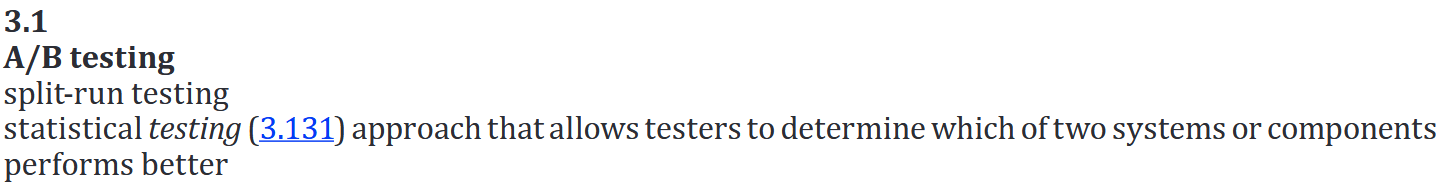
\includegraphics[width=\linewidth]{assets/images/a-b testing.png}
    \caption{\refHelper \citet[p.~1]{IEEE2022}'s glossary entry for
        ``A/B testing''.}\label{fig:IEEE-A-B-Testing}
\end{figure}
As we investigate other sources, we learn more about this approach. \refHelper
\citet[p.~58]{Firesmith2015} gives it as a child of usability testing, so we
include this Parent alongside ``Statistical Testing'' without issue. However,
since usability testing is a test type \ifnotpaper
    (\citealp[pp.~22, 26\=/27]{IEEE2022}; \citeyear[pp.~7, 40, Tab.~A.1]{IEEE2021};
    implied by its quality; \citealp[p.~53]{Firesmith2015})\else
    \cite[pp.~22, 26\=/27]{IEEE2022}, \cite[pp.~7, 40, Tab.~A.1]{IEEE2021}\fi,
A/B testing may inherit this categorization. We document this by adding
``Type'' as a Category alongside ``Practice'' with the source
``inferred from usability testing'', causing it to be automatically detected as
an inferred flaw \ifnotpaper (see \Cref{auto-flaw-analysis}) and appear in
    \Cref{tab:infMultiCats}\else (details omitted for brevity)\fi.

We use similar procedures to track software qualities \ifnotpaper (see
    \Cref{qual-test}) \fi and supplementary terminology (either shared by
multiple approaches or too complicated to explain inline) in separate
glossaries with a similar format. This includes recording the name, definition,
and synonym(s) of these terms, as well as any precedence for a related test
type for a given software quality. For example, analyzability\footnote{
    This may be spelled ``analyzability'' \citep[p.~18]{IEEE2017} or
    ``analysability'' \citep{ISO_IEC2023a}; since this is a dialectal
    difference, we do not count this as a label flaw (see
    \Cref{label-flaw-def}).}, modifiability, modularity, reusability, and
testability are all subqualities of maintainability \ifnotpaper
    (\citealp{ISO_IEC2023a}; \citealp[Tab.~A.1]{IEEE2021};
    \citealp[p.~7\=/10]{SWEBOK2024}) \else
    \cite[p.~7\=/10]{SWEBOK2024}, \cite[Tab.~A.1]{IEEE2021},
    \cite{ISO_IEC2023a} \fi which has an associated test type
\ifnotpaper
    (\citealp[pp.~5, 22]{IEEE2022}; \citeyear[p.~38, Tab.~A.1]{IEEE2021})\else
    \cite[pp.~5, 22]{IEEE2022}, \cite[p.~38, Tab.~A.1]{IEEE2021}\fi. This sets
a ``precedent'' for each of these subqualities having its own associated test
type (e.g., reusability testing).

We use heuristics to guide this process for all three
glossaries to increase confidence that all terms are identified, paying
special attention to the following when investigating a new source:
\begin{itemize}
    \item glossaries and lists of terms,
    \item testing-related terms (e.g., terms containing ``test(ing)'',
          \ifnotpaper ``review(s)'', ``audit(s)'', \fi
          ``validation'', or ``verification''),
    \item terms that had emerged as part of already-discovered
          testing approaches, \emph{especially} those that were ambiguous
          or prompted further discussion (e.g., terms containing
          ``performance'', ``recovery'', ``component'', ``bottom-up'',
          \ifnotpaper ``boundary'', \fi or ``configuration''), and
    \item terms that implied testing approaches%
          \ifnotpaper\footnote{
                  Since these methods for deriving test approaches only arose
                  as research progressed, some examples would have been missed
                  during the first pass(es) of resources investigated earlier
                  in the process. While reiterating over them would be ideal,
                  this may not be possible due to time constraints.
              } (see \Cref{derived-tests})\fi.
\end{itemize}
We apply these heuristics to most investigated sources, especially established
standards (see \Cref{stds}), in their entirety. Some sources, however, are only
partially investigated, such as those chosen for a specific area of
interest or based on a test approach that was determined to be out-of-scope.
These include the following sources as described in \Cref{undef-terms}:
\citep{ISO2022,ISO2015,Dominguez-PumarEtAl2020,PierreEtAl2017,
    TrudnowskiEtAl2017,YuEtAl2011,Tsui2007,Goralski1999}.

During the first pass of data collection, we investigate and record all
terminology related to software testing. Some of these terms are less
applicable to test case automation---our original motivation---%
\ifnotpaper(such as static testing; see \Cref{static-test}%
\thesisissueref{39})\ \fi%
or quite broad\ifnotpaper\ (such as attacks; see \Cref{attacks}%
    \thesisissueref{55})\fi, so they will be omitted during future analysis.
\ifnotpaper
    Others are so vague that they do not provide any new, meaningful
    information. For example, the ``systematic determination of the extent to
    which an entity meets its specified criteria'' \citep[p.~167]{IEEE2017} is
    certainly relevant to testing software; while this definition of
    ``evaluation'' may be meaningful when defining software testing generally,
    it does not define a new approach or procedure and applies much more
    broadly than just to testing. We decided\thesisissueref{39,44,28} that the
    following terms are too vague to merit tracking in our glossaries or
    analyzing further:
    \begin{itemize}
        \item \textbf{Evaluation:} the ``systematic determination of the extent
              to which an entity meets its specified criteria''
              \citep[p.~167]{IEEE2017}
        \item \textbf{Product Analysis:} the ``process of evaluating a product by
              manual or automated means to determine if the product has certain
              characteristics'' \citep[p.~343]{IEEE2017}
        \item \textbf{Quality Audit:} ``a structured, independent process to
              determine if project activities comply with organizational and
              project policies, processes, and procedures'' \citep[p.~361]{IEEE2017}
              \todo{OG PMBOK}
        \item \textbf{Software Product Evaluation:} a ``technical operation that
              consists of producing an assessment of one or more characteristics
              of a software product according to a specified procedure''
              \citep[p.~424]{IEEE2017}
    \end{itemize}

    \phantomsection{}\label{infers}
    Throughout this process, information can be inferred from ``surface-level''
    analysis that follows straightforwardly but isn't explicitly stated by any
    source. Examples of this are large scale integration testing and legacy
    system integration testing, described by \citeauthor{Gerrard2000a} in
    \citeyearpar[p.~30]{Gerrard2000b} and (\citeyear[Tab.~2]{Gerrard2000a};
    \citeyear[Tab.~1]{Gerrard2000b}), respectively. While he never explicitly
    says so, it can be inferred that these approaches are children of
    integration testing and system integration testing, respectively.
    Although these data do not come from the literature, they are documented
    for completeness; inferred flaws are given in \Cref{infer-flaws}
    and inferred relations, if any, are included in \recFigs{}.
\fi

\subsubsection{Derived Test Approaches}
\label{derived-tests}

Throughout this research, we noticed many groups of test approaches that arise
from some underlying area of software (testing) knowledge. The legitimacy of
extrapolating new test approaches from these knowledge domains is heavily
implied by the literature, but not explicitly stated as a general rule. Regardless,
since the field of software is ever-evolving, it is crucial to be able to
adapt to, talk about, and understand new developments in software testing.
Bases for defining new test approaches suggested by the literature include
coverage metrics, software qualities, and attacks. These are meaningful
enough to merit analysis and are therefore in scope. Requirements may also
imply related test approaches, but this mainly results in test approaches
that would be out of scope. Other test approaches found in the literature
are derived from programming languages or other orthogonal test approaches,
but these are out of scope as this information is better captured by other
approaches.

\ifnotpaper
\paragraph{Coverage-driven Techniques}\label{cov-test}

Test techniques are able to ``identify test coverage items \dots{} and
derive corresponding test cases''
\ifnotpaper
    (\citealp[p.~11]{IEEE2022}; similar in \citeyear[p.~467]{IEEE2017})
\else
    \cite[p.~11]{IEEE2022} (similar in \cite[p.~467]{IEEE2017})
\fi
in a ``systematic'' way
\citeyearpar[p.~464]{IEEE2017}.
\ifnotpaper
    This allows for ``the coverage achieved by a specific test design
    technique'' to be calculated as a percentage of ``the number of test
    coverage items covered by executed test cases'' \citeyearpar[p.~30]{IEEE2021}.
    %     ``Coverage levels can range
    %     from 0\% to 100\%'' and may or may not include ``infeasible'' test coverage
    %     items, which are ``not \dots{} executable or [are] impossible to be covered by a
    %     test case'' \citetext{p.~30}. Perhaps more interestingly, the further
    %     implication is
    % \else
    %     This means
\fi % that
Therefore, a given coverage metric implies a test approach aimed to
maximize it. For example, path testing ``aims to execute all entry-to-exit
control flow paths in a \acs{sut}'s control flow graph'' \citep[p.~5-13]{SWEBOK2024},
thus maximizing the path coverage
\ifnotpaper
    \citep[see][Fig.~1\thesisissueref{63}]{SharmaEtAl2021}\else
    (see \cite[Fig.~1]{SharmaEtAl2021}\thesisissueref{63})\fi.

\paragraph{Quality-driven Types}\label{qual-test}

Since test types are ``focused on specific quality characteristics''
\ifnotpaper
    (\citealp[p.~15]{IEEE2022}; \citeyear[p.~7]{IEEE2021};
    \citeyear[p.~473]{IEEE2017}\todo{OG IEEE 2013})%
\else
    \cite[p.~15]{IEEE2022}, \cite[p.~7]{IEEE2021}, \cite[p.~473]{IEEE2017}%
\fi, they can be derived from software qualities: ``capabilit[ies] of
software product[s] to satisfy stated and implied needs when used under
specified conditions'' \citep[p.~424]{IEEE2017}\todo{OG ISO/IEC 2014}. This
is supported by reliability and performance testing, which are both examples of
test types \citep{IEEE2022, IEEE2021} that are based on their underlying
qualities \citep[p.~18]{FentonAndPfleeger1997}.
% \ifnotpaper
%     For quantifying quality-driven testing, measurements should include
%     an entity to be measured, a specific attribute to measure, and the actual
%     measure (i.e., units, starting state, ending state, what to include)
%     \citetext{p.~36} where attributes must be
%     defined before they can be measured \citetext{p.~38}.
%
% \fi
Given the importance of software qualities to defining test types, the
definitions of \qualityCount{} software qualities are also tracked in this
current work\thesisissueref{21,23,27}. This was done by capturing their
definitions, any precedent for the existence of an associated test type,
and any synonyms (see \Cref{syn-rels}) and additional notes in a glossary.
We then ``upgrade'' software qualities to test types when they are mentioned
(or implied) by a source by removing its entry from this quality glossary
and adding an associated test approach to \ourApproachGlossary{} (as outlined
in \Cref{procedure}). Examples of this include conformance testing \ifnotpaper
    (\citealp[p.~5\=/7]{SWEBOK2024}; \citealp[p.~25]{JardEtAl1999}; implied
    by \citealp[p.~93]{IEEE2017})\else \cite[p.~5\=/7]{SWEBOK2024},
    \cite[p.~25]{JardEtAl1999}\fi, efficiency testing
\citep[p.~44]{Kam2008}, and survivability testing \citep[p.~40]{GhoshAndVoas1999}.

\paragraph{Attacks}\label{attacks}
While attacks can be ``malicious'' \citep[p.~7]{IEEE2017}, they are also
given as a test practice (\citeyear[p.~34]{IEEE2022}; see \Cref{tab:multiCats}).
This means that software attacks, such as code injection and password
cracking \citepISTQB{}, can also be used for testing software, and only
this kind of software attack is in scope. This is supported by the fact
that penetration testing is also called ``ethical hacking testing''
\citep[p.~13-4]{SWEBOK2024} or just ``ethical hacking''
\citep[p.~28]{Gerrard2000b}; while hacking in general is not a test
approach, doing so systematically to test and improve the software is.

\paragraph{Requirements-driven Approaches}\label{req-test}
While not as universally applicable, some types of requirements have associated
types of testing (e.g., functional, non-functional, security). This may mean
that categories of requirements \emph{also} imply related testing approaches
(such as ``technical testing''). \ifnotpaper Even assuming this is the case, some types of
    requirements do not apply to the code itself, and as such are out of scope%
    \thesisissueref{43}, such as:
    \begin{itemize}
        \item \textbf{Nontechnical Requirement:} a ``requirement affecting product
              and service acquisition or development that is not a property of
              the product or service'' \citep[p.~293]{IEEE2017}
        \item \textbf{Physical Requirement:} a ``requirement that specifies a
              physical characteristic that a system or system component must
              possess'' \citep[p.~322]{IEEE2017}
    \end{itemize}
\fi

\paragraph{Language-specific Approaches}\label{lang-test}
Specific programming languages are sometimes used to define test approaches.
If the reliance on a specific programming language is intentional, then
this really implies an underlying test approach that may be generalized to
other languages. These are therefore considered out-of-scope\thesisissueref{63},
including the following examples:

\begin{itemize}
    \item ``An approach \dots{} for JavaScript testing
          (referred to as Randomized)'' \citep[p.~192]{DoğanEtAl2014} is
          really just random testing used within JavaScript.
    \item ``SQL statement coverage'' is really just statement coverage
          used specifically for SQL statements \citep[Tab.~13]{DoğanEtAl2014}%
          \todo{OG Alalfi et al., 2010}.
    \item Testing for ``faults specific to PHP'' is just a subcategory of
          fault-based testing, since ``execution failures \dots{} caused by
          missing an included file, wrong MySQL quer[ies] and uncaught
          exceptions'' are not exclusive to PHP
          \citep[Tab.~27]{DoğanEtAl2014}\todo{OG Artzi et al., 2008}.
    \item While ``HTML testing'' is listed or implied by
          \citeauthor{Gerrard2000a} (\citeyear[Tab.~2]{Gerrard2000a};
          \citeyear[Tab.~1, p.~3]{Gerrard2000b}) and
          \citet[p.~220]{Patton2006}, it seems to be a combination of syntax
          testing, functionality testing, hyperlink testing/link checking,
          cross-browser compatibility testing, performance testing,
          content checking \citep[p.~3]{Gerrard2000b}, and grey-box testing
          \citep[pp.~218\==220]{Patton2006}.
\end{itemize}

\paragraph{Orthogonally Derived Approaches}\label{orth-test}
Some test approaches appear to be combinations of other (seemingly
orthogonal) approaches. While the use of a combination term can sometimes
make sense, such as when writing a paper or performing testing that focuses
on the intersection between two test approaches, they are sometimes given
the same ``weight'' as their atomic counterparts. For example, \citetISTQB{}
\multiAuthHelper{include} ``formal reviews'' and ``informal reviews'' in
\ifnotpaper their \else its \fi glossary as separate terms, despite their
definitions essentially boiling down to ``reviews that follow (or do not
follow) a formal process'', which do not provide any new information.
If a source describes an orthogonally derived approach in more detail, such
as security audits, we record it as a distinct approach in
\ourApproachGlossary{} with its related information. Otherwise, we consider
it out of scope since its details are captured by its in-scope subapproaches.
The following are examples of these out-of-scope orthogonally derived approaches:
% , with their subapproaches omitted for brevity as they 
% (which are apparent from the name of each ``combination approach''):

\begin{enumerate}
    \item Black box conformance testing \citep[p.~25]{JardEtAl1999}
          %   (combining black box and conformance testing)
          % Specification-based: Technique (IEEE, 2022, p. 22; 2021, p. 8; Washizaki, 2024, p. 5-10; Hamburg and Mogyorodi, 2024; Souza et al., 2017, p. 3; Firesmith, 2015, pp. 46-47; Sakamoto et al., 2013, p. 344; implied by IEEE, 2022, pp. 2-4, 6-9)
          % Conformance: Type (implied by its quality (IEEE, 2017, p. 92; OG PMBOK 5th ed.))
    \item Black-box integration testing \citep[pp.~345\==346]{SakamotoEtAl2013}
          % Specification-based: Technique (IEEE, 2022, p. 22; 2021, p. 8; Washizaki, 2024, p. 5-10; Hamburg and Mogyorodi, 2024; Souza et al., 2017, p. 3; Firesmith, 2015, pp. 46-47; Sakamoto et al., 2013, p. 344; implied by IEEE, 2022, pp. 2-4, 6-9)
          % Integration: Level (IEEE, 2022, pp. 12, 20-22, 26-27; 2021, p. 6; Washizaki, 2024, p. 5-7; Hamburg and Mogyorodi, 2024; Sakamoto et al., 2013, p. 343; Peters and Pedrycz, 2000, Tab. 12.3; van Vliet, 2000, p. 438; implied by Barbosa et al., 2006, p. 3)
          %           OR Technique (implied by Sharma et al., 2021, pp. 601, 603, 605-606)
    \item Checklist-based reviews \citepISTQB{}
          % Checklist-based: Practice (IEEE, 2022, p. 34), Technique (Hamburg and Mogyorodi, 2024)
          % Reviews: Approach
    \item Closed-loop HiL verification \citep[p.~6]{PreußeEtAl2012}
          % Closed Loop: Technique?
          % HiL: Out of Scope (hardware)
    \item Closed-loop protection system testing \citep[p.~331]{ForsythEtAl2004}
          % Closed Loop: Technique?
          % System: Level (IEEE, 2022, pp. 12, 20-22, 26-27; 2021, p. 6; 2017, p. 467; 2016, p. 4; Washizaki, 2024, p. 5-7; Hamburg and Mogyorodi, 2024; Sakamoto et al., 2013, p. 343; Peters and Pedrycz, 2000, Tab. 12.3; van Vliet, 2000, p. 439; implied by Barbosa et al., 2006, p. 3; Gerrard, 2000a, p. 13)
    \item Endurance stability testing \citep[p.~55]{Firesmith2015}
          % Endurance: Type (IEEE, 2013, p. 2; implied by Firesmith, 2015, p. 55)
          %         OR Technique (IEEE, 2021, p. 38)
          % Stability: Type (implied by its quality (IEEE, 2017, p. 434; OG ISO/IEC, 2009) and Firesmith, 2015, p. 55)
    \item End-to-end functionality testing (\citealp[p.~20]{IEEE2021}; \citealp[Tab.~2]{Gerrard2000a})
          % End-to-end: Type (Hamburg and Mogyorodi, 2024)
          %          OR Technique (Firesmith, 2015, p. 47; Sharma et al., 2021, pp. 601, 603, 605-606)
          % Functionality: Type (implied by its quality (IEEE, 2017, p. 196); Firesmith, 2015, p. 53)
    \item Formal reviews \citepISTQB{}
          % Formal: Technique (inferred from informal testing)
          % Reviews: Approach
    \item Grey-box integration testing \citep[p.~344]{SakamotoEtAl2013}
          % Grey-Box: Technique (IEEE, 2021, p. 8; Firesmith, 2015, pp. 46, 48; Sakamoto et al., 2013, p. 344)
          % Integration: Level (IEEE, 2022, pp. 12, 20-22, 26-27; 2021, p. 6; Washizaki, 2024, p. 5-7; Hamburg and Mogyorodi, 2024; Sakamoto et al., 2013, p. 343; Peters and Pedrycz, 2000, Tab. 12.3; van Vliet, 2000, p. 438; implied by Barbosa et al., 2006, p. 3)
          %           OR Technique (implied by Sharma et al., 2021, pp. 601, 603, 605-606)
    \item Incremental integration testing \citep[pp.~601, 603, 605\==606]{SharmaEtAl2021}\todo{OG [19]}
          % Incremental: Practice?
          % Integration: Level (IEEE, 2022, pp. 12, 20-22, 26-27; 2021, p. 6; Washizaki, 2024, p. 5-7; Hamburg and Mogyorodi, 2024; Sakamoto et al., 2013, p. 343; Peters and Pedrycz, 2000, Tab. 12.3; van Vliet, 2000, p. 438; implied by Barbosa et al., 2006, p. 3)
          %           OR Technique (implied by Sharma et al., 2021, pp. 601, 603, 605-606)
    \item Informal reviews \citepISTQB{}
          % Informal: Technique (implied by Kam, 2008, p. 6)
          % Reviews: Approach
    \item Infrastructure compatibility testing \citep[p.~53]{Firesmith2015}
          % Infrastructure: Type (implied by Firesmith, 2015, p. 57)
          %              OR Level (implied by Gerrard, 2000a, p. 13; see \Cref{tab:ieeeCats})
          % Compatibility: Type (IEEE, 2022, pp. 3, 22; 2021, p. 37, Tab. A.1; 2013, p. 2; implied by its quality (ISO/IEC, 2023a); Firesmith, 2015, p. 53)
    \item Invariant-based automatic testing \citep[pp.~184\==185, Tab.~21]{DoğanEtAl2014},
          including for ``AJAX user interfaces'' \citetext{p.~191}
          % Assertion Checking: Practice?
          % Automated: Practice (IEEE, 2022, pp. 20, 22)
          %         OR Technique (implied by p. 35)
    \item Legacy system integration (testing) \citep[Tab.~2]{Gerrard2000a}
          % Legacy: Approach
          % System Integration: Level (IEEE, 2022, pp. 12, 22; 2021, p. 6; Hamburg and Mogyorodi, 2024)
    \item Manual procedure testing \citep[p.~47]{Firesmith2015}
          % Manual: Practice (IEEE, 2022, p. 22)
          %      OR Technique (implied by p. 35)
          % Procedure: Type (IEEE, 2022, pp. 7, 22; 2021, p. 39, Tab. A.1; 2017, p. 337; OG IEEE, 2013)
          %         OR Technique (implied by Firesmith, 2015, p. 47)
    \item Manual security audits \citep[p.~28]{Gerrard2000b}
          % Manual: Practice (IEEE, 2022, p. 22)
          %      OR Technique (implied by p. 35)
          % Security Audits: Technique (IEEE, 2021, p. 40)
          %               OR Type (inferred from security testing)
    \item Model-based GUI testing (\citealp[Tab.~1]{DoğanEtAl2014}; implied by \citealp[p.~356]{SakamotoEtAl2013})
          % Model-based: Practice (IEEE, 2022, p. 22; 2021, p. viii)
          %           OR Technique (Engström and Petersen, 2015, pp. 1-2; Kam, 2008, p. 4; implied by IEEE, 2022, p. 32; 2021, p. 7; 2017, p. 469)
          % GUI: Approach
    \item Model-based web application testing (implied by \citealp[p.~356]{SakamotoEtAl2013})
          % Model-based: Practice (IEEE, 2022, p. 22; 2021, p. viii)
          %           OR Technique (Engström and Petersen, 2015, pp. 1-2; Kam, 2008, p. 4; implied by IEEE, 2022, p. 32; 2021, p. 7; 2017, p. 469)
          % Web Application: Approach
    \item Non-functional search-based testing \citep[Tab.~1]{DoğanEtAl2014}
          % Non-functional: Approach
          % Search-based: Technique (Engström and Petersen, 2015, pp. 1-2)
    \item Offline MBT \citepISTQB{}
          % Offline: Practice?
          % Model-based: Practice (IEEE, 2022, p. 22; 2021, p. viii)
          %           OR Technique (Engström and Petersen, 2015, pp. 1-2; Kam, 2008, p. 4; implied by IEEE, 2022, p. 32; 2021, p. 7; 2017, p. 469)
    \item Online MBT \citepISTQB{}
          % Online: Practice?
          % Model-based: Practice (IEEE, 2022, p. 22; 2021, p. viii)
          %           OR Technique (Engström and Petersen, 2015, pp. 1-2; Kam, 2008, p. 4; implied by IEEE, 2022, p. 32; 2021, p. 7; 2017, p. 469)
    \item Role-based reviews \citepISTQB{}
          % Role-based: Practice?
          % Reviews: Approach
    \item Scenario walkthroughs \citep[Fig.~4]{Gerrard2000a}
          % Scenario: Technique (IEEE, 2022, pp. 9, 22; 2021, pp. 5, 8, 20, Fig. 2; 2017, p. 400; OG 2013; Washizaki, 2024, p. 5-12; Firesmith, 2015, p. 47; Sangwan and LaPlante, 2006, p. 26)
          % Walkthroughs: Technique (IEEE, 2017, p. 508)
    \item Scenario-based reviews \citepISTQB{}
          % Scenario-based: Approach
          % Reviews: Approach
    \item Security attacks \citepISTQB{}
          % Security: Type (IEEE, 2022, pp. 9, 22, 26-27; 2021, pp. 7, 40, Tab. A.1; 2017, p. 405; OG 2013; implied by its quality (ISO/IEC, 2023a; Washizaki, 2024, p. 13-4); Firesmith, 2015, p. 53)
          % Attacks: Practice (IEEE, 2022, p. 34)
          %       OR Technique (implied by Hamburg and Mogyorodi, 2024)
    \item Security audits (\citealp[p.~40]{IEEE2021}; \citealp[p.~28]{Gerrard2000b})
          % Security: Type (IEEE, 2022, pp. 9, 22, 26-27; 2021, pp. 7, 40, Tab. A.1; 2017, p. 405; OG 2013; implied by its quality (ISO/IEC, 2023a; Washizaki, 2024, p. 13-4); Firesmith, 2015, p. 53)
          % Audits: Practice?
    \item Statistical web testing \citep[p.~185]{DoğanEtAl2014}
          % Statistical: Technique (Kam, 2008, pp. 23, 48)      
          % Web Application: Approach
    \item Usability test script(ing) \citepISTQB{}
          % Usability: Type (IEEE, 2022, pp. 22, 26-27; 2021, pp. 7, 40, Tab. A.1; implied by its quality; Firesmith, 2015, p. 53)
          % Scripted: Practice (IEEE, 2022, pp. 20, 22; implied by p. 33)
    \item Web application regression testing \cite[Tab.~21]{DoğanEtAl2014}
          % Web Application: Approach
          % Regression: Technique (implied by IEEE, 2022, p. 35)
          %          OR Level (implied by Barbosa et al., 2006, p. 3)
    \item White-box unit testing \citep[pp.~345\==346]{SakamotoEtAl2013}
          % Structure-based: Technique (IEEE, 2022, p. 22; 2021, p. 8; Washizaki, 2024, pp. 5-10, 5-13; Hamburg and Mogyorodi, 2024; Firesmith, 2015, pp. 46, 49; Sakamoto et al., 2013, p. 344; implied by IEEE, 2022, pp. 2, 4, 6, 9; Barbosa et al., 2006, p. 3)
          % Unit: Level (IEEE, 2022, pp. 12, 20-22, 26-27; 2021, p. 6; 2017, p. 467; 2016, p. 4; Washizaki, 2024, p. 5-6; Hamburg and Mogyorodi, 2024; Sakamoto et al., 2013, p. 343; Peters and Pedrycz, 2000, Tab. 12.3; van Vliet, 2000, p. 438; implied by Barbosa et al., 2006, p. 3)
          %    OR Technique (implied by Engström and Petersen, 2015, pp. 1-2)
\end{enumerate}

The existence of orthogonal combinations could allow for other test
approaches to be extrapolated from them. For example, \citet{Moghadam2019}
uses the phrase ``machine learning-assisted performance testing''; since
performance testing is a known test approach, we can infer the existence
of the test approach ``machine learning-assisted testing''. Likewise,
\citet{JardEtAl1999} \multiAuthHelper{use} the phrases ``local synchronous
testing'' and ``remote asynchronous testing''. While these can be
decomposed, for example, into local testing and synchronous testing,
the two resulting approaches may not be orthogonal, potentially even having
a parent-child relation (defined in \Cref{par-chd-rels}).

Based on their definitions and usage, the categories given in
\Cref{tab:ieeeCats} seem to be orthogonal. For example, ``a test type can be
performed at a single test level or across several test levels''
\ifnotpaper
    (\citealp[p.~15]{IEEE2022}; \citeyear[p.~7]{IEEE2021})%
\else
    \cite[p.~15]{IEEE2022}, \cite[p.~7]{IEEE2021}%
\fi, and ``Keyword-Driven Testing can be applied at all testing levels
\dots{} and for various types of testing'' \citeyearpar[p.~4]{IEEE2016}.
Therefore, we assume these categories to be orthogonal throughout this
\docType{} (e.g., when identifying flaws). We may assess this assumption more
rigorously in the future, but for now, it
implies that a specific test approach can be derived by combining multiple
test approaches from different categories. For example, usability test
script(ing) \citepISTQB{} is a combination of usability testing, a test type
\ifnotpaper (\citealp[pp.~22, 26--27]{IEEE2022};
    \citeyear[pp.~7, 40, Tab.~A.1]{IEEE2021}; implied by its quality;
    \citealp[p.~53]{Firesmith2015})\else \cite[pp.~22, 26--27]{IEEE2022},
    \cite[pp.~7, 40, Tab.~A.1]{IEEE2021}\fi, and scripted testing, a test
practice \citep[pp.~20, 22\ifnotpaper; implied by p.~33\fi]{IEEE2022}.

There are some cases where the subapproaches of the ``compound'' approaches
listed previously are \emph{not} from separate categories. However, these cases
can be explained by insufficient data or by edge cases that require special care.
While we assume that the categories given in \Cref{tab:ieeeCats} are
orthogonal, further analysis may disprove this. For now, all of these special
cases are affected by at least one of the following conditions:
\begin{enumerate}
    \item \textbf{At least one subapproach is categorized inconsistently.}
          When a subapproach has more than one category (see \Cref{multiCats}),
          it is unclear which one should be used to assess orthogonality.
    \item \textbf{At least one subapproach's category is inferred.} When the category
          of a test approach is not given by the literature but is inferred
          from related context (see \Cref{infers}), it is unclear if it can
          be used to assess orthogonality.
    \item \textbf{At least one subapproach is only categorized as an approach.}
          Since ``approach'' is a catch-all categorization, it does not
          need to be orthogonal to its subcategories.
    \item \textbf{A subapproach is explicitly based on another in the same
              category.} An example of this is stability testing, which
          tests a ``property that an object has with respect to a given
          failure mode if it cannot exhibit that failure mode''
          \citep[p.~434\todo{OG ISO/IEC, 2009}]{IEEE2017}. This notion of
          ``property'' is similar to that of ``quality'' that the test type
          category is built on, so it is acceptable that is implied to be
          a test type by its quality \citep[p.~434]{IEEE2017}%
          \todo{OG ISO/IEC, 2009} and by \citet[p.~55]{Firesmith2015}.
\end{enumerate}
\fi

\subsubsection{Undefined Terms}
\label{undef-terms}

The literature mentions many software testing terms without defining them.
While this includes test approaches, software qualities, and more general
software terms, we focus on the former as the main focus of our research.
In particular, many undefined test approaches are given by \ifnotpaper
    \citep{IEEE2022} and \citep{Firesmith2015}\else
    \cite{Firesmith2015} and \cite{IEEE2022}\fi. Once we exhaust the standards
in \Cref{stds}, we
perform miniature literature reviews on these subsets to ``fill in'' the
missing definitions (along with any relations), essentially ``snowballing''
on these terms. This process uncovers even more approaches, although some are
out of scope, such as \acf{emsec} testing\ifnotpaper, \else\ and \fi
aspects of \acf{orthat} \ifnotpaper and loop testing (see \Cref{hard-test}),
    and HTML testing (see \Cref{lang-test})\else (see \Cref{scope})\fi. The
following terms (and their respective related terms) were explored in the
sources given:
\input{build/undefTerms}
Applying our procedure from \Cref{procedure} to these sources brings the number
of testing approaches from \the\TotalBefore{} to \the\TotalAfter{} and the
number of \emph{undefined} terms from \the\UndefBefore{} to \the\UndefAfter{}%
\ifnotpaper\ (see \Cref{fig:undefPies})\fi. This implies that about
\the\numexpr 100 - 100 * (\UndefAfter - \UndefBefore) / (\TotalAfter -
\TotalBefore)\relax\% of added test approaches are defined, which helps verify
that our procedure constructively uncovers new terminology.

\ifnotpaper
    \begin{figure*}[hbtp!]
    \begin{subfigure}[c]{0.35\linewidth}
        \centering
        \begin{tikzpicture}[thick, scale=0.7, every label/.style={align=left, scale=0.7}]
            \pie[text=inside, sum=auto, color={blue!60, orange!60}]{
                {\the\numexpr \TotalBefore - \UndefBefore\relax}/,
                {\the\UndefBefore}/
            }
        \end{tikzpicture}
        \caption{The \the\TotalBefore{} approaches before investigating undefined terms.}
        \label{fig:undefPiesBefore}
    \end{subfigure}
    \hfill
    \begin{subfigure}[c]{0.35\linewidth}
        \centering
        \begin{tikzpicture}[thick, scale=0.7, every label/.style={align=left, scale=0.7}]
            \pie[text=inside, sum=auto, color={blue!60, orange!60}]{
                {\the\numexpr \TotalAfter - \UndefAfter\relax}/,
                {\the\UndefAfter}/
            }
        \end{tikzpicture}
        \caption{The \the\TotalAfter{} approaches after investigating undefined terms.}
        \label{fig:undefPiesAfter}
    \end{subfigure}
    \hfill
    \begin{subfigure}[c]{0.2\linewidth}
        \centering
        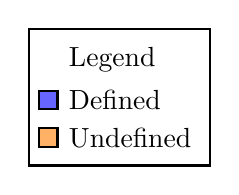
\begin{tikzpicture}
            \matrix [thick, draw=black] {
            \node[label=right:{Legend}] {}; \\
            \node[thick, shape=rectangle, draw=black, fill=blue!60,   label=right:{Defined}](0) {}; \\
            \node[thick, shape=rectangle, draw=black, fill=orange!60, label=right:{Undefined}](1) {}; \\
            };
        \end{tikzpicture}
    \end{subfigure}
    \caption{Breakdown of how many test approaches are undefined.}
    \label{fig:undefPies}
\end{figure*}

\fi

\phantomsection{}\label{missingTerms}
In addition to terms with missing definitions, some terms do not appear in
the literature at all! While most test approaches arise as a result of our
snowballing approach, we each have preexisting knowledge of what test
approaches exist (a form of experience-based testing, if you will).
As an example, we are surprised that property-based testing is not mentioned
in any sources investigated, even using it as a target ``stopping point''
throughout this process\thesisissueref{57,81,88,125}\qtodo{I think these issue
    refs, along with some others may actually be worth keeping in our final
    thesis/paper; thoughts?}. Test approaches such as these that arise
independently of snowballing may serve as starting points for continuing
research if they are not mentioned by the literature. The following terms come
from previous knowledge, conversations with colleagues, research for other
projects, or ad hoc cursory research to see what other test approaches exist:
\newline

\begin{minipage}{\linewidth}
    \begin{multicols}{2}
        \begin{enumerate}
            \item Chaos engineering
            \item Chosen-ciphertext \ifnotpaper\else \\ \fi attacks
            \item Concolic testing
            \item Concurrent testing
            \item Destructive testing
            \item Dogfooding
            \item Implementation-based testing
            \item Interaction-based \ifnotpaper\else \\ \fi testing
                  \ifnotpaper\else\columnbreak\fi
            \item Lunchtime attacks\ifnotpaper%
                      \footnote{In previous meetings, Dr.~Smith mentioned
                          that with the number of test approaches that suggest
                          that people just like to label everything as
                          ``testing'', he would not be surprised if something
                          like ``Monday morning testing'' existed. While
                          independently researching chosen-ciphertext attacks
                          out of curiosity, this prediction of a time-based
                          test approach came true with ``lunchtime attacks''.}
                  \fi
            \item Parallel testing
            \item Property-based testing
            \item Pseudo-random bit \ifnotpaper\else \\ \fi testing
            \item Rubber duck testing
            \item Scream testing
            \item Shadow testing
            \item Situational testing
        \end{enumerate}
    \end{multicols}
\end{minipage}

\ifnotpaper\section{Tools}
\else\subsection{Tools}
\fi\label{tools}

\ifnotpaper
    To better understand our findings, we build tools to
    visualize relations between test approaches (\Cref{app-rel-vis}) and
    automatically analyze their flaws (\Cref{flaw-analysis}). Doing
    this manually would be daunting and error-prone due to the amount of
    data involved (for example, we identify \approachCount{} test approaches).
    There are also many situations where the underlying data would change, such
    as adding to it, further analyzing it, or correcting it. % These all require
    % tedious updates to the corresponding visualizations that may be overlooked
    % or done incorrectly, so automating these processes allows for our results
    % to be reproduced (by us or others) and account for new data.
    % Besides being more systematic, automation also allows us to observe the
    % impacts of smaller changes, such as unexpected flaws that arise from a
    % new relation between two approaches. It also helps us verify the tools
    % themselves; for example, tracking a flaw manually should affect relevant
    % flaw counts, which we can double-check.
    We also define \LaTeX{} macros (\Cref{macros}) to help achieve our
    goals of maintainability, traceability, and reproducibility.

    \subsection{Approach Relation Visualization}\label{app-rel-vis}
\else
    % Moved here to display nicely in paper
    \flawMnfstsTable{}
    \flawDmnsTable{}
\fi

To better understand the relations between test approaches, we develop a tool
to visualize them. \ifnotpaper%
    % We can describe these graphs formally as ordered triplets
    %     $G = (A, S, P)$, where:  % Format based on https://en.wikipedia.org/wiki/Graph_theory
    %     \begin{itemize}
    %         \item $T$ is the set of terms assigned to test approaches by the
    %               literature,
    %         \item $A \subseteq T$ is a subset of the \approachCount{} test
    %               approaches we record as rows in \ourApproachGlossary{} that
    %               function as the vertices of the graph,
    %         \item $S \subseteq \left\{ \{x, y\} \mid x, y \in T \,\textrm{ and }\,
    %                   (x \in A \,\textrm{ or }\, y \in A) \,\textrm{ and }\, x \neq y \right\}$
    %               is a subset of our identified synonym relations (defined
    %               in \Cref{syn-rels}) that function as edges, and
    %         \item $P \subseteq \left\{(x,y) \mid (x, y) \in A^2 \right\}$ is a
    %               subset of our identified parent-child relations (defined in
    %               \Cref{par-chd-rels}) that also function as edges.
    %     \end{itemize}
    Since we use a consistent format to track synonym and parent-child
    relations (defined in \Cref{syn-rels,par-chd-rels}, respectively)
    between approaches in \ourApproachGlossary{}, we can parse them
    systematically. For example, if the entries in \Cref{tab:exampleGlossary}
    appear, then their parent-child relations are visualized as
    shown in \Cref{fig:exampleGraph}. Overall, the parent-child relations
    between test approaches \emph{should} result in something resembling a
    hierarchy (or multiple discrete hierarchies), although this is not the case
    due to flaws in the literature (see \Cref{selfParDef}). Therefore, we
    visualize all parent-child relations as they are guaranteed to be
    significant.

    However, since each term is trivially a synonym of itself and there are many
    non-problematic synonyms that do not imply flaws (see \Cref{syn-rels}),
    we only visualize the synonym relations that may indicate flaws given in
    \Cref{relevantSyns}; i.e., intransitive synonyms and synonyms between
    independently defined approaches.
    \clearpage
    % makecell with new lines so VS Code doesn't freak out
\def\app{\makecell{Approach\\Category}}

\begin{table}[hbtp!]
    \centering
    % Duplication required because '\ourApproachGlossary{}' doesn't work in table of contents
    \caption[Selected entries from our test approach glossary with ``Notes'' column excluded for brevity.]%
    {Selected entries from \ourApproachGlossary{} with ``Notes'' column excluded for brevity.}
    \label{tab:approachGlossaryExcerpt}
    \begin{tabularx}{\linewidth}{|m{1.5cm}|>{\raggedright\arraybackslash}m{4.1cm}|>{\raggedright\arraybackslash}X|>{\raggedright\arraybackslash}m{7cm}|>{\raggedright\arraybackslash}m{3.5cm}|}
        \hline
        \thead{Name}               & \thead{\app}                                                                                                                   & \thead{Definition}                                                                                                                                   & \thead{Parent(s)}                                                                                                                                                                                                                 & \thead{Synonym(s)}                                                                                    \\
        \hline
        A/B Testing                & Practice \citep[p.~22]{IEEE2022}, Type (inferred from usability testing)                                                       & Testing ``that allows testers to determine which of two systems or components performs better'' \citep[pp.~1, 36]{IEEE2022}                          & Statistical Testing \citep[pp.~1, 36]{IEEE2022}, Usability Testing \citep[p.~58]{Firesmith2015}                                                                                                                                   & Split-Run Testing \citep[pp.~1, 36]{IEEE2022}                                                         \\[1.5cm]
        % All Combinations Testing   & Technique (\citealp[p.~22]{IEEE2022}; \citeyear[pp.~2, 16]{IEEE2021}; \citealp[p.~5\=/11]{SWEBOK2024})                           & Testing that covers ``all unique combinations of P-V pairs'' \citep[p.~16]{IEEE2021}                                                                 & Combinatorial Testing \citetext{\citealp[p.~22]{IEEE2022}; \citeyear[pp.~2, 16, Fig.~2]{IEEE2021}; \citealp[p.~5\=/11]{SWEBOK2024}}                                                                                                                                                                                                                                                                                        & ---                                                                                                   \\[1cm]
        Big-Bang Testing           & Technique \citep[pp.~601, 603, 605\==606]{SharmaEtAl2021}, Level (inferred from integration testing)                           & ``Testing in which \dots{} [components of a system] are combined all at once into an overall system, rather than in stages'' \citep[p.~45]{IEEE2017} & Integration Testing (\citealp[p.~45]{IEEE2017}; \citealp[p.~5\=/7]{SWEBOK2024}; \citealp[p.~603]{SharmaEtAl2021}; \citealp[p.~42]{Kam2008}; \citealp[p.~488, Tab.~12.8]{PetersAndPedrycz2000})                                    & Sometimes spelled without a hyphen \citep[p.~489]{PetersAndPedrycz2000}                               \\[1.5cm]
        Classification Tree Method & Technique (\citealp[p.~22]{IEEE2022}; \citeyear[pp.~2, 12, Fig.~2]{IEEE2021}; \citealpISTQB{}; \citealp[p.~47]{Firesmith2015}) & Testing ``based on exercising classes in a classification tree'' \citep[p.~2]{IEEE2021}                                                              & Specification-based Testing (\citealp[p.~22]{IEEE2022}; \citeyear[pp.~2, 12, Fig.~2]{IEEE2021}; \citealpISTQB{}; \citealp[p.~47]{Firesmith2015}), Model-based Testing (\citealp[p.~13]{IEEE2022}; \citeyear[pp.~6, 12]{IEEE2021}) & Classification Tree Technique \citepISTQB{}, Classification Tree Testing \citep[p.~47]{Firesmith2015} \\[1.5cm]
        % Data Flow Testing          & Technique (\citealp[p.~22]{IEEE2022}; \citeyear[pp.~3, 27]{IEEE2021}; \citealp[p.~5\=/13]{SWEBOK2024}; \citealp[p.~43]{Kam2008}) & A ``class of \dots{} techniques based on exercising definition-use pairs'' \citep[p.~3; similar on p.~27]{IEEE2021}                                  & Structure-based Testing (\citealp[p.~22]{IEEE2022}; \citeyear[pp.~3, 27, Fig.~2]{IEEE2021}; \citealp[p.~43]{Kam2008}), Control Flow Testing (\citeyear[p.~27]{IEEE2021}; implied by \citealp[p.~5\=/13]{SWEBOK2024}; \citealp[p.~101]{IEEE2017}), Model-based Testing (\citeyear[p.~27]{IEEE2021}; implied by \citealp[p.~179]{DoğanEtAl2014}), Web Application Testing (p. 179; can be in \citealp[pp.~16\==17]{Kam2008}) & ---                                                                                                   \\
        \hline
    \end{tabularx}
\end{table}
    \ExampleParChdGraphs{}
    \clearpage
\fi%
% For a given synonym pair to
% be captured by our methodology, at least one term will have its own row in its
% relevant glossary.
% We then decide whether to include or exclude the synonym
% pair from our generated graphs based on the following possible cases:
% \begin{enumerate}
%     % \item[1. (Excluded)] \phantomsection{}\label{syn-case-one}
%     %       \hfill \ifnotpaper
%     %           $\left\{ \{x, y\} \in S \mid x \in A \,\textrm{ xor }\, y \in A \right\}$
%     %       \fi \break
%     %       \textbf{Only one synonym has its own row.}
%     %       This is a ``typical'' synonym relation (see \Cref{syn-rels}) where
%     %       the terms are interchangeable. We \emph{could} include the synonym
%     %       as an alternate name inside the node of its partner, but we do not
%     %       want to clutter our graphs unnecessarily.
%     \item%[2. (Included)] \phantomsection{}\label{syn-case-two}
%           %   \hfill \ifnotpaper
%           %       $\left\{ \{x, y\} \in S \mid x, y \in A \right\}$
%           %   \fi \break
%           \textbf{Synonyms between approaches defined independently.}\hfill\break
%           If two separate approaches have their own definitions, nuances,
%           etc.~but are also labelled as synonyms, this may indicate that the
%           two terms are interchangeable and could be merged \emph{or} that
%           either their definitions or this synonym relation is incorrect.
%           % TODO: pretty hacky
%           % into one row, which would result in \hyperref[syn-case-one]{Case 1} above.
%     \item%[3. (Included)] \phantomsection{}\label{syn-case-three}
%           %   \hfill \ifnotpaper
%           %       $\left\{ \{x, z\}, \{y, z\} \in S \mid x, y \in A \,\textrm{ and }\,
%           %           z \notin A \right\}$
%           %   \fi \break
%           \textbf{Synonyms that violate transitivity.}\hfill\break
%           If two distinct approaches share a synonym, that implies that they
%           are synonyms themselves. If they are \emph{not}, one or more
%           relations may be incorrect or missing.
% \end{enumerate}
\ifnotpaper
    \noindent
    We deduce these conditions from the information we parse from our glossary.
    For example, if the entries in \Cref{tab:synExampleGlossary} appear, then
    they are visualized as shown in \Cref{fig:exampleSynGraph} (note that X
    does not appear since it is not defined independently and does not violate
    transitivity). If a test approach does not have one of these relations
    \emph{or} a parent-child relation, we call it an ``orphan'' approach
    (in constrast to the ``parent'' and ``child'' approaches defined in
    \Cref{par-chd-rels}) and exclude it from any visualizations in which it
    would otherwise appear.\qtodo{Is this OK to ``define'' ``orphan''
        approaches here? We don't use it frequently and it requires us to
        define our ``significant'' synonym relations first.}

    \input{build/synExampleGlossary.tex}
    \ExampleSynGraph{}

    \phantomsection{}\label{visExplicit}
    We also visualize the ``explicitness'' of information (defined in
    \Cref{explicitness}) by representing implicit approaches and relations
    with dashed lines (see \Cref{fig:exampleGraph,fig:exampleSynGraph}).
    If a relation is both explicit \emph{and} implicit, we only display the
    latter if its source tier is more credible than the former's (see
    \Cref{cred,source-tiers}). For example, if
    ``StdAuthor'' from \Cref{tab:synExampleGlossary} is the author of a
    standard, then we display the implicit relation from their
    document alongside the explicit one from ``Author'' as shown in
    \Cref{fig:exampleSynGraph}.
    % For example, only the explicit synonym relation between E and F
    % from \Cref{tab:exampleGlossary} appears in \Cref{fig:synExampleGraph}.
    Explicit approaches
    \emph{always} have solid lines, even if they are also implicit. We
    can also omit implicit approaches and relations from visualizations; for
    example, \Cref{fig:expExampleGraph} is the explicit version of
    \Cref{fig:exampleGraph}. %, and \Cref{fig:expSynGraph} likewise only
    % contains explicit approaches and synonym relations

    \clearpage
    We also colour each relation according to its source tier, which is
    possible because we cite all recorded relations as described in
    \Cref{citation-syntax}. Each source tier gets its own colour, which we label
    for each relevant source tier in a given visualization's legend
    (such as \Cref{fig:exampleSynGraph}), although we omit this
    colouring from \Cref{fig:exampleParChdGraphs,fig:exampleFlawGraphs} for
    clarity. We also only display the relation with the most credible source
    tier (except if there is a more credible implicit relation as we previously
    describe). Finally, we also colour inferences (see \Cref{infers}) grey and
    proposals (see \Cref{recs}) orange, such as in \recFigs{}.

\fi
These visualizations tend to be large, so it is often useful to focus on
specific subsets of them. \ifnotpaper For each approach category (defined in
    \Cref{cats-def}), we generate a visualization restricted to its approaches
    and the relations between them. We also generate a visualization of all static
    approaches along with the relations between them \emph{and} between a
    static approach and a dynamic approach. This static-focused visualization is
    notable because static testing is sometimes considered to be a separate
    approach category (see \flawref{static-test-flaw}). Since dynamic
    approaches are our primary focus (see \Cref{static-test}), we include them
    in this static visualization, colouring their nodes grey to distinguish them.
    %, as in \Cref{fig:staticExampleGraph}, 
    We can also \else We can \fi generate more focused visualizations from a
given subset of approaches, such as \ifnotpaper\else those in a selected
    approach category (defined in \Cref{cats-def}) or \fi those pertaining to
recovery testing. % or scalability.
% These areas are of particular note as we discuss their
% flaws in their own sections (\Cref{recov-flaw,scal-flaw}, respectively).
We use these visualizations to better understand the relations within these
subsets of approaches, but we can also update them based on
our recommendations \ifnotpaper in \Cref{recs} \fi by specifying sets of
approaches and relations to add or remove. % given \else; the latter are shown
% \fi in \Cref{fig:rec-graph-current,fig:scal-graph-current}, respectively.
% applying those given in \Cref{rec-test-rec,,scal-test-rec,,\ifnotpaper\else%
%         perf-test-rec\fi} results in the updated graphs in
% \Cref{fig:rec-graph-proposed,,fig:scal-graph-proposed,,\ifnotpaper\else%
%         fig:perf-graph\fi}, respectively.
% \ifnotpaper
% Recommendations can also be inherited; for example, we generate
% \Cref{fig:perf-graph} based on the modifications we apply to
% \Cref{fig:rec-graph-proposed,fig:scal-graph-proposed} and
% other changes from \Cref{perf-test-rec}. \fi
\ifnotpaper
    \subsection{Flaw Analysis}
\label{flaw-analysis}

In addition to analyzing specific flaws, it is also useful to examine them at
a higher level. We automate subsets of this task where applicable
(\Cref{auto-flaw-analysis}) and augment the remaining manual portion with
automated tools (\Cref{aug-flaw-analysis}). This gives us an overview of:
\begin{itemize}
    \item how many flaws there are,
    \item how responsible each source tier (see \Cref{sources}) is for these flaws,
    \item how obvious (or ``rigid''; see \Cref{rigidity}) these flaws are,
    \item how these flaws present themselves (see \Cref{flawMnfsts}), and
    \item in which knowledge domains these flaws occur (see \Cref{flawDmns}).
\end{itemize}

To understand where flaws exist in the literature, we group them based on the
source tier(s) responsible for them. Each flaw is then counted \emph{once} per
source tier if it appears within it \emph{and/or} between it and a more
``credible'' tier\footnote{If an inconsistency occurs between two source tiers
    and the more credible one is \emph{incorrect}, we instead count it as an
    inconsistency between it and ground truth, as described in
    \Cref{lower-ground-truth}.} (see \Cref{cred,sources}). This avoids
counting the same flaw
more than once for a given source tier\thesisissueref{83}, which would give the
number of \emph{occurrences} of all flaws instead of the more useful number of
flaws \emph{themselves}. The exception to this is \Cref{fig:flawBars}, which
counts the following sources of flaws separately:
\begin{enumerate}
    \item those that appear once in (or consistently throughout) a document
          (i.e., are ``self-contained'')\thesisissueref{137,138},
    \item those between two parts of a single document
          (i.e., internal conflicts)\thesisissueref{137,138},
    \item those between documents with the same set of authors, which includes
          \begin{enumerate}
              \item the various combinations of ISO, the \acf{iec}, and IEEE
                    shown in \Cref{fig:ieeeSourceSets} and
              \item the different versions of the \acfp{swebok}, which have
                    different editors \citep{SWEBOK2024,SWEBOK2014} but are
                    written by the same organization: the IEEE Computer Society
                    (\citealp{AboutSWEBOK}; see \Cref{metas}), and
          \end{enumerate}
    \item those within a single source tier.
\end{enumerate}
As before, these are not double counted, meaning that the maximum number of
counted flaws possible within a \emph{single} source tier in
\Cref{fig:flawBars} is four (one for each type). This only occurs if
there is an example of each flaw source that is \emph{not} ignored to
avoid double counting; for example, while a single flaw within a single
document would technically fulfill all four criteria, it would only be counted
once.

\begin{figure}[bt!]
    \centering
    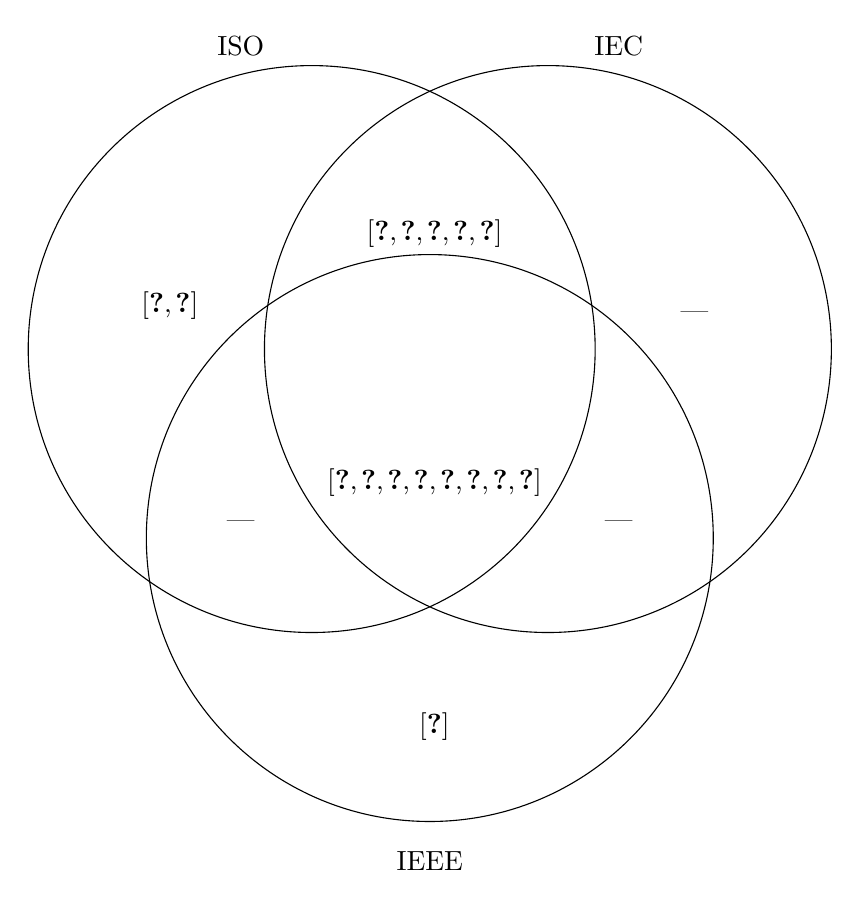
\begin{tikzpicture}
        \def\radius{3.6cm}
        \def\spread{1.5}
        \def\offset{\spread*1.6}

        \draw (-\spread, 0) circle (\radius);
        \draw ( \spread, 0) circle (\radius);
        \draw (0, -\offset) circle (\radius);

        \node[above] at (-\offset,        \radius) {ISO};
        \node[above] at ( \offset,        \radius) {IEC};
        \node[above] at (0, -\offset-1.85*\radius) {IEEE};

        % ALL
        \node[above] at (0, -\spread-0.5) {\parbox{3.7cm}{\centering
                \citealp{IEEE2022,IEEE2021,IEEE2019a,IEEE2019b,IEEE2017,
                    IEEE2016,IEEE2013,IEEE2010}}};
        % ISO/IEC
        \node[above] at (0, 0.325*\radius) {\parbox{2.8cm}{\centering
                \citealp{ISO_IEC2023a,ISO_IEC2023b,ISO_IEC2018,ISO_IEC2015,ISO_IEC2011}}};
        % ISO/IEEE
        \node[above] at ( \offset, -\offset) {---};
        % IEC/IEEE
        \node[above] at (-\offset, -\offset) {---};

        % ISO
        \node[above] at (-1.4*\offset, 0.25) {\parbox{2cm}{\centering
                \citealp{ISO2022,ISO2015}}};
        % IEC
        \node[above] at ( 1.4*\offset, 0.25) {---};
        % IEEE
        \node[above] at (0, -\spread-1.4*\radius) {\citealp{IEEE2012}};

    \end{tikzpicture}
    \caption{The sets of authors of established standards (see \Cref{stds}).}
    \label{fig:ieeeSourceSets}
\end{figure}

\phantomsection{}
\label{flaw-analysis-example}
As an example of this process, consider \flawref{level-phase-syns}, where an
IEEE standard has an internal flaw, and an inconsistency with two other IEEE
standards, and an inconsistency with a textbook. This adds one to the following
rows of \Cref{tab:flawMnfsts,tab:flawDmns} in the relevant column for a total
of two counted flaws:

\begin{itemize}
    \item \textbf{\stds{}}: this flaw occurs:
          \begin{enumerate}
              \item within one standard and
              \item between three standards (with the same set of authors).
          \end{enumerate}
          This increments the count by just one to avoid double counting and
          would do so even if only one of the above conditions was true. A more
          nuanced breakdown of flaws that identifies those within a
          singular document and those between documents by the same author is
          given in \Cref{fig:flawBars} and explained in more detail in
          \Cref{aug-flaw-analysis}; this view counts three total flaws here.
    \item \textbf{\texts{}}: this flaw occurs between a source in this tier and
          a ``more credible'' one (the IEEE standards; see \Cref{cred}).
          % \item \textbf{\papers{}}: this flaw occurs between a source in this tier
          %       and a ``more credible'' one. Even though there are two sources in this
          %       tier \emph{and} two ``more credible'' tier involved, this increments
          %       the count by just one to avoid double counting.
\end{itemize}

\subsubsection{Automated Flaw Analysis}
\label{auto-flaw-analysis}

As outlined in \Cref{graph-gen}, we automatically detect test approaches that
share a synonym (\hyperref[case-three]{Case 3} in \Cref{graph-gen}) to generate
our graphs. These relations are significant because they are potential flaws.
They arise from glossary entries such as those in \Cref{tab:synExampleGlossary}
which we automatically detect, format, and present in
\Cref{multiSyns,infMultiSyns}. The next logical step is to detect other classes
of flaws.\phantomsection{}\label{selfCycles}
The self-referential definitions in \Cref{selfPars} (defined as
$\left\{(x, y) \in P \mid x = y\right\}$) are also trivial to automate by
looking for lines in the
generated \LaTeX{} files that start with \texttt{I~->~I}, where \texttt{I}
is the label used for a test approach node in these graphs. This process
results in output similar to \Cref{fig:selfExampleGraph}. We use a similar
process to detect pairs of approaches with a synonym relation \emph{and} a
parent-child relation, defined as
$\left\{(x, y) \in P \mid \{x, y\} \in S\right\}$ and given in
\Cref{tab:parSyns,infParSyns}. To accomplish this, we build a dictionary of
each term's synonyms to evaluate which synonym relations are notable enough
to include in the graph, and then check these mappings to see if one appears
as a parent of the other. For example, if \texttt{J} and \texttt{K} are
synonyms, a generated \LaTeX{} file with a parent line starting with
\texttt{J~->~K} would result in these approaches being graphed as shown in
\Cref{fig:parSynExampleGraph}.

While just counting the total number of flaws (found automatically \emph{or}
manually) is trivial, tracking
the source(s) of these flaws is more useful, albeit more involved. Since
we consistently track the appropriate citations for each piece of information
we record (see \Cref{tab:exampleGlossary,tab:synExampleGlossary} for examples
of how these citations are formatted in the glossaries), we can use them to
identify the offending source tier(s). This comes with the added benefit that
we can format these citations to use with \LaTeX{}'s citation commands in this
\docType{}.

We compare the authors and years of each source involved with a given flaw
to determine if it manifests within a single document and/or between documents
with the same set of authors. Then, we group these sources into their tiers
\seeSrcCode{82167b7}{scripts/flawCounter.py}{63}{80}.
% done by the function in \Cref{lst:getSrcCat}, since each source tier
% outlined in \Cref{sources} is comprised of a small number of authors (with the
% exception of papers and other documents; see \Cref{papers}).
We then distill these lists of sources down to sets of tiers and compare them
against each other to determine how many times a given flaw manifests between
source tiers. This determines which row(s) of \Cref{tab:flawMnfsts,tab:flawDmns}
and which bar(s) of \Cref{fig:flawBars} that the given flaw should count toward.
We describe this process in more detail in \Cref{aug-flaw-analysis}.

\phantomsection{}
\label{auto-flaw-analysis-rigidity}
Alongside this citation information, we include keywords so we can assess how
``rigid'' a piece of information is (see \Cref{rigidity}). This is useful when
counting flaws, since they can be both explicit and implicit but should not be
double counted as both\thesisissueref{83}! When counting flaws in
\Cref{tab:flawMnfsts,tab:flawDmns}, each one is
counted only for its most ``rigid'' manifestation (i.e., it will only increment
a value in the ``Implicit'' column if it is \emph{not} also explicit),
similarly to how we generate graphs (see \Cref{graphRigid}).

\subsubsection{Augmented Flaw Analysis}
\label{aug-flaw-analysis}
While we can detect some subsets of flaws automatically by analyzing
\ourApproachGlossary, most are too complex and need to be tracked manually. We
record these more detailed flaws as \LaTeX{} enumeration items along with
comments that we can parse automatically, allowing us to analyze them more
broadly. We also add these comments to flaws we detect automatically before
generating the corresponding \LaTeX{} file to ensure these flaws also get
analyzed. These comments have the following format:
\begin{displayquote}
    \texttt{\% Flaw count (MNFST, DMN): \{A1\} \{A2\} \dots{} | \{B1\} % \{B2\}
        \dots{} | \{C1\} \dots}
\end{displayquote}
\texttt{MNFST} and \texttt{DMN} are placeholders for the ``keys'' given in
\Cref{tab:flawMnfstDefs,tab:flawDmnDefs}, respectively, that we use to track a
flaw's manifestation(s) and domain(s) (defined in \Cref{flaw-def}). We omit
these keys from constructed examples of these comments without associated flaws
throughout this chapter for brevity. Finally, \texttt{A1}, \texttt{A2}, % \texttt{B2},
\texttt{B1}, and \texttt{C1} are each placeholders for a source involved in
this example flaw; in general, there can be arbitrarily many. We represent each
source by its \BibTeX{} key, and wrap each one in curly braces (with the
exception of the \acs{istqb} glossary due to its use of custom commands via
\macro{citealias}) to mimic \LaTeX{}'s citation commands for ease of parsing.
We then separate each ``group'' of sources with a pipe symbol (\texttt{|}) so
we can compare each pair of groups; in general, a flaw can have any number of
groups of sources.

We make a distinction between ``self-contained'' flaws and ``internal'' flaws.
Self-contained flaws are those that manifest by comparing a document to a
source of ground truth. Sometimes, these do not require an explicit comparison;
for example, omissions (listed in \Cref{miss}) often fall into this category,
since the lack of information is contained within a single source and does not
need to be cross-checked against a source of ground truth. If only one group of
sources is present in a flaw's comment, such as the first line below, we
consider it to be a self-contained flaw. On the other hand, internal flaws
arise when a document disagrees with itself by containing two conflicting
pieces of information; this includes many contradictions and overlaps (listed
in \Cref{contra,over}, respectively). These can even occur on the same page,
such as when a source gives an acronym to two distinct terms
(see \flawref{cat-acro,hil-acro})! If a
source appears in multiple groups in a flaw's comment, we consider it to
be an internal flaw. The second line is a standard example of this, while the
third is more complex; in this case, source Y agrees with only one of the
conflicting sources of information in X.
\begin{displayquote}
    \texttt{\% Flaw count: \{X\}\\\% Flaw count: \{X\} | \{X\}\\
        \% Flaw count: \{X\} | \{X\} \{Y\}}
\end{displayquote}
We do not double count flaws that reappear when comparing between pairs of
groups; this means the following line adds an inconsistency between X and Z
\emph{and} between Y and Z \emph{without} double counting the former.
\begin{displayquote}
    \texttt{\% Flaw count: \{X\} | \{X\} \{Y\} | \{Z\}}
\end{displayquote}
To give a more complete example, we track \flawref{level-phase-syns} with the
following comment line:\utd{}
\begin{displayquote}
    \texttt{\% Flaw count (OVER, SYNS): \{IEEE2017\} \{IEEE2013\} | \{IEEE2022\}
        \displayNL{} \{IEEE2017\} \{Perry2006\}}
\end{displayquote}%
We parse this as the example given in \Cref{flaw-analysis-example}. Since
\texttt{IEEE2022}, \texttt{IEEE2017}, and \texttt{IEEE2013} are all written by
the same standards
organizations (\begin{NoHyper}\citeauthor{IEEE2022}\end{NoHyper}), we count
this as an inconsistency between documents with the same set of authors in
\Cref{fig:flawBars}, but only once to avoid double counting.

We can also specify the rigidity (see \Cref{rigidity}) of a flaw by inserting
the phrase ``implied by'' after the sources of explicit information and before
those of implicit information. This information is parsed following the same
rules described in \Cref{auto-flaw-analysis-rigidity} for automatically
detected flaws. Note that we only count implicit flaws if there is not an
equivalent explicit flaw, as we do when generating graphs (\Cref{graphRigid}).
\begin{displayquote}
    \texttt{\% Flaw count (CONTRA, DEFS): \{IEEE2021\} \{IEEE2017\} |
        \displayNL \{vanVliet2000\} implied by \{IEEE2021\}}
\end{displayquote}
For example, the above comment line\utd{} from \flawref{c-use-def} indicates
that the flaws given below are present. The third flaw only affects
\Cref{fig:flawBars} due to its more nuanced breakdown of the
sources of flaws. The rest increment their corresponding count in
\Cref{fig:flawBars,tab:flawMnfsts,tab:flawDmns} by only one:
\begin{itemize}
    \item an explicit inconsistency between a textbook and a standard,
    \item an implicit flaw within a single document, and
    \item an implicit inconsistency between documents with the same set of
          authors (\begin{NoHyper}\citeauthor{IEEE2022}\end{NoHyper}).
\end{itemize}

\phantomsection{}\label{lower-ground-truth}
Occasionally, we use a source from a lower tier as the ``ground truth'' for a
flaw. For example, \tolTestFlaw*{} This flaw is supported
by additional papers found via a miniature literature review (described in
\Cref{undef-terms}) from a lower source tier than \citep{Firesmith2015}
(which is a terminology collection; see \Cref{sources}). However, this flaw
is really based in \citep{Firesmith2015} and not in these
additional papers, but this would be counted as a flaw in these papers if they
were included as detailed above. Therefore, we document these ``ground
truth'' sources separately to track them for traceability without incorrectly
counting flaws, such as the following for this specific example
(\flawref{ground-truth}):
\begin{displayquote}
    \texttt{\% Flaw count (WRONG, LABELS): \{Firesmith2015\}\\
        \% Ground truth: \{LiuEtAl2023\} \{MorgunEtAl1999\} \{HolleyEtAl1996\}
        \displayNL \{HoweAndJohnson1995\}}
\end{displayquote}

\subsection[LaTeX Commands]{\LaTeX{} Commands}\label{macros}
To improve maintainability, traceability, and reproducibility, we define
helper commands (also called ``macros'') for content that is prone to change
or used in multiple places. For example, we use Python scripts to calculate
values based on our glossaries and save them to files to be assigned to
corresponding \LaTeX{} macros. We use these throughout our documents instead of
manually updating these constantly changing values, which is prone to error.
\Cref{tab:macrosCalc} lists these macros, along with their current values and
descriptions of what they represent. Our Python scripts convert numbers to
their textual equivalents when necessary to follow IEEE guidelines.

\begin{longtblr}[
    note{a} = {Calculated in \LaTeX{} from source tier lists; see \Cref{text-macros}.},
    note{b} = {Alias for \texttt{\textbackslash totalFlawDmnBrkdwn\{13\}}; see \Cref{flawCounts}.},
    note{c} = {These macros are defined as counters to allow them to be used in
            calculations within \LaTeX{} (such as in \Cref{undef-terms,fig:undefPies}).},
    caption = {\LaTeX{} macros for calculated values.},
    label = {tab:macrosCalc}
    ]{
    colspec={|X[0.3,l,m]X[0.5,c,m]X[0.2,c,m]|},
    width = \linewidth, rowhead = 1
    }
    \hline
    \thead{Macro}                                   & \thead{What it Counts}        & \thead{Value}    \\
    \hline
    \macro{approachCount}                           & Identified test approaches    & \approachCount{} \\
    \macro{qualityCount}                            & Identified software qualities & \qualityCount{}  \\
    \macro{srcCount}\TblrNote{a}                    & Sources used in glossaries    & \srcCount{}      \\
    \macro{flawCount}\TblrNote{b}                   & Identified flaws              & \flawCount{}     \\
    \hline
    \macro{TotalBefore}\TblrNote{c}                 & Test approaches identified
    before process in \Cref{undef-terms}            & \the\TotalBefore{}                               \\
    \macro{UndefBefore}\TblrNote{c}                 & Undefined test approaches
    identified before process in \Cref{undef-terms} & \the\UndefBefore{}                               \\
    \macro{TotalAfter}\TblrNote{c}                  & Test approaches identified
    after process in \Cref{undef-terms}             & \the\TotalAfter{}                                \\
    \macro{UndefAfter}\TblrNote{c}                  & Undefined test approaches
    identified after process in \Cref{undef-terms}  & \the\UndefAfter{}                                \\
    \hline
    \macro{multiSynCount}                           & Terms given as synonyms for
    multiple discrete terms                         & \multiSynCount{}                                 \\
    \macro{parSynCount}                             & Pairs of test approaches
    with a child-parent \emph{and} synonym relation & \parSynCount{}                                   \\
    \macro{selfCycleCount}                          & Test approaches that are
    a parent of themselves                          & \selfCycleCount{}                                \\
    \hline
\end{longtblr}


\phantomsection{}\label{flawCounts}
Additionally, we count flaws based on their manifestation and domain, rigidity,
and source tier (defined in \Cref{flaw-def,rigidity,sources}, respectively).
For each source tier, we create two files that each include both levels of
rigidity: one for manifestations and one for domains. For example, flaws in
standards are saved to \texttt{build/stdFlawMnfstBrkdwn.tex} by manifestation%
% and \texttt{build/stdFlawDmnBrkdwn.tex} for domains
. We then assign these data to macros (such as \macro{stdFlawMnfstBrkdwn}) to
populate \Cref{tab:flawMnfsts,tab:flawDmns}. For example, we access the number
of explicit and implicit mistakes in standards by using
\macro[1]{stdFlawMnfstBrkdwn} and \macro[2]{stdFlawMnfstBrkdwn}, respectively.
We follow a similar process for tracking the total numbers of flaws; this
includes \macro[13]{totalFlawMnfstBrkdwn} and \macro[13]{totalFlawDmnBrkdwn}
which are identical and track the total number of identified flaws.

\phantomsection{}\label{text-macros}
Just as with calculated values, it is important that repeated text is updated
consistently, which we accomplish by defining more macros. Some of these are
generated by Python scripts in a similar fashion to calculated values, such as
those for flaw manifestations and domains in \Cref{tab:macrosSections} and the
lists of sources in each source tier. The latter are built by extracting all
sources cited in our three glossaries, categorizing, sorting, and formatting
them (including handling edge cases), and saving them to a file. These are then
assigned to \macro{stdSources}, \macro{metaSources}, \macro{textSources}, and
\macro{paperSources} and include:
\begin{enumerate}
    \item the source tier's name,
    \item the list of sources in the tier, and
    \item the number of sources in the tier.
\end{enumerate}
These are accessed by passing in the corresponding number in the above
enumeration (e.g., \macro[2]{paperSources}). We use the first value for the
subheadings in \Cref{sources}, the first two for \Cref{app-src-tiers} and the
third to build \Cref{fig:sourceSummary} and calculate \macro{srcCount}
(see \Cref{tab:macrosCalc}).
% We also define macros for well-defined sections in \Cref{tab:macrosSections}.

\afterpage{
    \begin{landscape}
        \begin{longtblr}[
    note{a} = {Defined in \Cref{mnfst-def}; we also define starred versions,
            such as \macro{wrong*} (\wrong*{}), that use the singular noun for
            use in \Cref{tab:flawMnfstDefs}.},
    note{b} = {Defined in \Cref{dmn-def}; we only include domains with their
            own section.},
    % we also define starred versions,
    % such as \macro{cats*} (\cats*{}), that use the singular noun.
    note{c} = {Defined in \Cref{source-tiers}.},
    note{d} = {We overwrite the primitive \TeX{} command \macro{over}
            % Source: https://tex.stackexchange.com/a/73825/192195
            since we do not otherwise use it.},
    % note{e} = {We define a starred version, \macro{papers*} (\papers*{}), to shorten the
    %         display name for use in tables.},
    caption = {\LaTeX{} macros for referencing well-defined sections.},
    label = {tab:macrosSections}
    ]{
    colspec={|Q[1.75cm,c,m]|Q[l,m]Q[r,m]|Q[l,m]Q[r,m]|Q[l,m]Q[r,m]|},
    row{1} = {halign=c},
    width = \textwidth, rowhead = 1
    }
    \hline
                     & \SetCell[c=2]{c} \thead{Flaw Manifestations\TblrNote{a}}  &             & \SetCell[c=2]{c} \thead{Flaw Domains\TblrNote{b}} &           & \SetCell[c=2]{c} \thead{Source Tiers\TblrNote{c}} &              \\
    \hline
    \SetCell[r=6]{c} \textbf{Macros                                                                                                                                                                                               \\
    (Values)}        & \macro{wrong}                                             & (\wrong{})  & \macro{cats}                                      & (\cats{}) & \macro{stds}                                      & (\stds{})    \\
                     & \macro{miss}                                              & (\miss{})   & \macro{syns}                                      & (\syns{}) & \macro{metas}                                     & (\metas{})   \\
                     & \macro{contra}                                            & (\contra{}) & \macro{pars}                                      & (\pars{}) & \macro{texts}                                     & (\texts{})   \\
                     & \macro{ambi}                                              & (\ambi{})   &                                                   &           & \macro{papers}                                    & (\papers{})  \\ %\TblrNote{e}                                              \\
                     & \macro{over}\TblrNote{d}                                  & (\over{})   &                                                   &           & \macro{papers*}                                   & (\papers*{}) \\
                     & \macro{redun}                                             & (\redun{})  &                                                   &           &                                                                  \\
    \hline
    \textbf{Used In} & \SetCell[c=2]{c} {\Cref{tab:flawMnfstDefs,tab:flawMnfsts}
        % \\ (in both thesis and paper)
    }                &
                     & \SetCell[c=2]{c} {\Cref{tab:flawDmnDefs,tab:flawDmns}
        % \\ (in both thesis and paper)
    }                &                                                           &
    \SetCell[c=2]{c} {
    \Cref{fig:sourceSummary,fig:flawBars,fig:flawBarsSummary,fig:normFlawBarsSummary}                                                                                                                                             \\
        \Cref{tab:flawMnfsts,tab:flawDmns}
        % \\ \Cref{flaw-analysis-example} (only \macro{stds} and \macro{texts})
    }                &                                                                                                                                                                                                            \\
    \hline
\end{longtblr}

    \end{landscape}}

However, we create most of these macros for reused text manually when we first
notice the reuse, including the source tier macros in \Cref{tab:macrosSections}.
Some of these macros account for context-specific formatting depending on how
they are used, such as capitalization. These tend to be less well-defined,
since they arise naturally from the writing process, so we omit these details
from the manually created text macros in \Cref{tab:macrosText}, which are
grouped based on the type of information they contain.

% With help from https://tex.stackexchange.com/a/40468/192195, https://tex.stackexchange.com/a/245663/192195, and Copliot
\newcommand\macroType[2]{\multirow[b]{#1}{*}{\adjustbox{minipage=\the\dimexpr 0.3cm * #1 \relax,rotate=90}{#2}}}
% \newcommand\macroType[2]{\multirow[c]{#1}{*}{\rotatebox[origin=c]{90}{#2}}}

\begin{longtblr}[
    note{a} = {Defined in \Cref{flaw-def}.},
    note{b} = {See \Cref{tab:macrosSections} for more details on how we use
            \macro{redunNote} alongside \macro{redun}.},
    caption = {\LaTeX{} macros for reused text.},
    label = {tab:macrosText}
    ]{
    colspec={|Q[c,m]Q[l,m]X[l,m]|},
    row{1} = {halign=c},
    width = \textwidth, rowhead = 1
    }
    \hline
    \thead{Type}             & \thead{Macro}               & \thead{Used in}                                             \\*
    \hline
    \macroType{12}{Flaws\TblrNote{a}}
                             & \macro{bugPattonFlaw}       & \Cref{intro} and \flawref{bug-patton}                       \\*
                             & \macro{alphaFlaw}           & \Cref{intro} and \flawref{alpha-def}                        \\*
                             & \macro{loadFlaw}            & \Cref{intro} and \flawref{load-def}                         \\*
                             & \macro{expBasedCatMain}     & \Cref{intro,multiCats}                                      \\*
                             & \macro{tourFlaw}            & \Cref{intro,flaws} and \flawref{tour-def}                   \\*
                             & \macro{redBoxFlaw}          & \Cref{explicitness,wrong} and \flawref{dubious-red-box-syn} \\*
                             & \macro{perfAsFamily}        & \Cref{method-family,classFamilyFlaw}                        \\*
                             & \macro{tolTestFlaw}         & \Cref{less-cred-assert,wrong} and \flawref{assert-truth}    \\*
                             & \macro{accelTolTest}        & \macro{tolTestFlaw} and \Cref{hard-test}                    \\*
                             & \macro{errorGuessFlaw}      & \Cref{wrong} and \flawref{error-guess}                      \\*
                             & \macro{parSheetTestFlaw}    & \Cref{wrong} and \flawref{par-sheet-test}                   \\*
                             & \macro{perfSecParFlaw}      & \flawref{perf-sec-par} and paper version of \Cref{pars}     \\
    \hline
    \macroType{7}{Footnotes} & \macro{ftrnote}             & \SetCell[r=3]{l} Thesis (automated) and paper (manual)
    versions of \Cref{tab:parSyns}                                                                                       \\*
                             & \macro{specfn}              &                                                             \\*
                             & \macro{ucstn}               &                                                             \\*
    \cline{2-3}              & \macro{redunNote}           & \macro{redun} and \Cref{tab:flawMnfstDefs}\TblrNote{b}      \\*
    \cline{2-3}              & \macro{notDefDistinctIEEE}  & \flawref{static-test-flaw} and \Cref{exist-tax}             \\*
                             & \macro{gerrardDistinctIEEE} & \Cref{tab:otherCategorizations} and
    \flawref{gerrard-distinct}                                                                                           \\*
                             & \macro{distinctIEEE}        & \macro{gerrardDistinctIEEE}, \macro{notDefDistinctIEEE},
    and \Cref{method-family,classFamilyFlaw}                                                                             \\
    \hline
    \macroType{3}{Links}     & \macro{ourApproachGlossary} &
    \Cref{tab:approachGlossaryExcerpt,explicitness,record-terms,imp-info,app-rel-vis,%
    auto-flaw-analysis,aug-flaw-analysis,oat-test-rec}                                                                   \\*
                             & \macro{seeSrcCode}          & \Cref{app-rel-vis,auto-flaw-analysis}                       \\*
    % paper-macros
                             & \macro{recFigs}             & \Cref{flaws,recs}                                           \\
    \hline
    \macroType{3}{RQs}       & \macro{rqatext}             & \SetCell[r=3]{l} \Cref{intro} and seminar slides            \\*
                             & \macro{rqbtext}             &                                                             \\*
                             & \macro{rqctext}             &                                                             \\
    \hline
    \macroType{12}{Misc.}    & \macro{supersAck}           & \nameref{acknowledgements} and seminar slides               \\*
                             & \macro{supers}              & \nameref{decl_aca_ach} and \macro{supersAck}                \\*
                             & \macro{highLvlScope}        & \Cref{scope-overview,stds}                                  \\*
                             & \macro{defRel}              & \Cref{syn-rels,par-chd-rels}                                \\*
                             & \macro{defLabelDistinct}    & \Cref{label-flaw-def,labels}                                \\*
                             & \macro{oneSrcDistinct}      & \Cref{one-src-flaws,aug-flaw-analysis}                      \\*
                             & \macro{approachFields}      & \Cref{explicitness,record-terms}                            \\*
                             & \macro{impKeywords}         & \Cref{explicitness,imp-info}                                \\*
                             & \macro{orthTestIntro}       & \Cref{infers,orth-test}                                     \\*
                             & \macro{listAllSrcs}         & \Cref{source-tiers,ident-sources}                           \\*
                             & \macro{addTextEx}           & \Cref{texts,ident-sources}                                  \\*
                             & \macro{displayNL}           &
    \Cref{app-rel-vis,aug-flaw-analysis}                                                                                 \\
    % paper-macros,tab:macrosPaper
    \hline
\end{longtblr}


\phantomsection{}\label{paper-macros}
In addition to this thesis, we also prepare a conference paper based on our
research. While we can reuse most content without modifying it, we need to
address the formatting differences between the two document types.
In general, we use the conditional \texttt{\textbackslash ifnotpaper} to allow
for manual distinctions between the two documents' formats using this basic
template:
\begin{displayquote}
    \texttt{\textbackslash ifnotpaper <thesis code> \textbackslash else <paper code> \textbackslash fi}
\end{displayquote}
We define the macros given in \Cref{tab:macrosPaper} for recurring edge cases
between formatting requirements for these document types, presented along with
example usages and renderings. Since this document is the thesis, we have to
hardcode some of the paper renderings, so they may not be perfectly accurate.

\def\refHelperEx{\refHelper \ifnotpaper \citet{IEEE2022}
    \else \defcitealias{IEEE2022}{16}[\citetalias{IEEE2022}]
    \fi \multiAuthHelper{form} the basis of this \docType{}.}

\begin{longtblr}[
    note{a} = {Section omitted for brevity.},
    caption = {\LaTeX{} macros for handling formatting differences between thesis and paper.},
    label = {tab:macrosPaper}
    ]{
    colspec={|Q[c,m]|X[l,m]|},
    column{1} = {font=\bfseries},
    width = \textwidth, rowhead = 1
    }
    \hline
    \thead{Context} & \thead{Displayed as}                                                \\
    \hline
    Code            & {\texttt{\macro{refHelper} \macro[IEEE2022]{citet}\
    \macro[form]{multiAuthHelper}} \displayNL\texttt{the basis of this \macro{docType}.}} \\*
    Thesis          & \refHelperEx{}                                                      \\*
    Paper           & {\notpaperfalse \refHelperEx{}}                                     \\
    \hline
    Code            & \macro[cat-acro]{flawref}                                           \\*
    Thesis          & \flawref{cat-acro}                                                  \\*
    Paper           & Section \hyperref[cat-acro]{III-B2}                                 \\
    \hline
    Code            & \macro{redun}                                                       \\*
    Thesis          & \redun{}                                                            \\*
    Paper           & Redundancies\TblrNote{a}                                            \\
    \hline
\end{longtblr}


The most common difference between the two document styles is how citations are
displayed. We use the \texttt{natbib} package for our thesis, but the IEEE
guidelines for paper submissions suggest the use of \texttt{cite}
\citep[p.~8]{Shell2015a}. For simplicity, we define aliases so we can reuse
text that includes a single citation
\seeSrcCode{0a2dcdf}{paper_preamble.tex}{19}{60}. However, text that
cites multiple sources requires more work to be reused and has to be done so
manually, since the \texttt{natbib} package groups multiple citations within a
single set of parentheses while the \texttt{cite} package keeps them separate
inside their own set of square brackets.

For example, in \Cref{nonIEEE-sources}, we provide a list of non-IEEE sources
that support a claim made by the IEEE. Since we sort sources based on
credibility (defined in \Cref{cred}) and then by publication year, the
relevant thesis code is given below. (We use ``\texttt{\textbackslash =/}'',
etc. from the \texttt{extdash} package for non-breaking dashes.)
\begin{displayquote}
    \texttt{(\textbackslash citealp[pp.\textasciitilde 5\textbackslash =/6 to 5\textbackslash =/7]\{SWEBOK2024\};
        \displayNL \textbackslash citealpISTQB\{\};
        \textbackslash citealp[pp.\textasciitilde 807\textbackslash ==808]\{Perry2006\};
        \displayNL \textbackslash citealp[pp.\textasciitilde 443\textbackslash ==445]\{PetersAndPedrycz2000\};
        \displayNL \textbackslash citealp[p.\textasciitilde 218]\{KuļešovsEtAl2013\}; %\textbackslash todo\{OG Black, 2009\};
        \displayNL \textbackslash citealp[pp.\textasciitilde 9, 13]\{Gerrard2000a\})}
\end{displayquote}
Meanwhile, IEEE guidelines recommend that references ``appear in the order in
which they are cited'' \citep[p.~1]{Shell2015b}. Therefore, the relevant paper
code for this list of sources is:
\begin{displayquote}
    \texttt{\textbackslash cite[pp.\textasciitilde 443\textbackslash ==445]\{PetersAndPedrycz2000\},
        \displayNL \textbackslash cite[pp.\textasciitilde 5\textbackslash =/6 to 5\textbackslash =/7]\{SWEBOK2024\},
        \textbackslash cite\{ISTQB\},
        \displayNL \textbackslash cite[pp.\textasciitilde 807\textbackslash ==808]\{Perry2006\},
        \displayNL \textbackslash cite[pp.\textasciitilde 9, 13]\{Gerrard2000a\},
        \displayNL \textbackslash cite[p.\textasciitilde 218]\{KuļešovsEtAl2013\}}
\end{displayquote}\utd{}In particular, note the usage of the \macro{cite}
command, the \emph{lack} of use of the custom alias for citing the \acs{istqb}
glossary, and the different ordering and punctuation.
% , and the lack of the \macro{todo}, since these are only rendered for
% reference in the thesis.

\else
    When doing so in \Cref{recs}, we colour any proposed approaches
    or relations orange to distinguish them.
\fi

\section{Observed Flaws}\label{flaws}

% Moved earlier to display nicely in paper
% \flawMnfstsTable{}
% \flawDmnsTable{}

After gathering all these data\footnote{Available in \texttt{ApproachGlossary.csv},
    \texttt{QualityGlossary.csv}, and \texttt{SuppGlossary.csv} at \ifblind{
        [Repository link suppressed]}{
        \url{https://github.com/samm82/TestingTesting}}.}, we find many
flaws. \Cref{fig:flawBars} shows the source tiers (see \Cref{source-tiers})
responsible for these flaws, which reveals a lot about software testing literature:
\begin{enumerate}
    \item Established standards (\Cref{stds}) aren't actually standardized, since:
          \begin{enumerate}
              \item other documents disagree with them \emph{very} frequently and
              \item they are the most internally inconsistent source tier!
          \end{enumerate}
    \item Less standardized (or ``credible''; see \Cref{cred}) documents,
          such as terminology collections and textbooks (\Cref{metas,texts},
          respectively) are also not followed to the extent they should be.
    \item Documents across the board have flaws within the same document,
          between documents with the same author(s), or even with reality%
          \qtodo{Is this too strong of a synonym for ``ground truth''?}!
\end{enumerate}

To better understand and analyze these flaws, we group them by their
manifestations and their domains as defined in \Cref{flaw-def}.
We present the total number of flaws by manifestation and by domain
in \Cref{tab:flawMnfsts,tab:flawDmns}, respectively, where a given
row corresponds to the number of flaws either within that source tier and/or
with a ``more credible'' one (i.e., a previous row in the table; see
\Cref{cred,source-tiers}). We also group these flaws by their explicitness
(defined in \Cref{explicitness}) by counting (Obj)ective and (Sub)jective flaws
separately, since additional context may rectify them.
Since we give each flaw a manifestation \emph{and} a domain, the totals per
source and grand totals in these tables are equal. From these tables, we can
draw some conclusions about \emph{how} the literature is flawed:
\begin{enumerate}
    \item Contradictions are by \emph{far} the most common way for a flaw to
          manifest, which makes sense: if two (groups of) authors do not
          communicate or work with different resources, there is a higher
          chance that they will disagree.
    \item Approach categorizations are the most subjective and one of the most
          common flaw domains, likely due to the lack of standardization
          about what categories to use\ifnotpaper\ (see \Cref{alt-cats}
              for more detailed discussion)\fi.
\end{enumerate}

\ifnotpaper
    \begin{figure}[bt!]
\centering
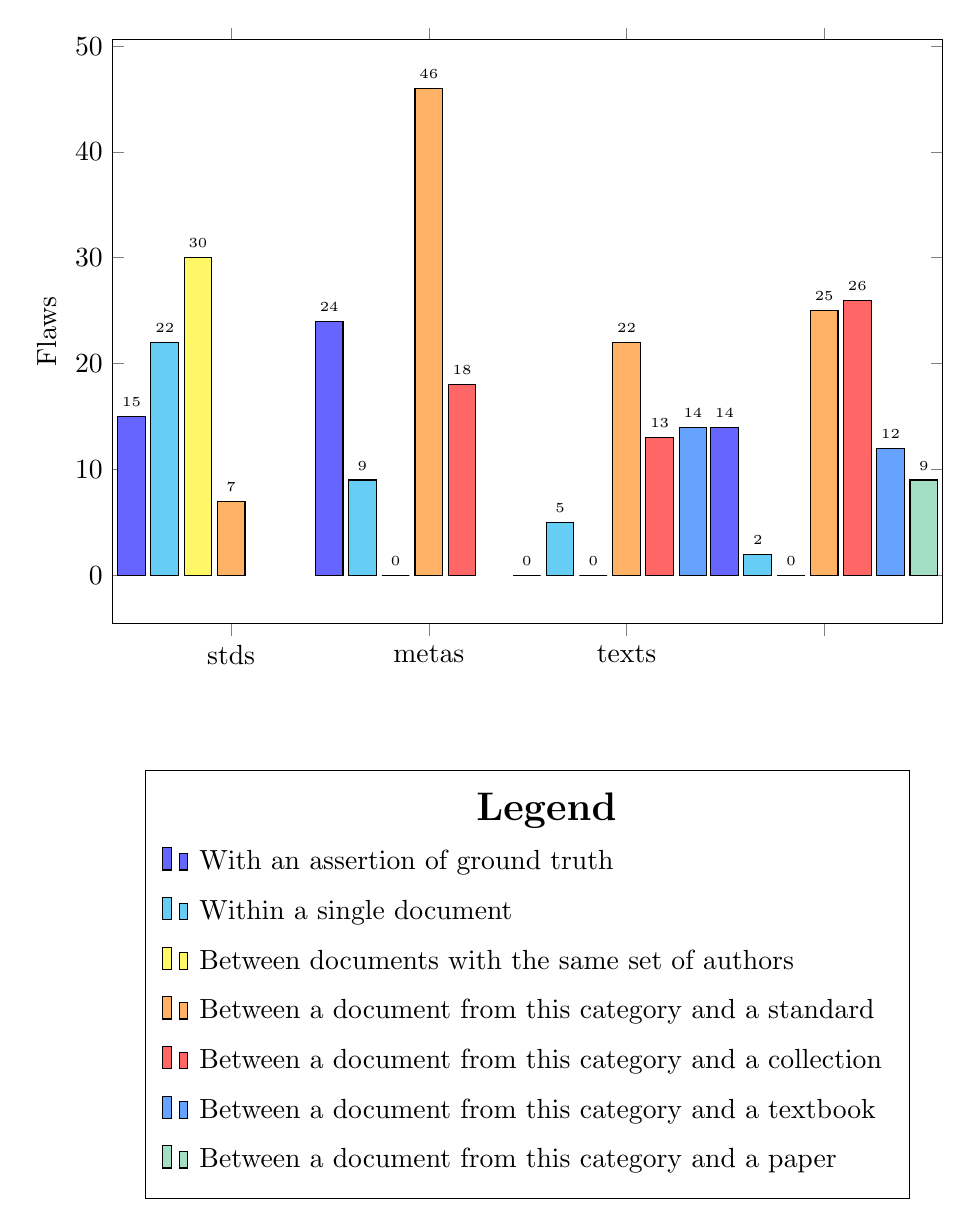
\begin{tikzpicture}
\begin{axis}[
width=\textwidth, height=9cm,
symbolic x coords={std,meta,text,paper},
xtick=data,
xticklabels={{\parbox{0.16\textwidth}{\centering \stds{}}},{\parbox{0.16\textwidth}{\centering \metas{}}},{\parbox{0.16\textwidth}{\centering \texts{}}},{\parbox{0.16\textwidth}{\centering \papers{}}}},
ylabel=Flaws, ybar,
enlargelimits=0.2, enlarge y limits=0.1,
legend style={at={(0.5,-0.25)}, anchor=north, legend columns=1,
inner xsep=6pt,inner ysep=4pt,
nodes={inner sep=4pt,text depth=0.3em},},
legend cell align=left,
nodes near coords,
every node near coord/.append style={font=\tiny},
]
\addlegendimage{empty legend}
\addplot[fill=blue!60] coordinates {(std, 15) (meta, 24) (text, 0) (paper, 14)};
\addplot[fill=cyan!60] coordinates {(std, 22) (meta, 9) (text, 5) (paper, 2)};
\addplot[fill=yellow!60] coordinates {(std, 30) (meta, 0) (text, 0) (paper, 0)};
\addplot[fill=orange!60] coordinates {(std, 7) (meta, 46) (text, 22) (paper, 25)};
\addplot[fill=red!60] coordinates {(meta, 18) (text, 13) (paper, 26)};
\addplot[fill=blue!60!cyan!60] coordinates {(text, 14) (paper, 12)};
\addplot[fill=cyan!60!yellow!60] coordinates {(paper, 9)};
\legend{\hspace{3.4cm} \Large \textbf{Legend},With an assertion of ground truth,Within a single document,Between documents with the same set of authors,Between a document from this category and a standard,Between a document from this category and a collection,Between a document from this category and a textbook,Between a document from this category and a paper}
\end{axis}
\end{tikzpicture}
\caption{Identified flaws by the source tier responsible. Some bars are omitted as they correspond to comparisons we do not make; see \Cref{flaw-cred-compare}.}
\label{fig:flawBars}
\end{figure}

    % \begin{figure*}
\centering
\begin{subfigure}[t]{0.475\textwidth}
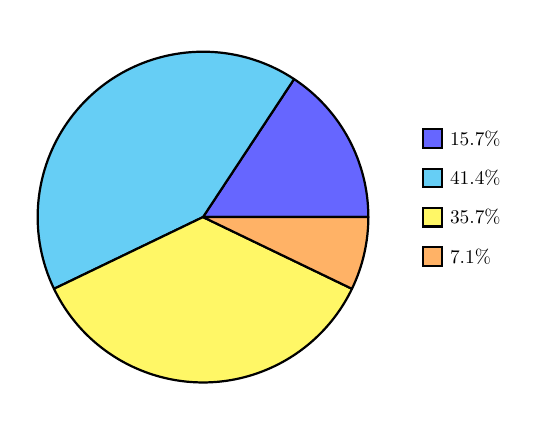
\begin{tikzpicture}[thick, scale=0.7, every label/.style={align=left, scale=0.7}]
   \pie[text=legend, sum=auto, hide number, color={blue!60, cyan!60, yellow!60, orange!60}]{
      11/15.7\%,
      29/41.4\%,
      25/35.7\%,
      5/7.1\%
}
\end{tikzpicture}
\caption{Flaws found in \stds{}.}
\label{fig:stdFlawSources}
\end{subfigure}
\hfill
\begin{subfigure}[t]{0.475\textwidth}
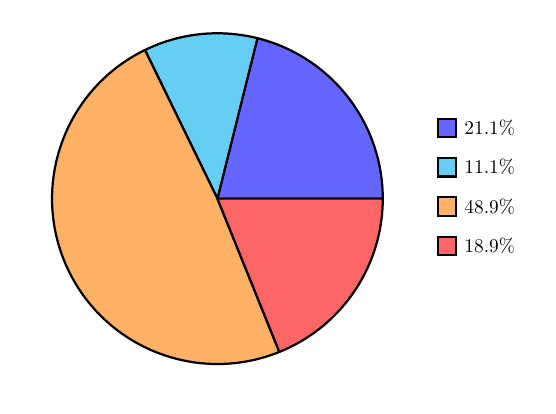
\begin{tikzpicture}[thick, scale=0.7, every label/.style={align=left, scale=0.7}]
   \pie[text=legend, sum=auto, hide number, color={blue!60, cyan!60, orange!60, red!60}]{
      19/21.1\%,
      10/11.1\%,
      44/48.9\%,
      17/18.9\%
}
\end{tikzpicture}
\caption{Flaws found in \metas{}.}
\label{fig:metaFlawSources}
\end{subfigure}
\vskip\baselineskip
\begin{subfigure}[t]{0.475\textwidth}
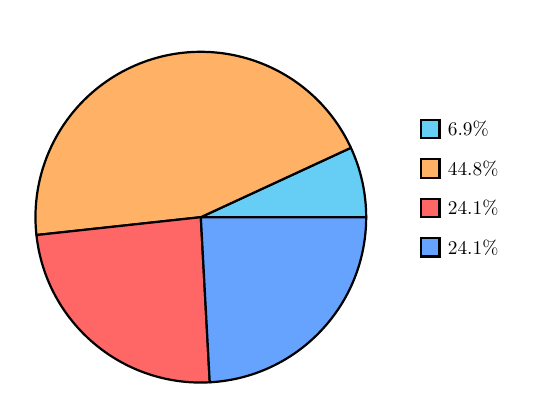
\begin{tikzpicture}[thick, scale=0.7, every label/.style={align=left, scale=0.7}]
   \pie[text=legend, sum=auto, hide number, color={cyan!60, orange!60, red!60, blue!60!cyan!60}]{
      4/6.9\%,
      26/44.8\%,
      14/24.1\%,
      14/24.1\%
}
\end{tikzpicture}
\caption{Flaws found in \texts{}.}
\label{fig:textFlawSources}
\end{subfigure}
\hfill
\begin{subfigure}[t]{0.475\textwidth}
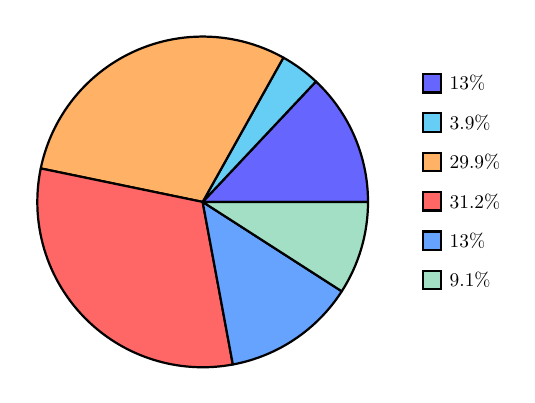
\begin{tikzpicture}[thick, scale=0.7, every label/.style={align=left, scale=0.7}]
   \pie[text=legend, sum=auto, hide number, color={blue!60, cyan!60, orange!60, red!60, blue!60!cyan!60, cyan!60!yellow!60}]{
      10/13\%,
      3/3.9\%,
      23/29.9\%,
      24/31.2\%,
      10/13\%,
      7/9.1\%
}
\end{tikzpicture}
\caption{Flaws found in \papers{}.}
\label{fig:paperFlawSources}
\end{subfigure}
\vskip\baselineskip
\begin{center}
\begin{subfigure}[t]{\linewidth}
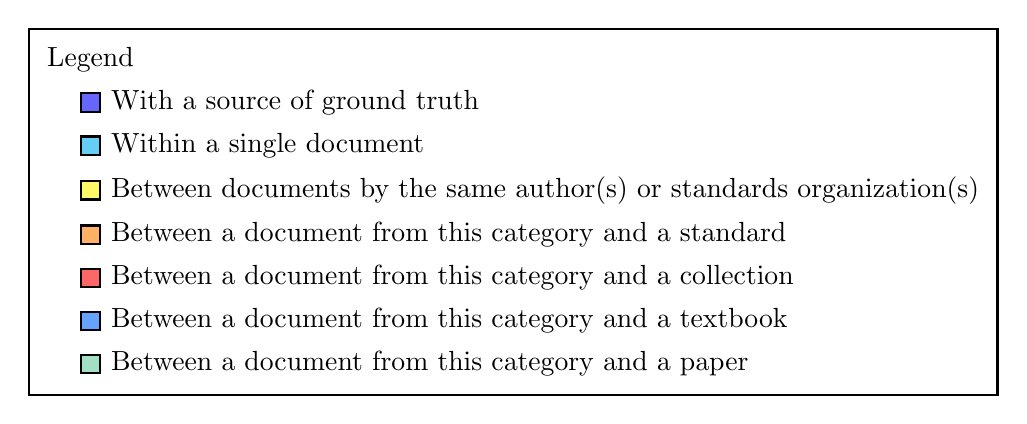
\begin{tikzpicture}
\matrix [thick, draw=black] {
\node[label=center:Legend] {{}}; \\
\node[thick, shape=rectangle, draw=black, fill=blue!60, label=right:{With a source of ground truth}](0) {}; \\
\node[thick, shape=rectangle, draw=black, fill=cyan!60, label=right:{Within a single document}](1) {}; \\
\node[thick, shape=rectangle, draw=black, fill=yellow!60, label=right:{Between documents by the same author(s) or standards organization(s)}](2) {}; \\
\node[thick, shape=rectangle, draw=black, fill=orange!60, label=right:{Between a document from this category and a standard}](3) {}; \\
\node[thick, shape=rectangle, draw=black, fill=red!60, label=right:{Between a document from this category and a collection}](4) {}; \\
\node[thick, shape=rectangle, draw=black, fill=blue!60!cyan!60, label=right:{Between a document from this category and a textbook}](5) {}; \\
\node[thick, shape=rectangle, draw=black, fill=cyan!60!yellow!60, label=right:{Between a document from this category and a paper}](6) {}; \\
};
\end{tikzpicture}
\end{subfigure}
\end{center}
\hfill
\caption{Sources of flaws based on \hyperref[sources]{source tier}.}
\label{fig:flawSources}
\end{figure*}


    % \input{build/flawTable}
    \begin{landscape}
        \flawMnfstsTable{}
        \flawDmnsTable{}
    \end{landscape}

\fi

We summarize the flaws that we discover manually \ifnotpaper (see
    \Cref{aug-flaw-analysis}) \fi in \Cref{flawMnfsts} based on their
manifestation (defined in \Cref{mnfst-def}). This lets us keep flaws that we
automatically uncover \ifnotpaper (see \Cref{auto-flaw-analysis}) \fi separate;
we summarize these based on their domain (defined in \Cref{dmn-def}) in
\Cref{flawDmns}.
\ifnotpaper We list \emph{all} these flaws in \Cref{flaws-full} to balance
    completeness and brevity and denote implicit relations with the phrase
    ``implied by'' in \Cref{tab:parSyns,tab:multiCats,tab:infMultiCats} as
    described in \Cref{explicitness}. \fi Moreover, certain ``subsets'' of
testing contain many interconnected flaws, which we present in subsections as a
``third view'' to keep related information together. Therefore, the counts of
flaws given in \Cref{tab:flawMnfsts,tab:flawDmns} can be thought of as the sum
the flaws we describe by manifestation, domain, and ``subset''. These subsets
include \ifnotpaper operational (acceptance) testing (\Cref{oat-flaw}), \fi
recovery testing (\Cref{recov-flaw}), scalability testing (\Cref{scal-flaw}),
and compatibility testing (\Cref{compat-flaw}). \ifnotpaper Finally, we also
    infer some flaws as described in \Cref{infers}, which do not contribute to
    any counts due to their subjectivity; we list them in \Cref{infer-flaws}
    for completeness. \fi

\subsection{Flaws by Manifestation}\label{flawMnfsts}

The following sections list observed flaws grouped by \emph{how} they manifest
as presented in \Cref{mnfst-def}. These include mistakes (\Cref{wrong}),
omissions (\Cref{miss}), contradictions (\Cref{contra}), ambiguities
(\Cref{ambi}), overlaps (\Cref{over}), and redundancies (\Cref{redun}).

\subsubsection{Mistakes}\label{wrong}

There are many ways that information can be incorrect which we identify in
\Cref{tab:brkdwnWrong}. We provide an example below for those that are less
straightforward\ifnotpaper; see \Cref{wrong-full} for the full list of
mistakes\fi.

\begin{table}[tb]
    \centering
    \begin{talltblr}[
        note{a} = {Comprises two typos and one duplication.},
        caption = {Different kinds of mistakes found in the literature.},
        label = {tab:brkdwnWrong}
        ]{
        colspec={|X[l,m]Q[c,m]|},
        width = \columnwidth, rowhead = 1
        }
        \hline
        \thead{Description}                                                & \thead{Count} \\
        \hline
        Information is incorrect based on an assertion from another source & 9             \\
        Information is not present where it is claimed to be               & 6             \\
        Information is provided with an incorrect scope                    & 5             \\
        Information contains a minor mistake                               & 3\TblrNote{a} \\
        Incorrect information makes other information incorrect            & 1             \\
        \hline
    \end{talltblr}
\end{table}


\paragraph{Information is incorrect based on an assertion from another source}
\errorGuessFlaw{}

\paragraph{Information is provided with an incorrect scope}
\parSheetTestFlaw{} Conversely, \tolTestFlaw*{}

\paragraph{Incorrect information makes other information incorrect}
\redBoxFlaw{}

\subsubsection{Omissions}\label{miss}
We find four cases where a definition is omitted and one where a category is
omitted \ifnotpaper which we list in \Cref{miss-full}\fi.

\subsubsection{Contradictions}\label{contra}
There are many cases where multiple sources of information (sometimes within
the same document!) disagree. We find this happen with six categories, five
synonym relations, seven parent-child relations, 18 definitions, and two
labels. \ifnotpaper These can be found in \Cref{contra-full}.\fi

\subsubsection{Ambiguities}\label{ambi}
Some information given in the literature is unclear; there is definitely
something ``wrong'', but we cannot deduce the intent of the original author(s).
We identify the kinds of ambiguous information given in \Cref{tab:brkdwnAmbi}%
\ifnotpaper; see \Cref{ambi-full} for the full list of ambiguities\fi.

\begin{table}[tb]
    \centering
    \begin{talltblr}[
        % note{a} = {Comprises two typos and one duplication.},
        caption = {Different kinds of ambiguities found in the literature.},
        label = {tab:brkdwnAmbi}
        ]{
        colspec={|X[l,m]Q[c,m]|},
        width = \columnwidth, rowhead = 1
        }
        \hline
        \thead{Description}                          & \thead{Count} \\
        \hline
        A term is ambiguously defined                & 9             \\
        A term is used inconsistently                & 2             \\
        The distinction between two terms is unclear & 2             \\
        A test approach is ambiguously categorized   & 1             \\
        \hline
    \end{talltblr}
\end{table}


\subsubsection{Overlaps}\label{over}
While information given in the literature should be atomic, this is not
always the case. We find three definitions that overlap, two terms with
multiple definitions, and three terms that share acronyms. \ifnotpaper We list
    these in \Cref{over-full}; note that we track two of the terms with
    multiple definitions as the same flaw since they are related. \fi

\subsubsection{Redundancies}\label{redun}
We find redundancies in two parent-child relations, one definition, and two
labels\ifnotpaper\ as listed in \Cref{redun-full}\fi.

\subsection{Flaws by Domain}\label{flawDmns}

The following sections present flaws that we detect automatically \ifnotpaper
    (see \Cref{auto-flaw-analysis}) \fi grouped by \emph{what} information
is flawed as presented in \Cref{dmn-def}. We also provide more detailed
information on specific areas of these domains that may require further
investigation. The domains we focus on here are test approach categories
(\Cref{cats}), synonym relations (\Cref{syns}), and parent-child relations
(\Cref{pars})%\ifnotpaper, and definitions (\Cref{defs})\fi
.

% Moved here to display nicely in paper
\ifnotpaper\else
    \begin{paperTable}
    \centering
    \caption{Test approaches with more than one category.}\label{tab:multiCats}
    \begin{minipage}{\linewidth}
        \centering
        \begin{tabular}{|r|l|l|}
            \hline
            \thead{Approach}         & \thead{Category 1}                                                  & \thead{Category 2}                                                                                                                              \\
            \hline
            Ad Hoc Testing           & Practice \cite[p.~33]{IEEE2013}                                     & Technique \cite[p.~5\=/14]{SWEBOK2024}                                                                                                          \\
            Capacity Testing         & Technique \cite[pp.~38\==39]{IEEE2021c}                             & Type \cite[p.~22]{IEEE2022}, \cite[p.~2]{IEEE2013}                                                                                              \\
            Checklist-based Testing  & Practice \cite[p.~34]{IEEE2022}                                     & Technique \cite{ISTQB}                                                                                                                          \\
            Data-driven Testing      & Practice \cite[p.~22]{IEEE2022}                                     & Technique \cite[p.~43]{Kam2008}                                                                                                                 \\
            End-to-end Testing       & Type \cite{ISTQB}                                                   & Technique \cite[p.~47]{Firesmith2015}, \cite[pp.~601, 603, 605\==606]{SharmaEtAl2021}                                                           \\
            Endurance Testing        & Technique \cite[pp.~38\==39]{IEEE2021c}                             & Type \cite[p.~2]{IEEE2013}                                                                                                                      \\
            %                                                                                                                                                   pp.~iii\==iv, 4, 11, 29, 35, 122, 125, 
            Error Guessing           & Practice \cite[p.~33]{IEEE2013}                                     & Technique \cite[pp.~4, 34, Fig.~2]{IEEE2022}, \cite[Fig.~2, Tab.~A.2]{IEEE2021c}\footnote{Some sources omitted for brevity.}                    \\ %, \cite[pp.~3, 33]{IEEE2013}, \cite[p.~5\=/13]{SWEBOK2024}, \cite[p.~50]{Firesmith2015} \\
            Experience-based Testing & Technique \cite[pp.~46, 50]{Firesmith2015}, \cite[Fig.~2]{IEEE2022} & Practice \cite[Fig.~2]{IEEE2022}, \cite[p.~viii]{IEEE2021c}, \cite[pp.~iii, 31, 33]{IEEE2013}                                                   \\
            %                                                                                                                                                                                                   TODO: remove footnote duplication
            Exploratory Testing      & Technique \cite[p.~50]{Firesmith2015}, \cite[p.~5\=/14]{SWEBOK2024} & Practice \cite[pp.~11, 20, 34, Fig.~2]{IEEE2022}, \cite[p.~viii]{IEEE2021c}, \cite[p.~5]{IEEE2021a}\footnote{Some sources omitted for brevity.} \\ %, \cite[pp.~13, 33]{IEEE2013} \\
            Load Testing             & Technique \cite[pp.~38\==39]{IEEE2021c}                             & Type \cite[p.~253]{IEEE2017}, \cite[pp.~5, 20, 22]{IEEE2022}, \cite{ISTQB}                                                                      \\
            Performance Testing      & Technique \cite[pp.~38\==39]{IEEE2021c}                             & Type \cite[pp.~7, 22, 26\==27]{IEEE2022}, \cite[p.~7]{IEEE2021c}, \cite[pp.~2, 8]{IEEE2021a}                                                    \\
            Stress Testing           & Technique \cite[pp.~38\==39]{IEEE2021c}                             & Type \cite[p.~442]{IEEE2017}, \cite[pp.~9, 22]{IEEE2022}                                                                                        \\
            \hline
        \end{tabular}
    \end{minipage}
\end{paperTable}

    \begin{paperTable}
    \centering
    \caption{Pairs of test approaches with both \hyperref[par-chd-rels]{parent-child} and \hyperref[syn-rels]{synonym} relations.}
    \label{tab:parSyns}
    \begin{minipage}{\linewidth}
        \centering
        \begin{tabular}{|rcl|l|l|}
            \hline
            \thead{``Child''}        & \thead{$\to$} & \thead{``Parent''}                              & \thead{Parent-Child Source(s)}                                        & \thead{Synonym Source(s)}                                                   \\
            \hline
            All Transitions Testing  & $\to$         & State Transition Testing                        & \citep[p.~19]{IEEE2021}                                               & \citep[p.~15]{Kam2008}                                                      \\
            Co-existence Testing     & $\to$         & Compatibility Testing                           & \cite[p.~3]{IEEE2022}, \cite[Tab.~A.1]{IEEE2021}, \cite{ISO_IEC2023a} & \citep[p.~37]{IEEE2021}                                                     \\
            Fault Tolerance Testing  & $\to$         & Robustness Testing\footnote{\ftrnote{}}         & \citep[p.~56]{Firesmith2015}                                          & \citepISTQB{}                                                               \\
            Functional Testing       & $\to$         & Specification-based Testing\footnote{\specfn{}} & \citep[p.~38]{IEEE2021}                                               & \cite[p.~196]{IEEE2017}, \cite[p.~399]{vanVliet2000}, \cite[p.~44]{Kam2008} \\
            Orthogonal Array Testing & $\to$         & Pairwise Testing                                & \citep[p.~1055]{Mandl1985}                                            & \cite[p.~5-11]{SWEBOK2024}, \cite[p.~473]{Valcheva2013}                     \\
            Path Testing             & $\to$         & Exhaustive Testing                              & \citep[pp.~466-467, 476]{PetersAndPedrycz2000}                        & \citep[p.~421]{vanVliet2000}                                                \\
            Performance Testing      & $\to$         & Performance-related Testing                     & \cite[p.~22]{IEEE2022}, \cite[p.~38]{IEEE2021}                        & \citep[p.~1187]{Moghadam2019}                                               \\
            Static Analysis          & $\to$         & Static Testing                                  & \cite[pp.~9, 17, 25, 28]{IEEE2022}, \cite{ISTQB}                      & \citep[p.~438]{PetersAndPedrycz2000}                                        \\
            % Omitted parent-child sources for static row :\cite[Fig.~4, p.~12]{Gerrard2000a}, \cite[p.~3]{Gerrard2000b}                                     
            Structural Testing       & $\to$         & Structure-based Testing                         & \citep[pp.~105\=/121]{Patton2006}                                     & \cite[p.~9]{IEEE2022}, \cite{ISTQB}, \cite[pp.~443\=/444]{IEEE2017}         \\
            Use Case Testing         & $\to$         & Scenario Testing\footnote{\ucstn{}}             & \cite[p.~20]{IEEE2021}\todo{OG Hass, 2008}                            & \cite{ISTQB}, \cite[pp.~47-49]{Kam2008}                                     \\
            \hline
        \end{tabular}
    \end{minipage}
\end{paperTable}

\fi

\subsubsection{Approach Category Flaws}\label{cats}

While the IEEE categorization of testing approaches described in
\Cref{tab:ieeeCats} is useful, it is not without its faults. One issue,
which is not inherent to the categorization itself, is the fact that it is not
used consistently\ifnotpaper\ (see \Cref{tab:otherCats})\fi. The most
blatant example of this is that \ifnotpaper \else \citeauthor{IEEE2017} \fi
\citet[p.~286]{IEEE2017} describe mutation testing as a
methodology, even though this is not one of the categories \emph{they} created!
% Flaw count (CONTRA, CATS): {IEEE2017} | {IEEE2022}
Additionally, the boundaries between approaches within a category may
be unclear: ``although each technique is defined independently of all others,
in practice [sic] some can be used in combination with other techniques''
\citep[p.~8]{IEEE2021c}. For example, ``the test coverage items derived by
applying equivalence partitioning can be used to identify the input parameters
of test cases derived for scenario testing'' \citetext{p.~8}. Even the categories
themselves are not consistently defined, and some approaches are categorized
differently by different sources; we track these differences so we can analyze
them more systematically\thesisissueref{21}.

\phantomsection{}\label{multiCats}
\ifnotpaper
    \begin{wraptable}{r}{6cm}
        \vspace{-0.75cm}
        \input{build/multiCatTable}
        \vspace{-1cm}
    \end{wraptable}
\fi
In particular, \multiCatIntro{}. We identify \multiCatCount{} such cases%
\ifnotpaper\ that we summarize in \Cref{tab:multiCatTable}\fi; we consider
these flaws as they violate our assumption of orthogonality (see
\Cref{orth-approach}). We list \ifnotpaper all \else some \fi of these flaws
along with their sources in \Cref{tab:multiCats}\ifnotpaper\ for completeness\fi.
These flaws mostly involve the category of ``test \multiCatMax{}'', which
shows up in \multiCatMaxCount{} of them. This may simply be because authors use
the term ``test technique'' in a more general sense where we would use the term
``test approach''.\phantomsection{}\label{cats-intrans} A more
specific reason for this is how the line between ``test technique'' and
``test practice'' can be blurred when these categories are \emph{not}
transitive. For example, ``some test practices, such as exploratory testing or
model-based testing are sometimes [incorrectly] referred to as `test techniques'
\dots{} as they are not themselves providing a way to create test cases, but
instead use test design techniques to achieve that'' \ifnotpaper
    (\citealp[p.~11]{IEEE2022}; \citeyear[p.~5]{IEEE2021a})\else
    \cite[p.~11]{IEEE2022}, \cite[p.~5]{IEEE2021a}\fi. This seems to be the
case for the following approaches, which may explain these apparent ``flaws'':
\begin{itemize}
    \item Exploratory testing \ifnotpaper (\citeyear[p.~33]{IEEE2022};
              \citeyear[p.~viii]{IEEE2021c}; \citeyear[p.~13]{IEEE2013}) \else
              \cite[p.~33]{IEEE2022}, \cite[p.~viii]{IEEE2021c},
              \cite[p.~13]{IEEE2013} \fi
    \item Experience-based testing \ifnotpaper (\citeyear[p.~4]{IEEE2022};
              \citeyear[pp.~viii, 4]{IEEE2021c}; \citeyear[p.~33]{IEEE2013})
          \else \cite[p.~4]{IEEE2022}, \cite[pp.~viii, 4]{IEEE2021c},
              \cite[p.~33]{IEEE2013} \fi
    \item Scripted testing \citeyearpar[p.~33]{IEEE2022} \ifnotpaper
    \item Ad hoc testing (\citealp[p.~5\=/14]{SWEBOK2024}; \citealpISTQB{};
          \citealp[p.~42]{Kam2008})
    \item Model-based testing (\citealp[pp.~1\==2]{EngströmAndPetersen2015};
          \citealp[p.~4]{Kam2008}) \fi
\end{itemize}

\ifnotpaper
    As described in \Cref{infers}, we infer that child approaches inherit their
    parents' categories. However, there seem to be exceptions to this, which
    may indicate that categories are \emph{not} transitive or that they are
    \emph{except} in certain cases. For example, the practice of experience-based
    testing has many subtechniques, as described above, but it \emph{also} has
    subpractices, including tours \citep[p.~34]{IEEE2022} and exploratory testing
    (although the latter is categorized inconsistently; see \Cref{tab:multiCats}
    and above discussion). Similarly, the conflicting categorizations of beta
    testing in \Cref{tab:multiCats} may propagate to its children closed beta
    testing and open beta testing. When we infer these flaws, we exclude them
    from \Cref{tab:multiCatTable,tab:multiCats} and instead include them in
    \Cref{tab:infMultiCats} for completeness.
    \newpage
\fi

\subsubsection{Synonym Relation Flaws}\label{syns}

While synonyms do not inherently signify a flaw (as we discuss in
\Cref{syn-rels}), the software testing literature is full of incorrect and
ambiguous synonyms that do. As described in \Cref{relevantSyns}, we pay
special attention to synonyms between independently defined approaches (which
may be flaws) and to intransitive synonyms (which definitely \emph{are} flaws).
\ifnotpaper We present explicit (see \Cref{explicitness}) synonym relations that
    fit either of these criteria in \Cref{fig:expSynGraph}\utd{}, which we
    automatically generate from \ourApproachGlossary{} and manually modify for
    legibility. These relations are given as described by the literature and are
    therefore flawed. We provide the full list of synonyms that violate
    transitivity (along with their sources) in \Cref{multiSyns} and discuss and
    other kinds of flawed synonym relations in \Cref{parSyns,scal-flaw,compat-flaw}.
\fi

\subsubsection{Parent-Child Relation Flaws}\label{pars}
\phantomsection{}\label{selfPars}
Parent-child relations are also not immune to flaws. For example, some
approaches are given as parents of themselves which violates the
irreflexivity of this relation as defined in \Cref{par-chd-rels}.
% Since these are by nature self-contained within a given source, we count these
% \emph{once} as objective flaws within
% their sources in \Cref{tab:flawMnfsts,tab:flawDmns}.
\ifnotpaper We identify
    the following \selfParCount{} examples through automatic analysis of our
    generated graphs (see \Cref{selfParDef}):
    \input{build/selfPars} Interestingly, performance testing is \emph{not}
    described as a subapproach of usability testing by \citep{Gerrard2000a,
        Gerrard2000b}, which would have been more meaningful information to
    capture. \else For example, performance and usability testing are both
    given as subapproaches of themselves \cite[Tab.~2]{Gerrard2000a},
    \cite[Tab.~1]{Gerrard2000b}.\fi
% Flaw count (MISS, PARS): {Gerrard2000a} {Gerrard2000b}

\ifnotpaper
    \begin{figure}[bt!]
        \centering
        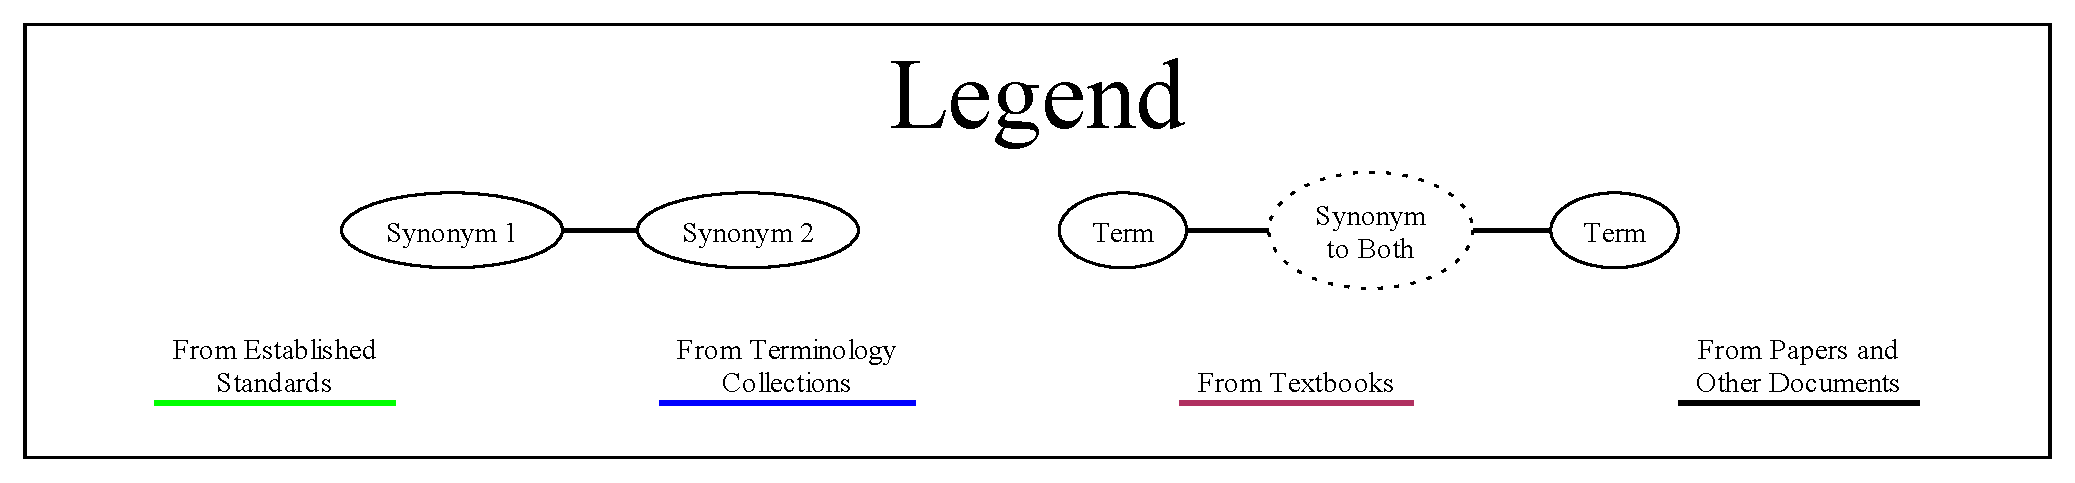
\includegraphics[width=\linewidth]{assets/graphs/manual/expSynLegend.pdf}
        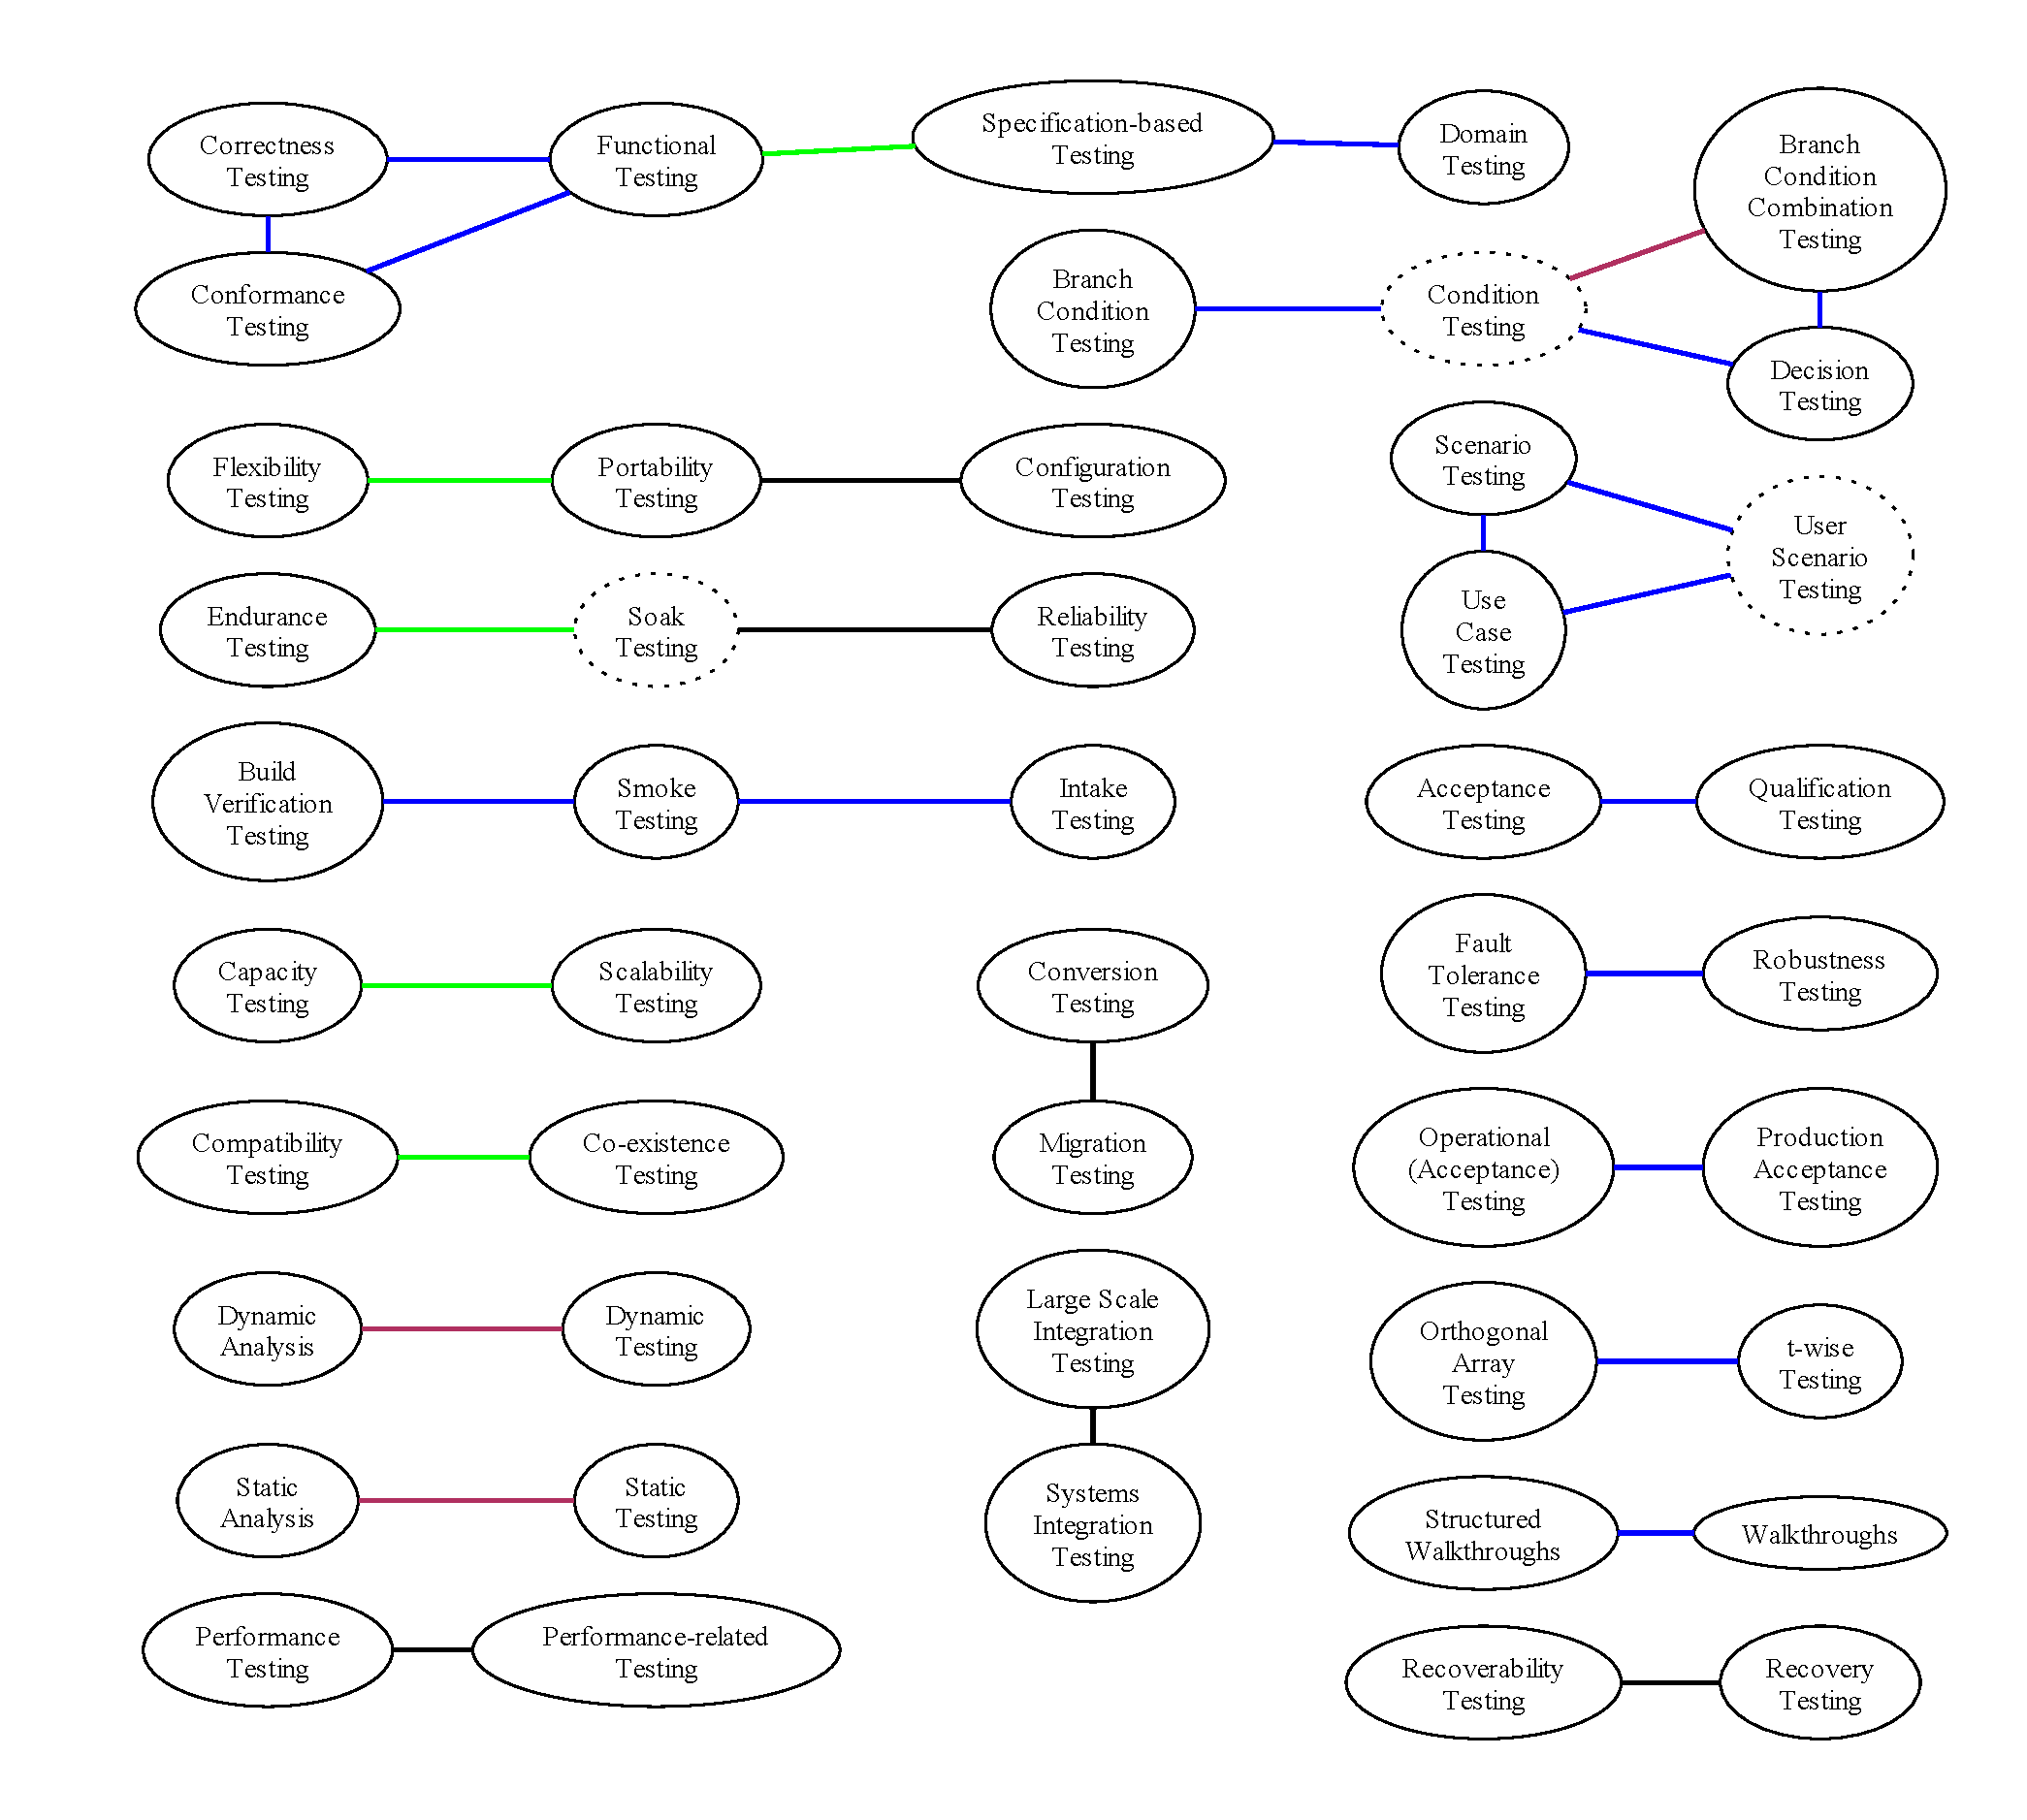
\includegraphics[width=\linewidth]{assets/graphs/manual/expSynGraph.pdf}
        % \vspace{-7mm}
        \caption{Visually meaningful synonym relations
            given explicitly by the literature.}\label{fig:expSynGraph}
    \end{figure}
    \clearpage
    \begin{figure}[bt!]
        \centering
        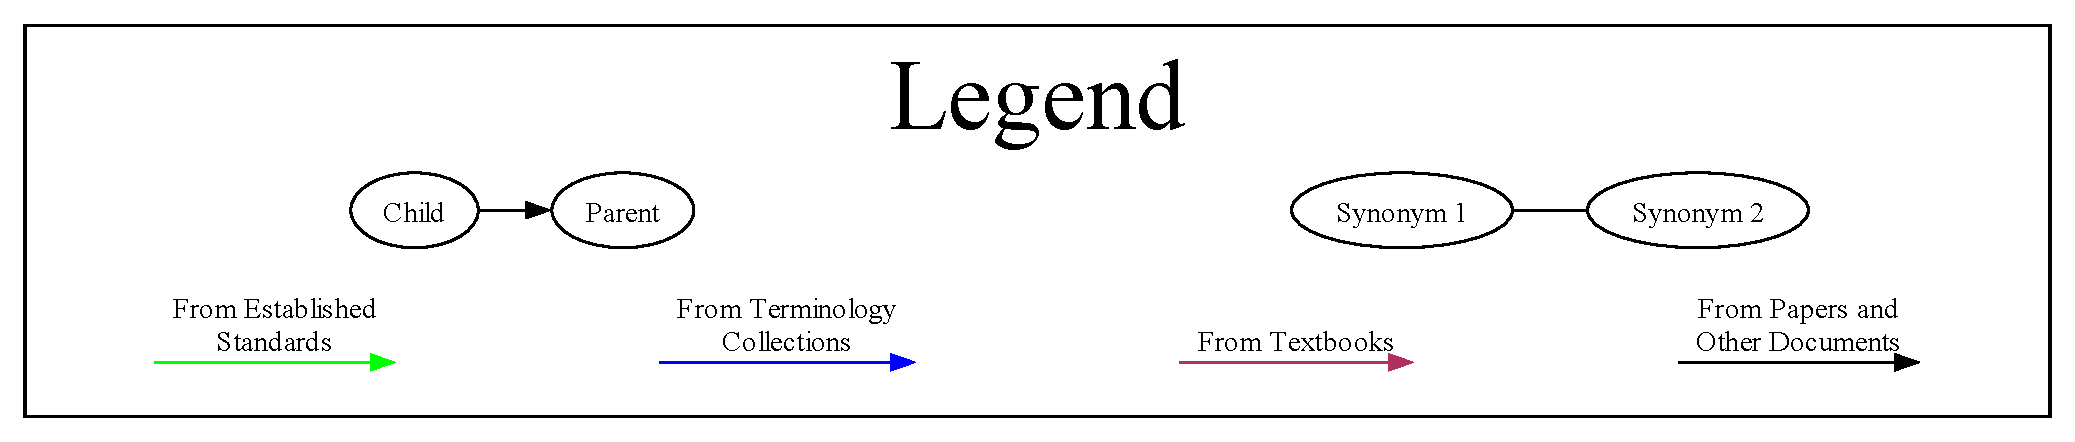
\includegraphics[width=0.48\linewidth]{assets/graphs/manual/expParSynLegend.pdf}
        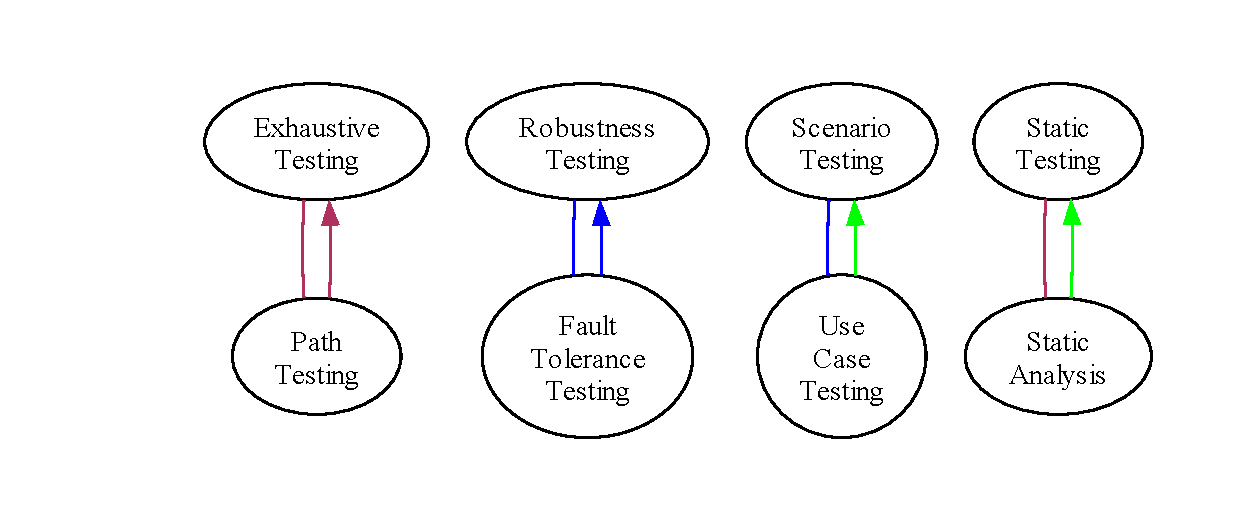
\includegraphics[width=0.5\linewidth]{assets/graphs/manual/expParSynGraph.pdf}
        % \vspace{-7mm}
        \caption{Pairs of test approaches with a parent-child \emph{and} synonym
            relation given explicitly by the literature.}\label{fig:expParSynGraph}
    \end{figure}
\else
\fi

\phantomsection{}\label{parSyns}
\parSynIntro{}\ifnotpaper. We visualize the pairs where both
relations are explicit in \Cref{fig:expParSynGraph} and list all
identified pairs in \Cref{tab:parSyns}, as well as pairs where we infer a
flaw in \Cref{infParSyns} for completeness\else\ and list the most
prominent in \Cref{tab:parSyns}\fi. Of
particular note is the relation between path testing and exhaustive testing.
While \citet[p.~421]{vanVliet2000} claims that path testing done completely
``is equivalent to exhaustively testing the program''\ifnotpaper\footnote{The
        contradictory definitions of path testing given in \flawref{path-test}
        add another layer of complexity to this claim.}\fi, this overlooks the
effects of input data \ifnotpaper
    (\citealp[pp.~129\==130]{IEEE2021c}; \citealp[p.~121]{Patton2006};
    \citealp[p.~467]{PetersAndPedrycz2000})
\else
    \cite[p.~467]{PetersAndPedrycz2000}, \cite[p.~121]{Patton2006},
    \cite[p.~129\==130]{IEEE2021c}
\fi and implementation issues \citetext{p.~476} % \citep[p.~476]{PetersAndPedrycz2000}
on the code's behaviour. Exhaustive testing
requires ``all combinations of input values \emph{and} preconditions \dots{}
[to be] tested'' \ifnotpaper (\citealp[p.~4, emphasis added]{IEEE2022};
    similar in \citealpISTQB{}; \citealp[p.~121]{Patton2006})\else
    \cite[p.~4]{IEEE2022} (similar in \citealpISTQB{},
    \cite[p.~121]{Patton2006})\fi.
% Flaw count (WRONG, SYNS): {vanVliet2000} | {IEEE2022} {IEEE2021c} ISTQB {PetersAndPedrycz2000} {Patton2006}

% % TODO: re-investigate this after going through the rest of ISO/IEC/IEEE 29119
% \ifnotpaper
%     \subsubsection{Definition Flaws}\label{defs}

%     \citet{IEEE2022, IEEE2021a, IEEE2021b, IEEE2021c}, from the
%     ISO/IEC/IEEE 29119 family of standards, mention the following 28 test
%     approaches without defining them. This means that out of the 119 test
%     approaches they mention, more than 20\% have no associated definition!

%     However, the previous version of this standard, \citeyearpar{IEEE2013},
%     generally explained two, provided references for two, and explicitly defined
%     one of these terms, for a total of five definitions that could (should) have
%     been included in \citeyearpar{IEEE2022}! These terms have been
%     \underline{underlined}\ifnotpaper%
%         , \emph{italicized}, and \textbf{bolded}, respectively%
%     \fi. Additionally, entries marked with an asterisk* were defined (at least
%     partially) in \citeyearpar{IEEE2017}, which would have been available when
%     creating this family of standards. These terms bring the total count of
%     terms that could (should) have been defined to eleven; almost 40\% of
%     these undefined test approaches could have been defined!

%     \begin{itemize}
%         \item \underline{Acceptance Testing*}
%         \item Alpha Testing*
%         \item Beta Testing*
%         \item BCP Testing
%         \item Capture-Replay Driven Testing
%         \item Configuration Testing*
%         \item Data-driven Testing
%         \item Error-based Testing
%         \item Factory Acceptance Testing
%         \item Fault Injection Testing
%         \item Functional Suitability Testing (also mentioned but not defined in
%               \citep{IEEE2017}; Functional Suitability*)
%         \item Inspections*
%         \item \underline{Integration Testing}*
%         \item Maintenance Testing
%         \item Model Verification
%         \item Operational Acceptance Testing
%         \item Orthogonal Array Testing
%         \item Peer Reviews
%         \item Production Verification Testing
%         \item Recovery Testing* (Failover/Recovery Testing, Back-up/Recovery
%               Testing, \formatPaper{\textbf}{Backup and Recovery Testing*},
%               Recovery*; see \Cref{recov-flaw})
%         \item Response-Time Testing
%         \item \formatPaper{\emph}{Reviews} (ISO/IEC 20246) (Code Reviews*)
%               (IEEE 1028, the IEEE ``Standard for Software Reviews and Audits'',
%               is cited in the bibliography!)
%         \item Scalability Testing (given as a synonym of ``capacity
%               testing''; see \Cref{scal-flaw})
%         \item Statistical Testing
%         \item System Integration Testing (System Integration*)
%         \item System Testing* (also mentioned but not defined in \citep{IEEE2013})
%         \item \formatPaper{\emph}{Unit Testing*}
%               (IEEE 1008, the IEEE ``Standard for Software Unit Testing'',
%               is cited in the bibliography!)
%         \item User Acceptance Testing
%     \end{itemize}
% \fi

\ifnotpaper
    \subsection{Operational (Acceptance) Testing}\label{oat-flaw}
    \paragraph{\texttt{(CONTRA, LABELS)}}
    % Flaw count (CONTRA, LABELS): {IEEE2022} ISTQB | {SWEBOK2024} {ISO_IEC2018} {IEEE2017} {SWEBOK2014}
    There are two names that the literature gives to this test approach:
    \begin{itemize}
        \item \emph{\acf{operat}} (\citealp[p.~22]{IEEE2022};
              \citealpISTQB{}) and
        \item \emph{\acf{ot}} (\citealp{ISO_IEC2018};
              \citealp[p.~303]{IEEE2017}; \citealp[p.~6\=/9, in the context of
                  software engineering operations]{SWEBOK2024};
              \citealp[pp.~4\=/6, 4\=/9]{SWEBOK2014}).
    \end{itemize}

    \paragraph{\texttt{(CONTRA, SYNS)}}
    % Flaw count (CONTRA, SYNS): {Firesmith2015}
    % Assertion: {LambdaTest2024} {BocchinoAndHamilton1996}
    \refHelper \citet[p.~30]{Firesmith2015} lists the above terms separately,
    but they are considered synonyms elsewhere \citep{LambdaTest2024,
        BocchinoAndHamilton1996}\todo{find more academic sources}; since
    \citeauthor{Firesmith2015} does not define these terms, it is hard to
    evaluate \ifnotpaper his \else its \fi distinction.
\fi

\subsection{Recovery Testing}\label{recov-flaw}

``Recovery testing'' is ``testing \dots\ aimed at verifying
software restart capabilities after a system crash or other disaster''
\citep[p.~5\=/9]{SWEBOK2024} including ``recover[ing] the data directly affected
and re-establish[ing] the desired state of the system'' \ifnotpaper
    (\citealp{ISO_IEC2023a}; similar in \citealp[p.~7\=/10]{SWEBOK2024})
\else \cite{ISO_IEC2023a} (similar in \cite[p.~7\=/10]{SWEBOK2024}) \fi
so that the system ``can perform required functions'' \citep[p.~370]{IEEE2017}.
However, the literature also describes similar test approaches with vague or
non-existent distinctions between them. We describe these approaches and their
flaws here and present the relations between them in \Cref{fig:rec-graph-current}.

\NewDocumentCommand\subDRT{s}{given as a subtype of ``disaster/recovery
    testing'' which tests if ``operation of the test item can
    be transferred to a different operating site''
    \IfBooleanTF{#1}{\citetext{p.~37}}{\citeyearpar[p.~37]{IEEE2021c}},
    even though this is \emph{explicitly} excluded from its definition on the
    same page!}

%% again, maybe convert to \paragraph ?
\begin{itemize}
    \item \emph{Recoverability testing} evaluates ``how well a system or
          software can recover data during an interruption or failure''
          \ifnotpaper (\citealp[p.~7\=/10]{SWEBOK2024}; \else
              \cite[p.~7\=/10]{SWEBOK2024} (\fi similar in \citealp{ISO_IEC2023a})
          and ``re-establish the desired state of the system''
          \citeyearpar{ISO_IEC2023a}. \refHelper \citet[p.~47]{Kam2008}
          gives this as a synonym for ``recovery testing''.
    \item \emph{Disaster/recovery testing} evaluates if a system
          can ``return to normal operation after a hardware
          or software failure'' \citep[p.~140]{IEEE2017} or if ``operation of
          the test item can be transferred to a different operating site and
          \dots\ be transferred back again once the failure has been
          resolved'' \citeyearpar[p.~37]{IEEE2021c}.
          \begin{itemize}
              \item \texttt{(OVER, DEFS)}
                    % Flaw count (OVER, DEFS): {IEEE2017} | {IEEE2021c}
                    These two definitions seem to describe different aspects of
                    the system, where the first is intrinsic to the
                    hardware/software and the second might not be, making this
                    term nonatomic.
          \end{itemize}
    \item \emph{Backup and recovery testing} ``measures the
          degree to which system state can be restored from backup within
          specified parameters of time, cost, completeness, and accuracy in
          the event of failure'' \citep[p.~2]{IEEE2013}. This may be what is
          meant by ``recovery testing'' in the context of performance-related
          testing \citeyearpar[Fig.~2]{IEEE2022}.
    \item \emph{Backup/recovery testing} determines the ability of a system
          ``to restor[e] from back-up memory in the event of failure, without
          transfer[ing] to a different operating site or back-up system''
          \citep[p.~37]{IEEE2021c}.
          \begin{itemize}
              %   \item \texttt{(OVER, DEFS)}
              %         % Flaw count (OVER, DEFS): {IEEE2021c} | {IEEE2017}
              %         This definition corresponds to the first definition of
              %         ``disaster/recovery testing'' given by
              %         \citeyearpar[p.~140]{IEEE2017}.
              \item \texttt{(CONTRA, PARS)}
                    % Flaw count (CONTRA, PARS): {IEEE2021c} | {IEEE2021c}
                    This \subDRT{}
              \item \texttt{(OVER, LABELS)}
                    % Flaw count (OVER, LABELS): {IEEE2021c} | {IEEE2013}
                    Its name is also quite similar to ``backup and
                    recovery testing'', adding further confusion.
          \end{itemize}
    \item \emph{Failover/recovery testing} determines the
          ability ``to mov[e] to a back-up system in the event of failure,
          without transfer[ing] to a different operating site''
          \citep[p.~37]{IEEE2021c}.
          \begin{itemize}
              \item \texttt{(CONTRA, PARS)}
                    % Flaw count (CONTRA, PARS): {IEEE2021c} | {IEEE2021c}
                    This is also \subDRT*{}
              \item \texttt{(AMBI, PARS)}
                    % Flaw count (AMBI, PARS): {IEEE2021c}
                    % Assertion: {SWEBOK2024} ISTQB
                    While not explicitly related to recovery, \emph{failover
                        testing} ``validates the SUT's ability to manage heavy
                    loads or unexpected failure to continue typical operations''
                    \citep[p.~5\=/9]{SWEBOK2024} by entering a ``backup
                    operational mode in which [these responsibilities] \dots\
                    are assumed by a secondary system'' \citepISTQB{}. Its name
                    implies that it is a child of ``failover/recovery testing''
                    but its definition makes it more broad (as it includes handling
                    ``heavy loads'' where failover/recovery testing does not)
                    which may reverse the direction of this relation.
              \item \texttt{(AMBI, SYNS)}
                    % Flaw count (AMBI, SYNS): {IEEE2021c} | implied by {Firesmith2015}
                    \refHelper \citet[p.~56]{Firesmith2015} uses the term
                    ``failover and recovery testing'' which may be a synonym of
                    ``failover/recovery testing''.
          \end{itemize}
    \item \emph{Restart \& recovery (testing)} is listed as a test approach by
          \citet[Fig.~5]{Gerrard2000a} but is not defined \texttt{(MISS, DEFS)}
          % Flaw count (MISS, DEFS): {Gerrard2000a}
          and may simply be a synonym to ``recovery testing'' \texttt{(AMBI, SYNS)}.
          % Flaw count (AMBI, SYNS): {Gerrard2000a}
\end{itemize}

\subsection{Scalability Testing}\label{scal-flaw}

\paragraph{\texttt{(CONTRA, SYNS)}}

% Flaw count (CONTRA, SYNS): {IEEE2021c} | {Firesmith2015} {Bas2024}
\citeauthor{IEEE2021c} \citeyearpar[p.~39]{IEEE2021c} give
``scalability testing'' as a synonym of ``capacity testing''
while other sources differentiate between the two \ifnotpaper
    (\citealp[p.~53]{Firesmith2015}; \citealp[pp.~22\==23]{Bas2024})%
\else \cite[p.~53]{Firesmith2015}, \cite[pp.~22\==23]{Bas2024}\fi.

\paragraph{\texttt{(CONTRA, DEFS)}}

% Flaw count (CONTRA, DEFS): {IEEE2021c} | implied by {ISO_IEC2023a}
\citeauthor{IEEE2021c} \citeyearpar[p.~39]{IEEE2021c} also include the external
modification of the system as part of ``scalability'' but
\citet{ISO_IEC2023a} \multiAuthHelper{describe} it as testing the ``capability
of a product to handle growing or shrinking workloads or to adapt its capacity
to handle variability'', implying that this is done by the system itself.

\paragraph{\texttt{(WRONG, LABELS)}}

% Flaw count (WRONG, LABELS): {SWEBOK2024}
\citeauthor{SWEBOK2024} \citeyearpar[p.~5\=/9]{SWEBOK2024} says ``scalability
testing evaluates the capability to use and learn the system and the user
documentation'' and ``focuses on the system's effectiveness in supporting user
tasks and the ability to recover from user errors''. \swebokScalDef{}.

% \subsection{Performance Testing}
% \label{perf-test-ambiguity}

% Similarly, ``performance'' and ``performance efficiency'' are both given as
% software qualities by \ifnotpaper\citeauthor{IEEE2017}\else
%       \cite[p.~319]{IEEE2017}\fi, with the latter defined as the ``performance
% relative to the amount of resources used under stated conditions''
% \ifnotpaper\citeyearpar[p.~319]{IEEE2017} \fi or the ``capability of a product
% to perform its functions within specified time and throughput parameters and be
% efficient in the use of resources under specified conditions'' \citep{ISO_IEC2023a}.
% Initially, there didn't seem to be any meaningful distinction between the two,
% although the term ``performance testing'' is defined
% \ifnotpaper\citeyearpar[p.~320]{IEEE2017}\else\citetext{p.~320}\fi\
% and used by \ifnotpaper\citeauthor{IEEE2017}\else\cite{IEEE2017}\fi\ and the term
% ``performance efficiency testing'' is \emph{also} used by
% \ifnotpaper\citeauthor{IEEE2017}\else\cite{IEEE2017}\fi\ (but not defined
% explicitly). \ifnotpaper Further discussion\thesisissueref{43} brought us to
%       the conclusion \else It can then be concluded \fi that ``performance
% efficiency testing'' is a subset of ``performance testing'', and the
% difference of ``relative to the amount of resources used'' or ``be efficient in
% the use of resources'' between the two is meaningful.

\subsection{Compatibility Testing}\label{compat-flaw}

\paragraph{\texttt{(OVER, DEFS)}}
% Flaw count (OVER, DEFS): {IEEE2022} | {IEEE2017} ISTQB {ISO_IEC2023a}
``Compatibility testing'' is defined as ``testing that measures the
degree to which a test item can function satisfactorily alongside
other independent products in a shared environment (co-existence),
and where necessary, exchanges information with other systems or
components (interoperability)'' \citep[p.~3]{IEEE2022}. This
definition is nonatomic as it combines the ideas of ``co-existence''
and ``interoperability''.

\paragraph{\texttt{(WRONG, SYNS)}}
% Flaw count (WRONG, SYNS): implied by {IEEE2021c} | {IEEE2022}
The ``interoperability'' element of ``compatibility testing'' is explicitly
excluded by \citet[p.~37]{IEEE2021c}, (incorrectly) implying that ``compatibility
testing'' and ``co-existence testing'' are synonyms.

\paragraph{\texttt{(AMBI, SYNS)}}
% Flaw count (AMBI, SYNS): {Kam2008} | {IEEE2022}
Furthermore, the definition of ``compatibility testing'' in
\citet[p.~43]{Kam2008} unhelpfully says ``see \emph{interoperability testing}'',
adding another layer of confusion to the direction of their relationship.

\paragraph{\texttt{(WRONG, LABELS)}}
% Flaw count (WRONG, LABELS): {IEEE2022}
% Assertion: {ISO_IEC2023a} {IEEE2022} {IEEE2021c} {IEEE2017} ISTQB
\refHelper \citet[pp.~22, 43]{IEEE2022} \multiAuthHelper{say}
``interoperability testing helps confirm that applications can work on multiple
operating systems and devices'', but this seems to instead describe
``portability testing'', which evaluates the ``capability of a product to be
adapted to changes in its requirements, contexts of use, or system environment''
\ifnotpaper
    (\citealp{ISO_IEC2023a}; similar in \citealp[p.~7]{IEEE2022};
    \citeyear[pp.~184, 329]{IEEE2017}; \citealpISTQB{})\else
    \cite{ISO_IEC2023a} (similar in \citeyear[pp.~184, 329]{IEEE2017},
    \citealp[p.~7]{IEEE2022}, \cite{ISTQB})\fi, such as being ``transferred
from one hardware \dots{} environment to another'' \citep[p.~39]{IEEE2021c}.

\section{Recommendations}\label{recs}

As we have shown in \Cref{flaws}, ``testing is a mess'' \citetext{Mosser,
    2023, priv.\ comm.}! It will take a lot of time, effort, expertise, and
training to organize these terms (and their relations) logically. However, the
hardest step is often the first one, so we attempt to give some examples of how
this ``rationalization'' can occur. These changes often arise when we notice an
issue with the current state of the terminology and think about what \emph{we}
would do to make it better. We do not claim that these are correct, unbiased,
or exclusive, just that they can be used as an inspiration for those wanting to
pick up where we leave off.

When redefining terms, we seek to make them:
\begin{enumerate}
    \item Atomic (e.g., disaster/recovery testing seems to have two
          disjoint definitions)
    \item Straightforward (e.g., backup and recovery testing's definition
          implies the idea of performance, but its name does not
          \ifnotpaper; failover/recovery testing, failover and recovery
          testing, and failover testing are all given separately\fi)
    \item Consistent (e.g., backup/recovery testing and failover/recovery
          testing explicitly exclude an aspect included in its parent
          disaster/recovery testing)
\end{enumerate}
Likewise, we seek to eliminate classes of flaws that can be detected
automatically, such as test approaches that are given as synonyms to multiple
distinct approaches (\Cref{multiSyns}) or as parents of themselves
(\Cref{selfPars}), or pairs of approaches with both a parent-child \emph{and}
synonym relation (\Cref{parSyns}).\todo{Same label to different phantomsections;
    is that OK?}

We give recommendations for the areas of \ifnotpaper operational (acceptance)
    testing (\Cref{oat-test-rec}), \fi recovery testing (\Cref{rec-test-rec}),
scalability testing (\Cref{scal-test-rec}), performance-related testing
(\Cref{perf-test-rec}), and compatibility testing (\Cref{compat-test-rec}). We
provide graphical representations (see \Cref{\ifnotpaper app-rel-vis\else tools\fi})
of these subsets when helpful in \recFigs{}, in which arrows representing
relations between approaches are coloured based on the source tier (see
\Cref{source-tiers}) that defines them. We colour all proposed approaches and
relations orange. \ifnotpaper We also include inferred approaches and relations
    in grey for completeness, although they are not explicitly given in the
    literature (see \Cref{infers}).

    \subsection{Operational (Acceptance) Testing}\label{oat-test-rec}
    Since this terminology is not standardized (see \Cref{oat-flaw}), we
    propose that ``\acf{operat}'' and ``\acf{ot}'' are treated as
    synonyms for a type of acceptance testing (\citealp[p.~22]{IEEE2022};
    \citealpISTQB{}) that focuses on ``non-functional'' attributes of the system
    \citep{LambdaTest2024}\todo{find more academic sources}. Indeed, this is how we
    track this approach in \ourApproachGlossary{}! We define it as ``test[ing] to
    determine the correct installation, configuration and operation of a module and
    that it operates securely in the operational environment'' \citep{ISO_IEC2018}
    or to ``evaluate a system or component in its operational environment''
    \citep[p.~303]{IEEE2017}, particularly ``to determine if operations and/or
    systems administration staff can accept [it]'' \citepISTQB{}.
\fi

\subsection{Recovery Testing}\label{rec-test-rec}
% The following terms should be used in place of the current terminology to
% more clearly distinguish between different recovery-related test approaches.
% The result of the proposed terminology, along with their relations, is
% demonstrated in \Cref{fig:rec-graph-proposed}.

To remedy the flaws we describe in \Cref{recov-flaw}, we recommend that the
literature uses these terms more consistently, resulting in the improved graph
in \Cref{fig:rec-graph-proposed}. The following proposals ``recapture''
information from the literature more consistently:

\begin{enumerate}
    \item Prefer the term ``recoverability testing'' over ``recovery testing''
          to indicate its focus on a system's \emph{ability} to recover, not its
          \emph{performance} of recovering \citep[p.~47]{Kam2008}. ``Recovery
          testing'' may be an acceptable synonym, since it seems to be more
          prevelant in the literature.
    \item Introduce the term \emph{recovery performance testing} when evaluating
          performance metrics of a system's recovery as a subapproach of
          recoverability testing and performance-related testing\footnote{
              See \Cref{perf-test-rec}.}
          (\citealp[Fig.~2]{IEEE2022}; \citeyear[p.~2]{IEEE2013}).
    \item Introduce separate terms for the different methods of recovery which
          are all subapproaches of recoverability testing:
          \begin{enumerate}
              \item from backup memory (\emph{backup recovery testing})
                    (\citealp[p.~37]{IEEE2021b}; \citeyear[p.~2]{IEEE2013}),
              \item from a back-up system (\emph{failover testing})
                    (\citealp[p.~5\=/9]{SWEBOK2024}; \citealpISTQB{}), or
              \item by transferring operations elsewhere (\emph{transfer
                        recovery testing}) \citep[p.~37]{IEEE2021b}.
          \end{enumerate}
\end{enumerate}

\recoveryGraphs{}

% \begin{itemize}
%     \item \textbf{Recoverability Testing:} ``Testing \dots\ aimed at
%           verifying software restart capabilities after a system crash or
%           other disaster'' \citep[p.~5-9]{SWEBOK2024} including ``recover[ing]
%           the data directly affected and re-establish[ing] the desired state
%           of the system''
%           \ifnotpaper
%               (\citealp{ISO_IEC2023a}; similar in \citealp[p.~7-10]{SWEBOK2024})
%           \else
%               \cite{ISO_IEC2023a} (similar in \cite[p.~7-10]{SWEBOK2024})
%           \fi so that the system ``can perform
%           required functions'' \citep[p.~370]{IEEE2017}. ``Recovery testing''
%           will be a synonym, as in \citep[p.~47]{Kam2008}, since it is the
%           more prevalent term throughout various sources, although
%           ``recoverability testing'' is preferred to indicate that this
%           explicitly focuses on the \emph{ability} to
%           recover, not the \emph{performance} of recovering.
%     \item \textbf{Failover Testing:} Testing that ``validates the SUT's
%           ability to manage heavy loads or unexpected failure to continue
%           typical operations'' \cite[p.~5-9]{SWEBOK2024} by entering a
%           ``backup operational mode in which [these responsibilities] \dots\
%           are assumed by a secondary system'' \citepISTQB{}. This will
%           replace ``failover/recovery testing'', since it is more clear, and
%           since this is one way that a system can recover from failure, it
%           will be a subset of ``recovery testing''.
%     \item \textbf{Transfer Recovery Testing:} Testing to evaluate if,
%           in the case of a failure, ``operation of the test item can be
%           transferred to a different operating site and \dots\ be transferred
%           back again once the failure has been resolved''
%           \citeyearpar[p.~37]{IEEE2021b}. This replaces the second definition
%           of ``disaster/recovery testing'', since the first is just a
%           description of ``recovery testing'', and could potentially be
%           considered as a kind of failover testing. This may not be
%           intrinsic to the hardware/software (e.g., may be the responsibility
%           of humans/processes).
%     \item \textbf{Backup Recovery Testing:} Testing that determines the
%           ability ``to restor[e] from back-up memory in the event of failure''
%           \citep[p.~37]{IEEE2021b}. The qualification that this occurs
%           ``without transfer[ing] to a different operating site or back-up
%           system'' \citetext{p.~37} \emph{could} be made explicit, but this is
%           implied since it is separate from transfer recovery testing and
%           failover testing, respectively.
%     \item \textbf{Recovery Performance Testing:} Testing ``how well a system or
%           software can recover \dots\ [from] an interruption or failure''
%           \ifnotpaper
%               (\citealp[p.~7-10]{SWEBOK2024}; similar in \citealp{ISO_IEC2023a})
%           \else
%               \cite[p.~7-10]{SWEBOK2024} (similar in \cite{ISO_IEC2023a})
%           \fi ``within specified parameters of time, cost, completeness, and
%           accuracy'' \citep[p.~2]{IEEE2013}. The distinction between the
%           performance-related elements of recovery testing seemed to be
%           meaningful\thesisissueref{40}, but was not captured consistently
%           by the literature. This will be a subset of ``performance-related
%           testing'' \ifnotpaper (see \Cref{perf-test-rec}) \fi
%           as ``recovery testing'' is in \citep[p.~22]{IEEE2022}. This could
%           also be extended into testing the performance of specific elements
%           of recovery (e.g., failover performance testing), but this be too
%           fine-grained and may better be captured as an
%           \hyperref[orth-test]{orthogonally derived test approach}.
% \end{itemize}

\subsection{Scalability Testing}\label{scal-test-rec}

We describe the issues with scalability testing terminology in \Cref{scal-flaw}
and show the relations between related approaches (as described by the
literature) in \Cref{fig:scal-graph-current}. These flaws are resolved and/or
explained by other sources! Taking this extra information into account results
in \Cref{fig:scal-graph-proposed} and provides a more accurate description of
scalability testing.

\paragraph{\texttt{(CONTRA, SYNS)}}
\citeauthor{IEEE2021b} \citeyearpar[p.~39]{IEEE2021b} define ``scalability
testing'' as the testing of a system's ability to ``perform under conditions
that may need to be supported in the future''.
%, which ``may include assessing what level of additional resources (e.g.
% memory, disk capacity, network bandwidth) will be required to support
% anticipated future loads''.
This focus on ``the future''
is supported by \citetISTQB{}, \ifnotpaper who define \else which defines \fi
``scalability'' as ``the degree to which a component or system can be adjusted
for changing capacity''\ifnotpaper; the original source they reference agrees,
defining it as ``the measure of a system's ability to be upgraded to
accommodate increased loads'' \citep[p.~381]{GerrardAndThompson2002}\fi. In
contrast, capacity testing focuses on the system's present state, evaluating
the ``capability of a product to meet requirements for the maximum limits of a
product parameter''
%, such as the number of concurrent users, transaction
% throughput, or database size 
\citep{ISO_IEC2023a}. Therefore, it these terms should \emph{not} be synonyms,
as done by \ifnotpaper
    \citet[p.~53]{Firesmith2015} and \citet[pp.~22\==23]{Bas2024}\else
    \cite[p.~53]{Firesmith2015} and \cite[pp.~22\==23]{Bas2024}\fi.

\paragraph{\texttt{(CONTRA, DEFS)}}

There seems to be an underlying reason that sources disagree on whether
external modification of the system is part of scalability testing.
\citeauthor{SWEBOK2024} \citeyearpar[p.~5\=/9]{SWEBOK2024} claim that one
objective of elasticity testing is ``to evaluate scalability'', implying that
\citep{ISO_IEC2023a}'s notion of ``scalability'' actually refers to
``elasticity''! This makes sense in the context of other definitions
provided by \citet{SWEBOK2024}:
\begin{itemize}
    \item \textbf{Scalability:} ``the software's ability to increase and
          scale up on its nonfunctional requirements, such as load, number of
          transactions, and volume of data'' \citetext{p.~5\=/5}. Based on this
          definition, scalability testing is then a subtype of load testing
          and volume testing, as well as potentially transaction flow testing.
    \item \textbf{Elasticity Testing\ifnotpaper\footnote{This definition seems
                      correct but its source is unclear; see
                      \flawref{elas-ref}.}\fi:} testing that ``assesses
          the ability of the \acs{sut} \dots\ to rapidly expand or shrink
          compute, memory, and storage resources without compromising the
          capacity to meet peak utilization'' \citetext{p.~5\=/9}. Based on this
          definition, elasticity testing is then a subtype of memory
          management testing (with both being a subtype of resource
          utilization testing) and stress testing.
\end{itemize}
This distinction is consistent with how the terms are used in industry:
\citet{Pandey2023}\thesisissueref{35} says that scalability is the ability to
``increase \dots\ performance or efficiency as demand increases over time'',
while elasticity allows a system to ``tackle changes in the workload [that]
occur for a short period''.

\paragraph{\texttt{(WRONG, LABELS)}}

\citeauthor{SWEBOK2024} \citeyearpar[p.~5\=/9]{SWEBOK2024}'s definition of
``scalability testing'' is completely separate from the definitions of
``scalability'', ``capacity'', and ``elasticity'' discussed above! Therefore,
this definition and its related synonym relations should simply be disregarded
since they are inconsistent with the rest of the literature.

\scalGraphs{}

\subsection{Performance(-related) Testing}
\label{perf-test-rec}

``Performance testing'' is defined as testing ``conducted to evaluate the
degree to which a test item accomplishes its designated functions''
\ifnotpaper
    (\citealp[p.~7]{IEEE2022}; \citeyear[p.~320]{IEEE2017}; similar in
    \citeyear[pp.~38-39]{IEEE2021b}; \citealp[p.~1187]{Moghadam2019})%
\else
    \cite[p.~320]{IEEE2017}, \cite[p.~7]{IEEE2022} (similar in
    \cite[pp.~38-39]{IEEE2021b}, \cite[p.~1187]{Moghadam2019})%
\fi. It does this
by ``measuring the performance metrics''
\ifnotpaper
    (\citealp[p.~1187]{Moghadam2019}; similar in \citealpISTQB{})
\else
    \cite[p.~1187]{Moghadam2019} (similar in \cite{ISTQB})
\fi (such as the ``system's capacity for growth''
\citep[p.~23]{Gerrard2000b}), ``detecting the functional problems appearing
under certain execution conditions'' \citep[p.~1187]{Moghadam2019}, and
``detecting violations of non-functional requirements under expected and
stress conditions'' \ifnotpaper
    (\citealp[p.~1187]{Moghadam2019}; similar in \citealp[p.~5-9]{SWEBOK2024})%
\else
    \cite[p.~1187]{Moghadam2019} (similar in \cite[p.~5-9]{SWEBOK2024})%
\fi. It is performed either \dots\
\begin{enumerate}
    \item ``within given constraints of time and other resources''
          \ifnotpaper
              (\citealp[p.~7]{IEEE2022}; \citeyear[p.~320]{IEEE2017};
              similar in \citealp[p.~1187]{Moghadam2019})%
          \else
              \cite[p.~320]{IEEE2017}, \cite[p.~7]{IEEE2022} (similar
              in \cite[p.~1187]{Moghadam2019})%
          \fi, or
    \item ``under a `typical' load'' \citep[p.~39]{IEEE2021b}.
\end{enumerate}

It is listed as a subset of performance-related testing, which is defined as
testing ``to determine whether a test item performs as required when it is
placed under various types and sizes of `load'\,'' \citeyearpar[p.~38]{IEEE2021b},
along with other approaches like load and capacity testing
\citep[p.~22]{IEEE2022}. Note that ``performance, load and stress testing might
considerably overlap in many areas'' \citep[p.~1187]{Moghadam2019}.
In contrast, \citet[p.~5-9]{SWEBOK2024}
gives ``capacity and response time'' as examples of ``performance
characteristics'' that performance testing would seek to ``assess'', which
seems to imply that these are subapproaches to performance testing instead.
This is consistent with how some sources treat ``performance testing'' and
``performance-related testing'' as synonyms \ifnotpaper
    (\citealp[p.~5-9]{SWEBOK2024}; \citealp[p.~1187]{Moghadam2019})%
\else \cite[p.~5-9]{SWEBOK2024}, \cite[p.~1187]{Moghadam2019}%
\fi, as noted in \Cref{syns}. This makes sense because of how general the
concept of ``performance'' is; most definitions of ``performance testing'' seem
to treat it as a category of tests.

However, it seems more consistent to infer
that the definition of ``performance-related testing'' is the more general one
often assigned to ``performance testing'' performed ``within given constraints
of time and other resources'' \ifnotpaper (\citealp[p.~7]{IEEE2022};
    \citeyear[p.~320]{IEEE2017}; similar in \citealp[p.~1187]{Moghadam2019})%
\else \cite[p.~320]{IEEE2017}, \cite[p.~7]{IEEE2022}
    (similar in \cite[p.~1187]{Moghadam2019})\fi, and
``performance testing'' is a subapproach of this performed ``under a `typical'
load'' \citep[p.~39]{IEEE2021b}. This has other implications for relations
between these types of testing; for example, ``load testing'' usually occurs
``between anticipated conditions of low, typical, and peak usage''
\ifnotpaper (\citealp[p.~5]{IEEE2022}; \citeyear[p.~39]{IEEE2021b};
    \citeyear[p.~253]{IEEE2017}\todo{OG IEEE 2013}; \citealpISTQB{})%
\else \cite[p.~253]{IEEE2017}, \cite{ISTQB}, \cite[p.~5]{IEEE2022},
    \cite[p.~39]{IEEE2021b}\fi, so it is a child of ``performance-related
testing'' and a parent of ``performance testing''.

After these changes, some finishing touches remain. The ``self-loops''
mentioned in \Cref{selfPars} provide no new information and can be removed.
Similarly, the term ``soak testing'' can be removed. Since it is given as a
synonym to both ``endurance testing'' \emph{and} ``reliability testing'' (see
\Cref{multiSyns}), it makes sense to just use these terms instead of one that
is potentially ambiguous. These changes (along with those from
\Cref{rec-test-rec,scal-test-rec} made implicitly) result in
the relations shown in \Cref{fig:perf-graph}.

\begin{paperFigure}
    \centering
    \performanceGraph{}
    \caption{Proposed relations between rationalized ``performance-related testing'' terms.}
    \label{fig:perf-graph}
\end{paperFigure}

\subsection{Compatibility Testing}\label{compat-test-rec}
``Co-existence'' and ``interoperability'' are often defined separately
\ifnotpaper (\citealp[pp.~73, 237]{IEEE2017}; \citealpISTQB{})%
\else \cite[pp.~73, 237]{IEEE2017}, \cite{ISTQB}\fi, sometimes explicitly as a
decomposition of ``compatibility'' \citep{ISO_IEC2023a}! Following this
precedent, ``co-existence testing'' and ``interoperability testing'' should be
defined as their own test approaches to make their definitions atomic;
\citet{IEEE2017} \multiAuthHelper{define} ``interoperability testing''
\citetext{p.~238} but not ``co-existence testing''. The term ``compatibility
testing'' may still be a useful test approach to define, but it should be
defined independently of its children: ``co-existence testing'' and
``interoperability testing''.


\section{Conclusion}

While a good starting point, the current literature on software testing has
much room to grow. The many flaws create unnecessary barriers to
software testing. While there is merit to allowing the state-of-the-practice
terminology to descriptively guide how terminology is used, there
may be a need to prescriptively structure terminology to intentionally
differentiate between and organize various test approaches. Future work in this
area will continue to investigate the current use of terminology, in
particular \nameref{undef-terms}, determine if IEEE's current
\nameref{cats-def} are sufficient, and rationalize the definitions of
and relations between terms.

\section*{Acknowledgment}
\label{acknowledgements}

ChatGPT was used to help generate supplementary Python code for constructing
graphs and generating \LaTeX{} code, including regex. ChatGPT and GitHub
Copilot were both used for assistance with \LaTeX{} formatting. ChatGPT and
ProWritingAid were both used for proofreading.
\ifblind{ChatGPT also provided some of the approaches in \Cref{stop-crit}.
[Additional acknowledgement suppressed.]}{Jason Balaci's
\href{https://github.com/balacij/McMaster-Thesis-Template}
{McMaster thesis template} provided many helper \LaTeX{} functions.
A special ``thank you'' to Christopher William Schankula for help with
\LaTeX{}, Reed Mullanix with formal logic, and various friends for
discussing software testing with me and providing many of the approaches in
\Cref{stop-crit} (we also used ChatGPT for the latter). Finally, \supersAck{}.}

\newpage

\bibliographystyle{IEEEtran}
\bibliography{IEEEabrv,references}

\end{document}
